\documentclass[a4paper,12pt]{article}   % papír A4, písmo 12 bodu
\usepackage[utf8x]{inputenc}            %kodovaní UTF-8
\usepackage{ucs}                        %kodovani unicode
\usepackage[czech]{babel}               %podpora cestiny
\usepackage[T1]{fontenc}                %pouzij variantu pisma T1 (hacky, carky)
\usepackage[left=2cm,right=1.5cm,top=2cm,bottom=2cm]{geometry} %okraje stranky
\usepackage{amsmath,amsfonts,amssymb}   %podpora matematiky
\usepackage{gensymb,marvosym}           %symboly celsius (\celsius) apod.
%\usepackage{mathptmx}                   %font Times New Roman s~podporou matematiky
%\usepackage{times}                      %font Times New Roman (matematika pismem Computer Modern) 
\usepackage{parskip}                    %mezera mezi odstavci
%\usepackage[document]{ragged2e}         %text zarovany vlevo
\usepackage[none]{hyphenat} \sloppy     %slova nedelit a~nepretekat
\usepackage{titlesec}
\setcounter{secnumdepth}{4}
\clubpenalty 10000                      %kontrolovat sirotky
\widowpenalty 10000                     %kontrolovat vdovy
%\usepackage{setspace} \onehalfspacing   %podpora pro zmenu radkovani + radkovani 1,5
\usepackage{enumerate}                  %podpora pro zmenu cislovani
\usepackage{fancyhdr}                   %vlastni zahlavi a~zapati
\usepackage{graphicx}                   %podpora grafiky
\graphicspath{{materialy/}}                   %vychozi adresar s~obrazky
\usepackage{caption}                    %popisky
\usepackage{subcaption}                 %podpopisky
\usepackage{siunitx}
%\usepackage{MnSymbol,wasysym}
\usepackage[shortlabels]{enumitem}
\usepackage{amsmath}
\usepackage[makeroom]{cancel}
\usepackage{lastpage}                   %zjištění poslední stránky \pageref{LastPage}
\usepackage{url}
\usepackage[unicode]{hyperref}          %klikaci odkazy v~textu
\usepackage{mhchem}
\usepackage{multirow}
%\usepackage{pgfplots}{compat=1.17}
\usepackage{halloweenmath}
\usepackage{datetime}
%vysoké zavorky abs hodnoty
\usepackage{mathtools}
\usepackage{wrapfig}
\DeclarePairedDelimiter\abs{\lvert}{\rvert}
\DeclarePairedDelimiter\norm{\lVert}{\rVert}




\titleclass{\subsubsubsection}{straight}[\subsection]
\newcounter{subsubsubsection}[subsubsection]
\renewcommand\thesubsubsubsection{\thesubsubsection.\arabic{subsubsubsection}}
\renewcommand\theparagraph{\thesubsubsubsection.\arabic{paragraph}} % optional useful if paragraphs are to be numbered


%------------------------ čtvrtá a~pátá úroveň nadpisu ---------------------------
\titleformat{\subsubsubsection}
  {\normalfont\normalsize\bfseries}{\thesubsubsubsection}{1em}{}
\titlespacing*{\subsubsubsection}
{0pt}{3.25ex plus 1ex minus .2ex}{1.5ex plus .2ex}

\makeatletter

\renewcommand\paragraph{\@startsection{paragraph}{5}{\z@}%
  {3.25ex \@plus1ex \@minus.2ex}%
  {-1em}%
  {\normalfont\normalsize\bfseries}}
\renewcommand\subparagraph{\@startsection{subparagraph}{6}{\parindent}%
  {3.25ex \@plus1ex \@minus .2ex}%
  {-1em}%
  {\normalfont\normalsize\bfseries}}
\def\toclevel@subsubsubsection{4}
\def\toclevel@paragraph{5}
\def\toclevel@paragraph{6}
\def\l@subsubsubsection{\@dottedtocline{4}{7em}{4em}}
\def\l@paragraph{\@dottedtocline{5}{10em}{5em}}
\def\l@subparagraph{\@dottedtocline{6}{14em}{6em}}
\makeatother

\setcounter{secnumdepth}{4}
\setcounter{tocdepth}{4}



\makeatletter
\newcommand{\pushright}[1]{\ifmeasuring@#1\else\omit\hfill$\displaystyle#1$\fi\ignorespaces}
\newcommand{\pushleft}[1]{\ifmeasuring@#1\else\omit$\displaystyle#1$\hfill\fi\ignorespaces}
\makeatother

\setlist[enumerate]{itemsep=0mm}
%_____________________________|___________________________|_____________________________%
%                             |                           |                             %
%-----------------------------| ZDE VYPLNIT UDAJE O~PRACI |-----------------------------%
%_____________________________|___________________________|_____________________________%
%                             

\newcommand{\nazev}{tEOretické otázky}                                                        %
\newcommand{\jmeno}{J.D.}                                                     %
\newcommand{\datum}{\today}                                                              %
%---------------------------------------------------------------------------------------%


%-----------------------------| POUŽITÁ MAKRA |-----------------------------%

%\newcommand{\zkratka}{ve výsledku se mi napíše tenhle text}
%\newcommand{}{}
%\newcommand{}{}
%\newcommand{}{}
\newcommand{\tsub}[1]{$_\textrm{#1}$}
\newcommand{\texp}[1]{$^\textrm{#1}$}
\newcommand{\tmu}{$\mu$}
\newcommand{\tpm}{$\pm$}

%zmena velikosti nadpisů
\titleformat*{\section}{\large\bfseries}
\titleformat*{\subsection}{\normalsize\bfseries}
\titleformat*{\subsubsection}{\normalsize\bfseries}



%_______________________________________________________________________________________%
%_______________________________________________________________________________________%


%----------------------------------- KONEC PREAMBULE -----------------------------------%










%-------------------------------------- DOKUMENT --------------------------------------%
%______________________________________________________________________________________%
%definice grafů a~schémat
\usepackage{float}
\newfloat{graf}{hbtp}{ext}
\floatname{graf}{Graf}

\newfloat{schema}{hbtp}{ext}
\floatname{schema}{Schéma}








\begin{document} %%%%%%%%%%%%%%%%%%%%%%%%%%%%%%%%%%%%%%%%%%%%%%%%%%%%%%%%%%%%%%%%%%%%%%%


%Jak číst následující řádky?
%Ve své podstatě se nabízí dvě možnosti a~to podle vaší momentální situace. Buď máte pár dní do zkoušky a~v tom případě bych velice doporučil přečíst text celý. Nemálo tím zvýšíte šance pochopení mnoha problematik. Další možnost je, že máte zkoušku zítra ráno. V~tom případě vás odkazuji na poslední kapitolu, kde je udělán velice fofrový výtah a~jsou sepsány no bullshit odpovědi jdoucí přímo k~věci.


\pagestyle{fancy}                                       %vlastni zahlavi/zapati
\renewcommand{\headrulewidth}{0.5pt}                      %bez linky v~zahlavi
\renewcommand{\footrulewidth}{0pt}                    %linka v~zapati - optional
\lhead{}       \chead{verze \today,~\currenttime} \rhead{}                        %pole zahlavi (prazdna)
\lfoot{} \cfoot{} \rfoot{}   %pole zapati
\begin{wrapfigure}{r}{0.5\textwidth}
    \centering
    
\includegraphics[width=0.1\textwidth]{git-qr.pdf}
\end{wrapfigure}

\begin{center}
    {\Large \textbf{Teoretické otázky ke zkoušce z~předmětu EO1}}\\
    {\normalfont Nejnovější verzi najdete vždy na \url{https://github.com/cviop/EO1-teorie/blob/main/EO1_teoreticke_otazky.pdf}}\\
\end{center}

\textit{Pozn: u kapitol jsou prokliky na skripta. Některé prohlížeče ale bohužel neotevřou PDFko na správném místě} :(
%~\vfill
%\textbf{Jak číst následující řádky?}\\
%Ve své podstatě se nabízí dvě možnosti a~to podle vaší momentální situace. Buď máte pár dní do zkoušky a~v tom případě bych velice doporučil přečíst text celý. Nemálo tím zvýšíte šance pochopení mnoha problematik. Další možnost je, že máte zkoušku zítra ráno. V~tom případě vás odkazuji na poslední kapitolu, kde je udělán velice fofrový výtah a~jsou sepsány no bullshit odpovědi jdoucí přímo k~věci.

%\hfill Hodně štěstí

%\hfill J.D.

%\newpage
\tableofcontents
\newpage

\setcounter{page}{1}
\pagestyle{fancy}                                       %vlastni zahlavi/zapati
\renewcommand{\headrulewidth}{0.5pt}                      %bez linky v~zahlavi
\renewcommand{\footrulewidth}{0pt}                    %linka v~zapati - optional
\lhead{\nazev}       \chead{verze \today} \rhead{\url{github.com/cviop/EO1-teorie}}                        %pole zahlavi (prazdna)
\lfoot{} \cfoot{\thepage} \rfoot{}   %pole zapati

\section{Napište jaké jsou možnosti určení časové odezvy lineárního systému na obecný vstupní signál a~uveďte postup výpočtu. Jaké znáte standardizované odezvy a~k čemu je lze použít}
\subsection*{Odezva na jednotkový skok - přechodová charakteristika}
\href[pdfnewwindow=true]{http://hippo.feld.cvut.cz/vyuka/soubory/ElektronickeObvody.pdf#subsection.7.3.1}{\textit{Odkaz na odpovídající kapitolu v Hospodkových skriptách}}
\begin{figure}[h!]
    \centering
    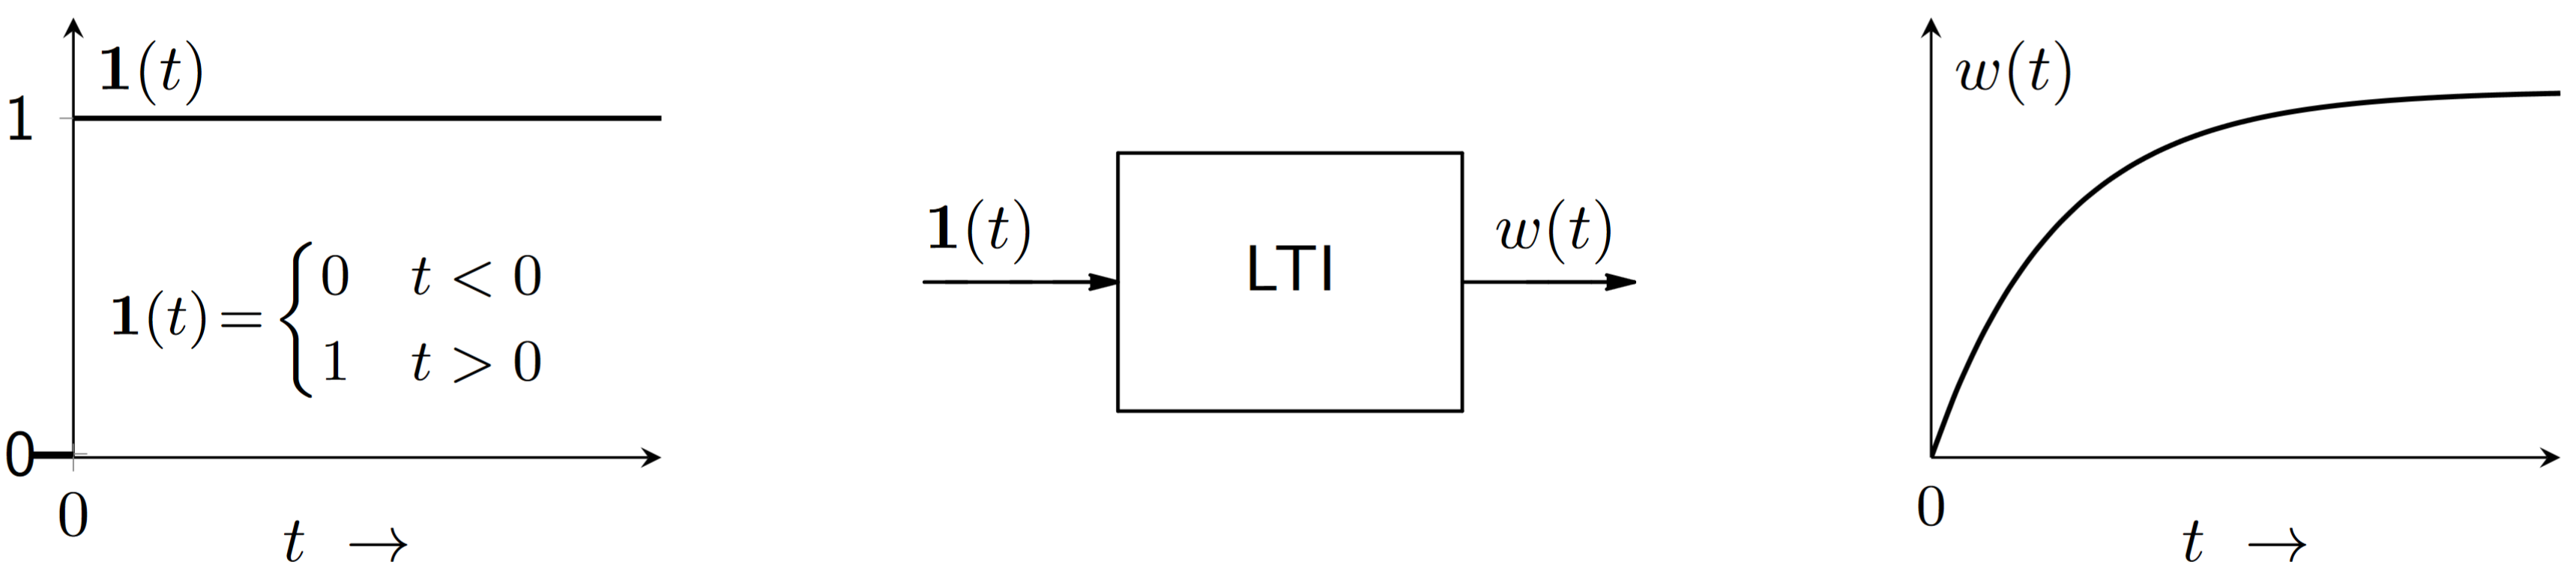
\includegraphics[width=.9\textwidth]{prechodova_odezva.PNG}
    \caption{Přechodová  odezva LTI systému (integrační RC článek)}
\end{figure}
\begin{equation}
    \omega (t) = u_c(t) = 1-e^{-t/RC}
\end{equation}

\subsection*{Odezva na diracův pulz - impulzní charakteristika}
\begin{figure}[h!]
    \centering
    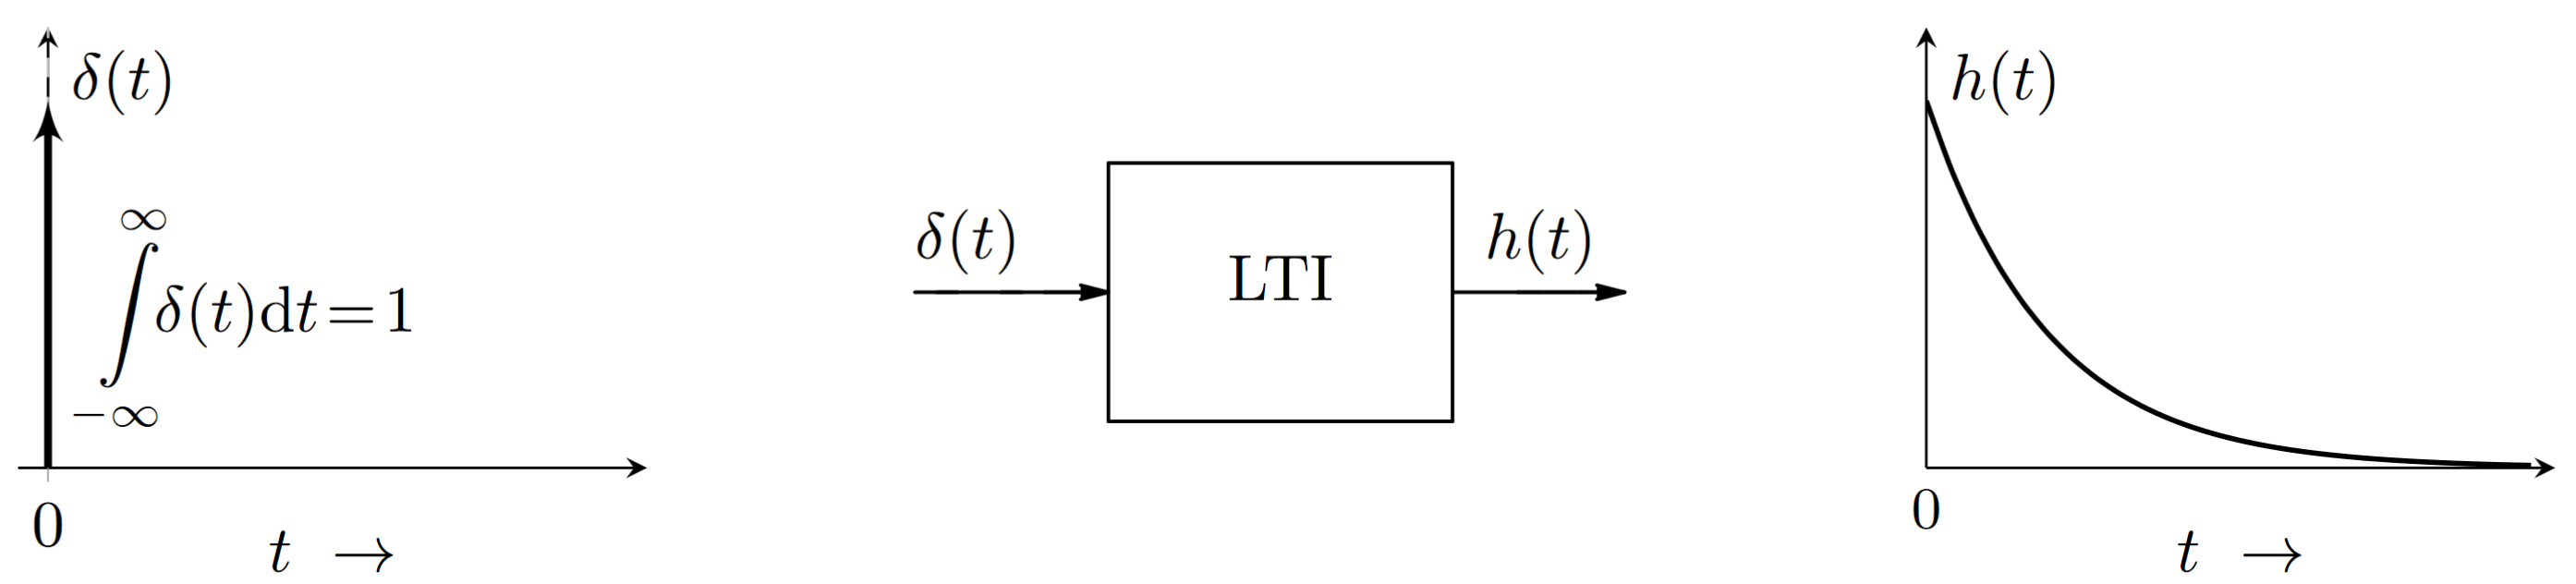
\includegraphics[width=.9\textwidth]{impusni_odezva.PNG}
    \caption{Impulzní charakteristika LTI systému}
\end{figure}
\begin{equation}
    h(t) = \frac{\text{d}\omega(t)}{\text{d}t},~~\omega(t) = \int_0^t h(\tau)\text{d}\tau
\end{equation}






%2
\section{Definujte přenosovou funkci lineárního systému a~napište jaké vlastnosti musí takový systém splňovat. Uveďte co lze pomocí přenosové funkce charakterizovat a~k čemu ji lze využít}
\href[pdfnewwindow=true]{http://hippo.feld.cvut.cz/vyuka/soubory/ElektronickeObvody.pdf#subsection.7.3.2}{\textit{Odkaz na odpovídající kapitolu v Hospodkových skriptách}}

Přenosová funkce (přenos) je definována jako \textbf{podíl} Laplaceových obrazů výstupní a~vstupní veličiny systému při nulových počátečních podmínkách.

\textbf{Linearita}: pokud se zvětší vstupní signál, tak se lineárně zvětší i~signál výstupní.\\
\textbf{Princip superpozice}: součet odezev na dílčí složky signálu je odezva na celkový signál\\
\textbf{Čaová invariance}: je jedno, kdy do signálu pustíme signál

Z přenosové funkce jde zjistit
\begin{itemize}
    \item Stabilita systému
    \item Koeficienty modulové charakteristky
\end{itemize}






%3
\section{Uveďe, co musí splňovat přenosová funkce stabilního systému a~proč demonstrujte na příkladu}
\href[pdfnewwindow=true]{http://hippo.feld.cvut.cz/vyuka/soubory/systemy.pdf#page.15}{\textit{Odkaz na odpovídající kapitolu v Hospodkových skriptách}}

Kořeny \textbf{jmenovatele} přenosové funkce stabilního systému musí ležet v~\textbf{levé komplexní polorovině}, tj. kořeny musí být:
\begin{itemize}
    \item reálné záporné
    \item komplexně sdružené se zápornou reálnou částí
\end{itemize}
Pak je časová odezva pro $t\rightarrow\infty$ konečná, přičemž v~případě komplexních kořenů (pólů) je odezva kmitavá.









%4
\section{Napište přenosovou funkci kmitočtového filtru 2.řádu typu dolní/horní/pásmová propust, případně pásmová zádrž, definujte jednotlivé parametry a~vysvětlete co určují (v kmitočtové a~časové oblasti}
\href[pdfnewwindow=true]{http://hippo.feld.cvut.cz/vyuka/soubory/filtry_prenosy.pdf#page.18}{\textit{Odkaz na odpovídající kapitolu v Hospodkových skriptách}}

\begin{figure}[h!]
    \centering
    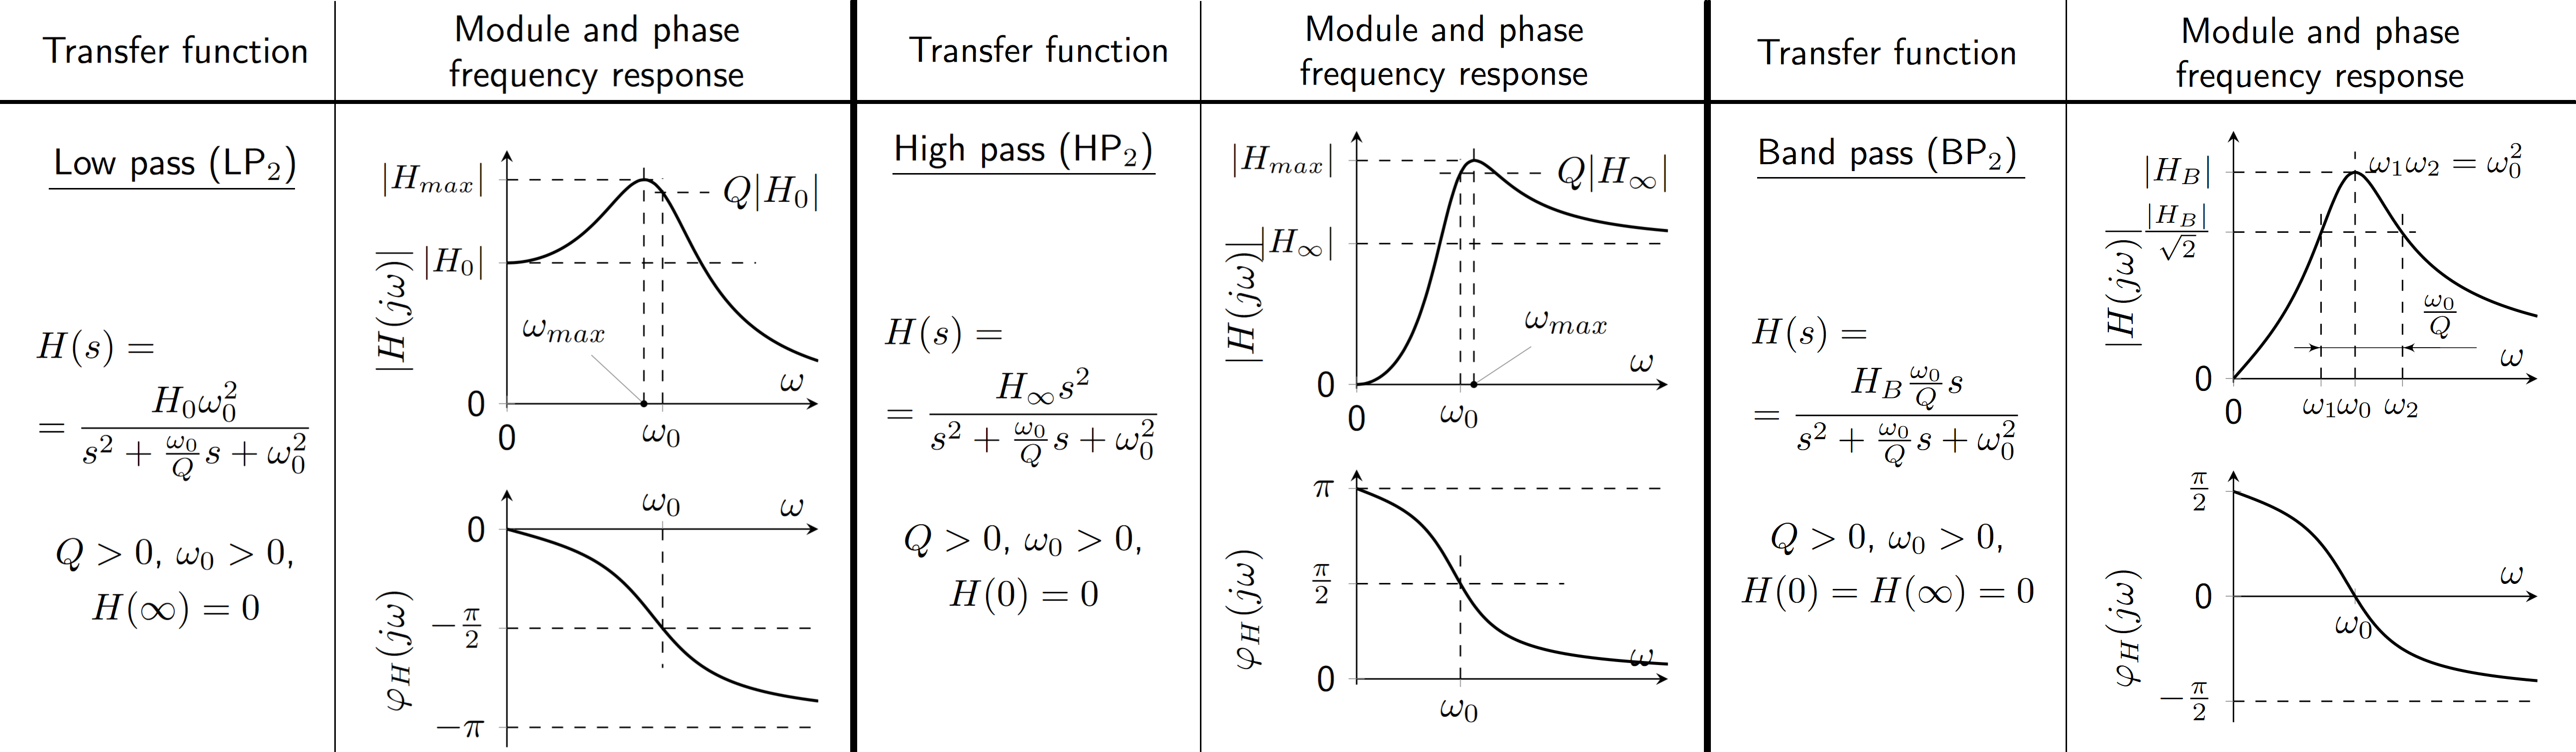
\includegraphics[width=\textwidth]{filtry_2_rad.png}
    \caption[Caption for LOF]{Filtry 2. řádu a~jejich matematický popis\footnotemark}
\end{figure}
\footnotetext{Ideálně vypálit do očí, ale pokud jste odvážní, můžete si všechno odvodit.}

\begin{table}[h!]
    \begin{tabular}{l}
        $s_{p_{1,2}}$ - komplexně sdružený pól\\
        $\omega_0$ - resonanční frekvence\\
        $Q$ - činitel jakosti\\
        $\xi = \frac{1}{2Q}$ - tlumící faktor
    \end{tabular}
\end{table}










%5http://hippo.feld.cvut.cz/vyuka/soubory/filtry_synteza.pdf#page.23
\section{Nakreslete toleranční schéma filtru typu DP/HP/PP/PZ, popište význam charakteristických hodnot. Do schématu pak zakreslete typické modulové charakteristiky pro Besselovu / Butterworthovu / Chebyševovu / inverzní Chebyševovu / Cauerovu aproximaci stejného řádu. Porovnejte jejich vlastnosti v~kmitočtové a~časové oblasti}
\href[pdfnewwindow=true]{http://hippo.feld.cvut.cz/vyuka/soubory/filtry_synteza.pdf#page.23}{\textit{Odkaz na odpovídající kapitolu v Hospodkových skriptách}}

\begin{figure}[H]
    \centering
    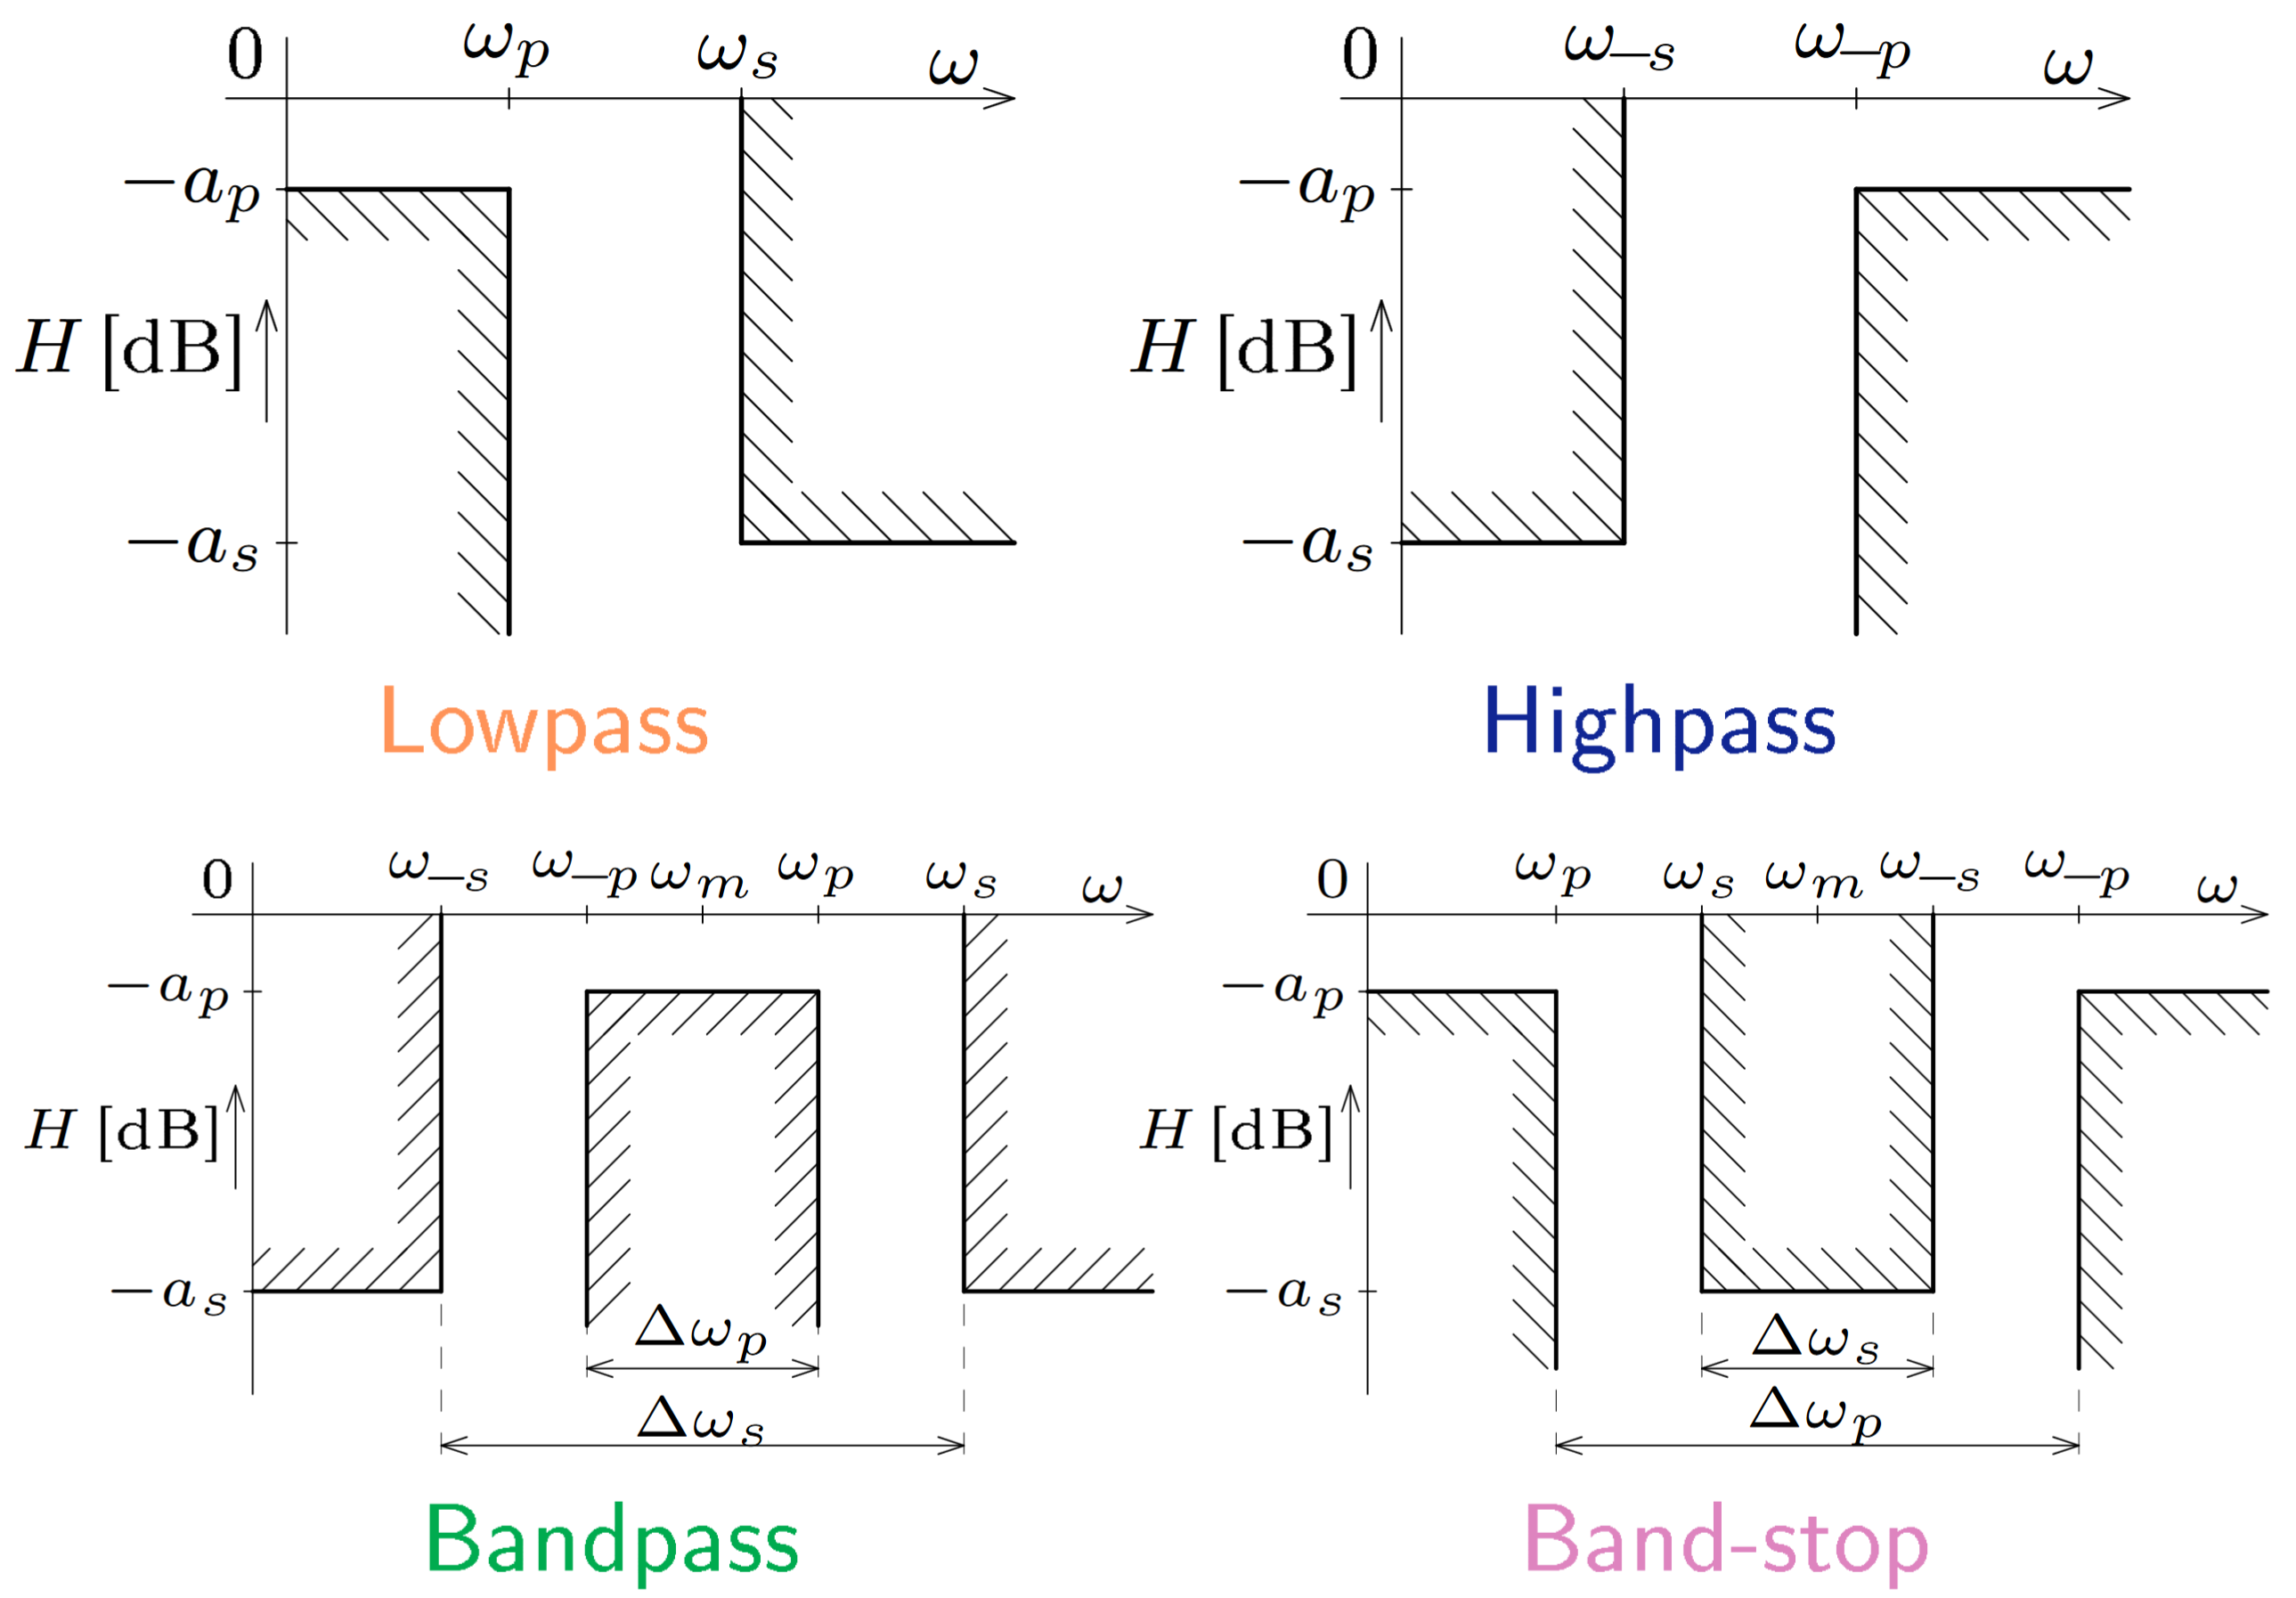
\includegraphics[width=.6\textwidth]{tolerancni_schema.PNG}
    \caption{Toletranční schémata filtrů}
    \label{fig:tolerancni:schemata}
\end{figure}
\begin{graf}[H]
    \centering
    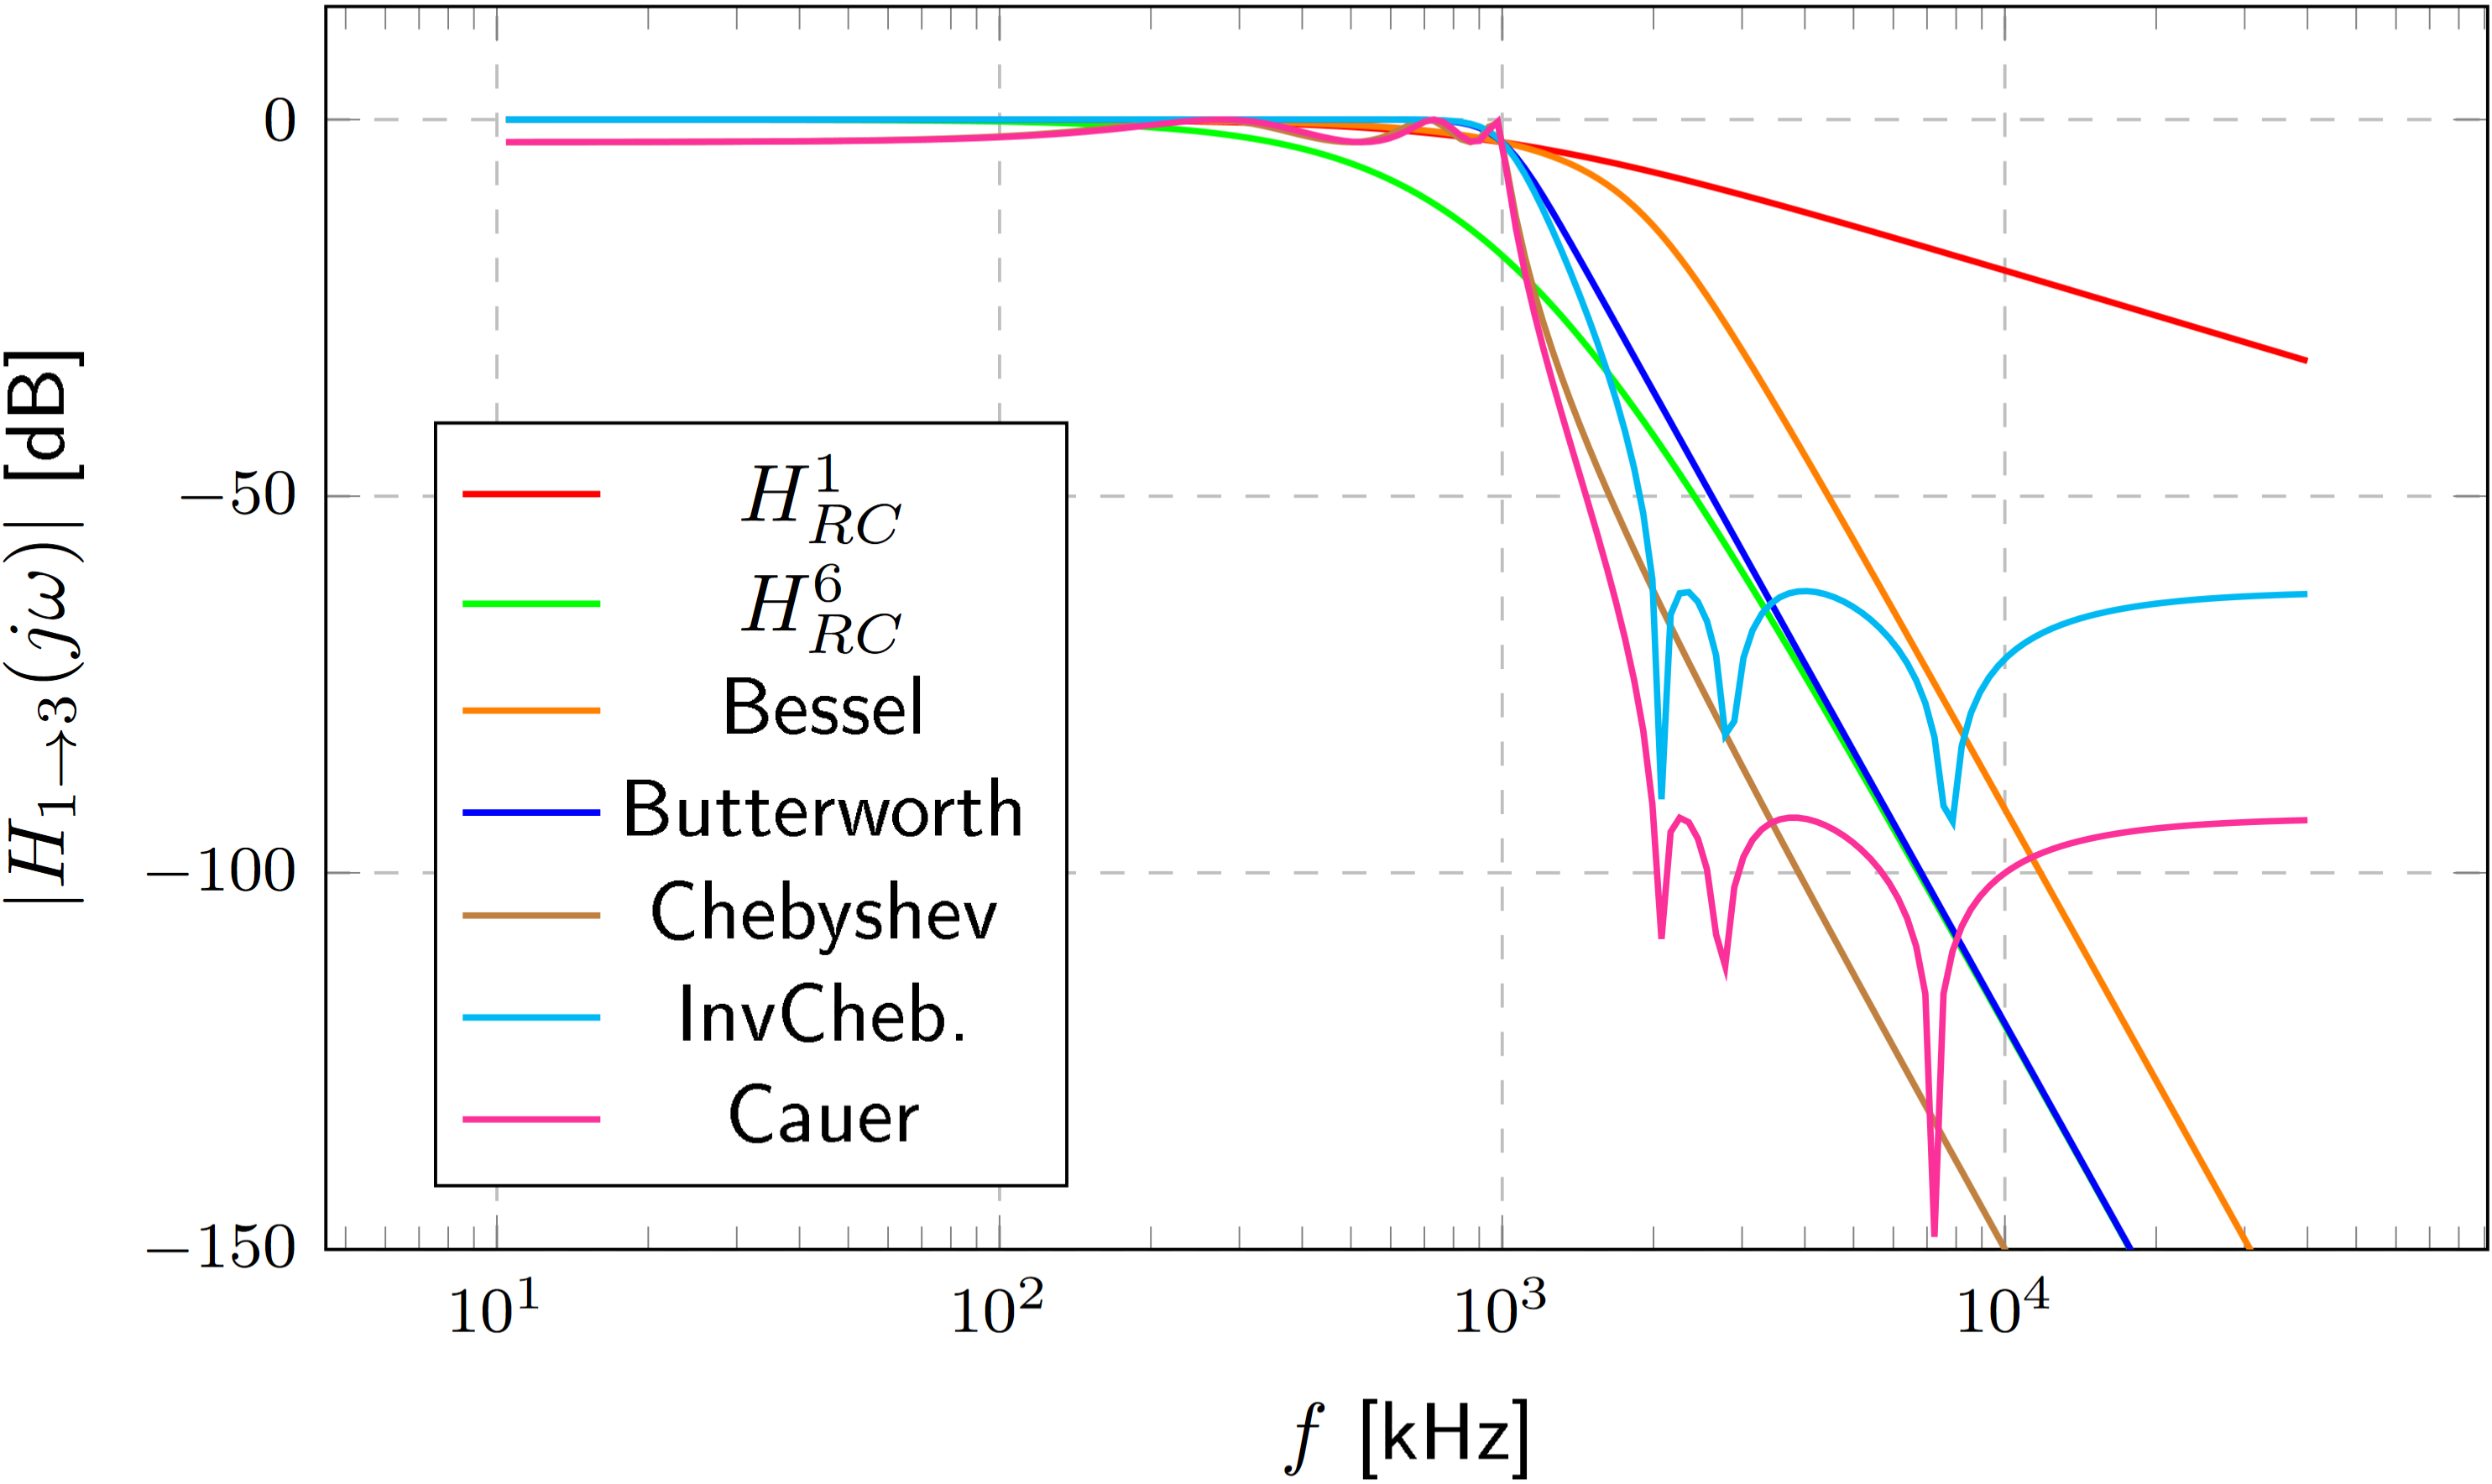
\includegraphics[width=.8\textwidth]{modul-porovnani.PNG}
    \caption{Porovnání modulových charakteristik všech aproximací}
    \label{graf:modul:porovnani}
\end{graf}
\begin{figure}[H]
    \centering
    \begin{subfigure}{.49\textwidth}
        \centering
        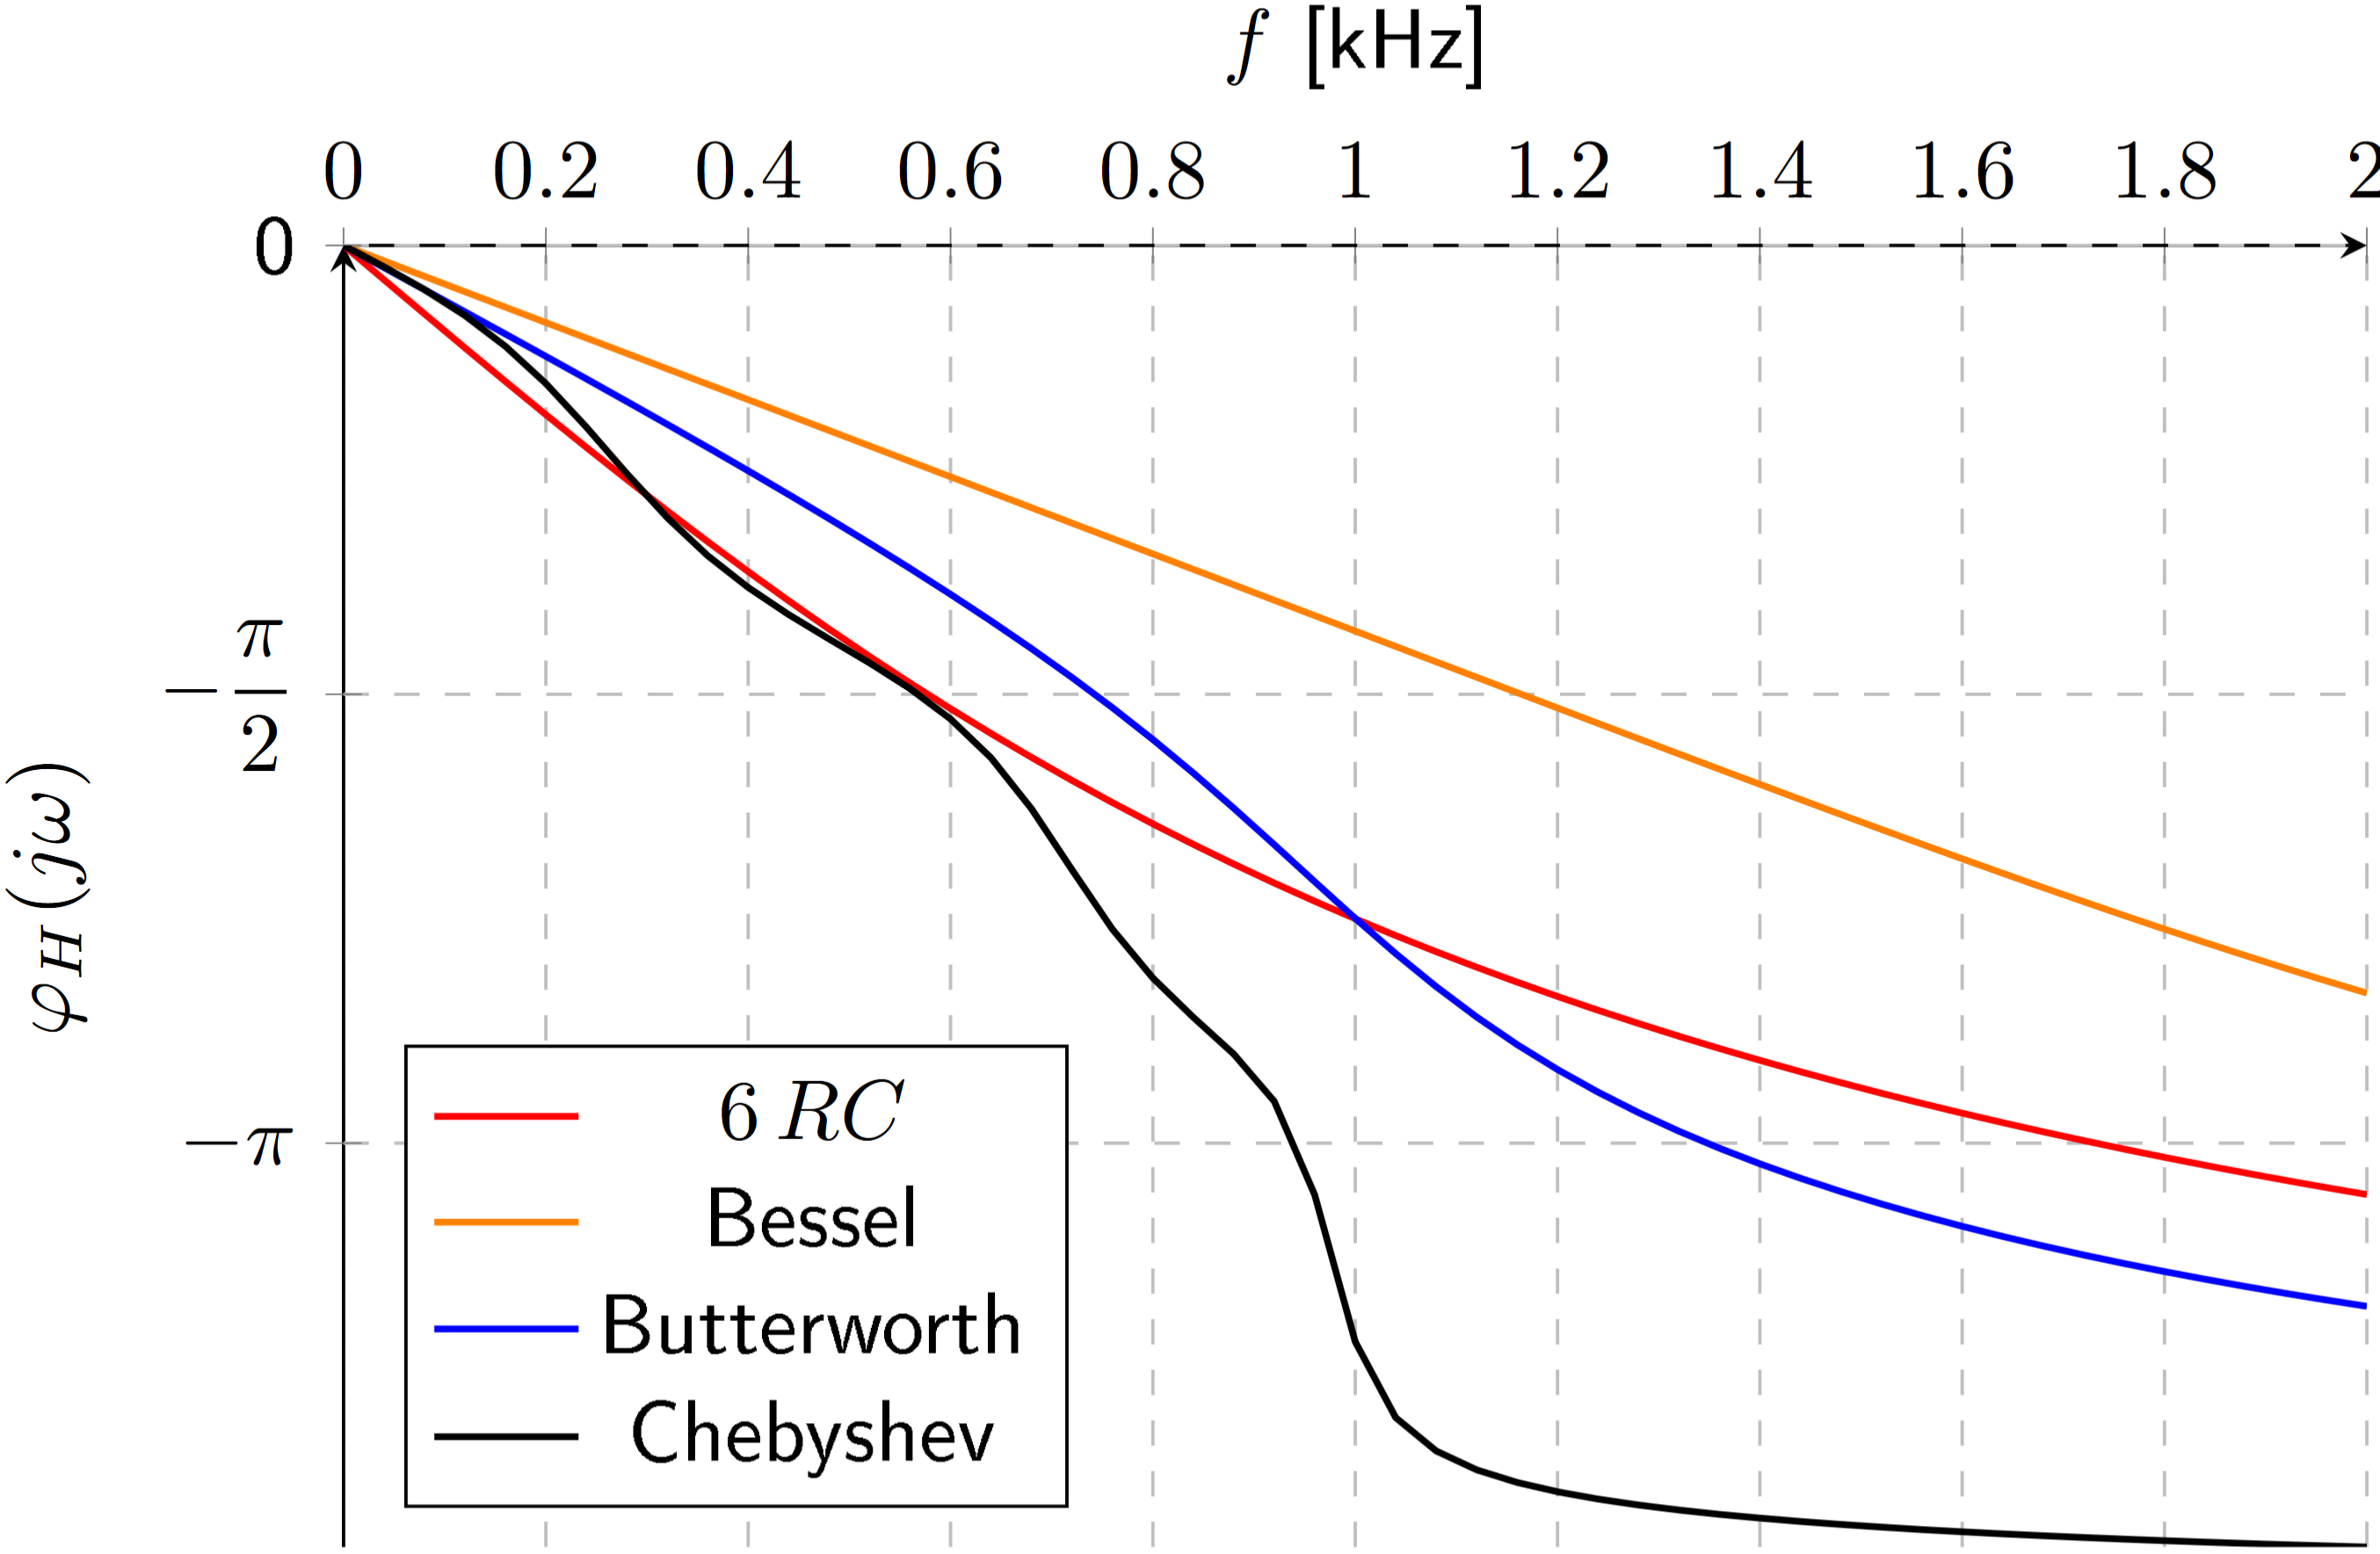
\includegraphics[width=\textwidth]{faze-porovnani.PNG}
        \caption{Porovnání fázových charakteristik}
        \label{graf:faze:porovnani}
    \end{subfigure}
    \begin{subfigure}{.49\textwidth}
        \centering
        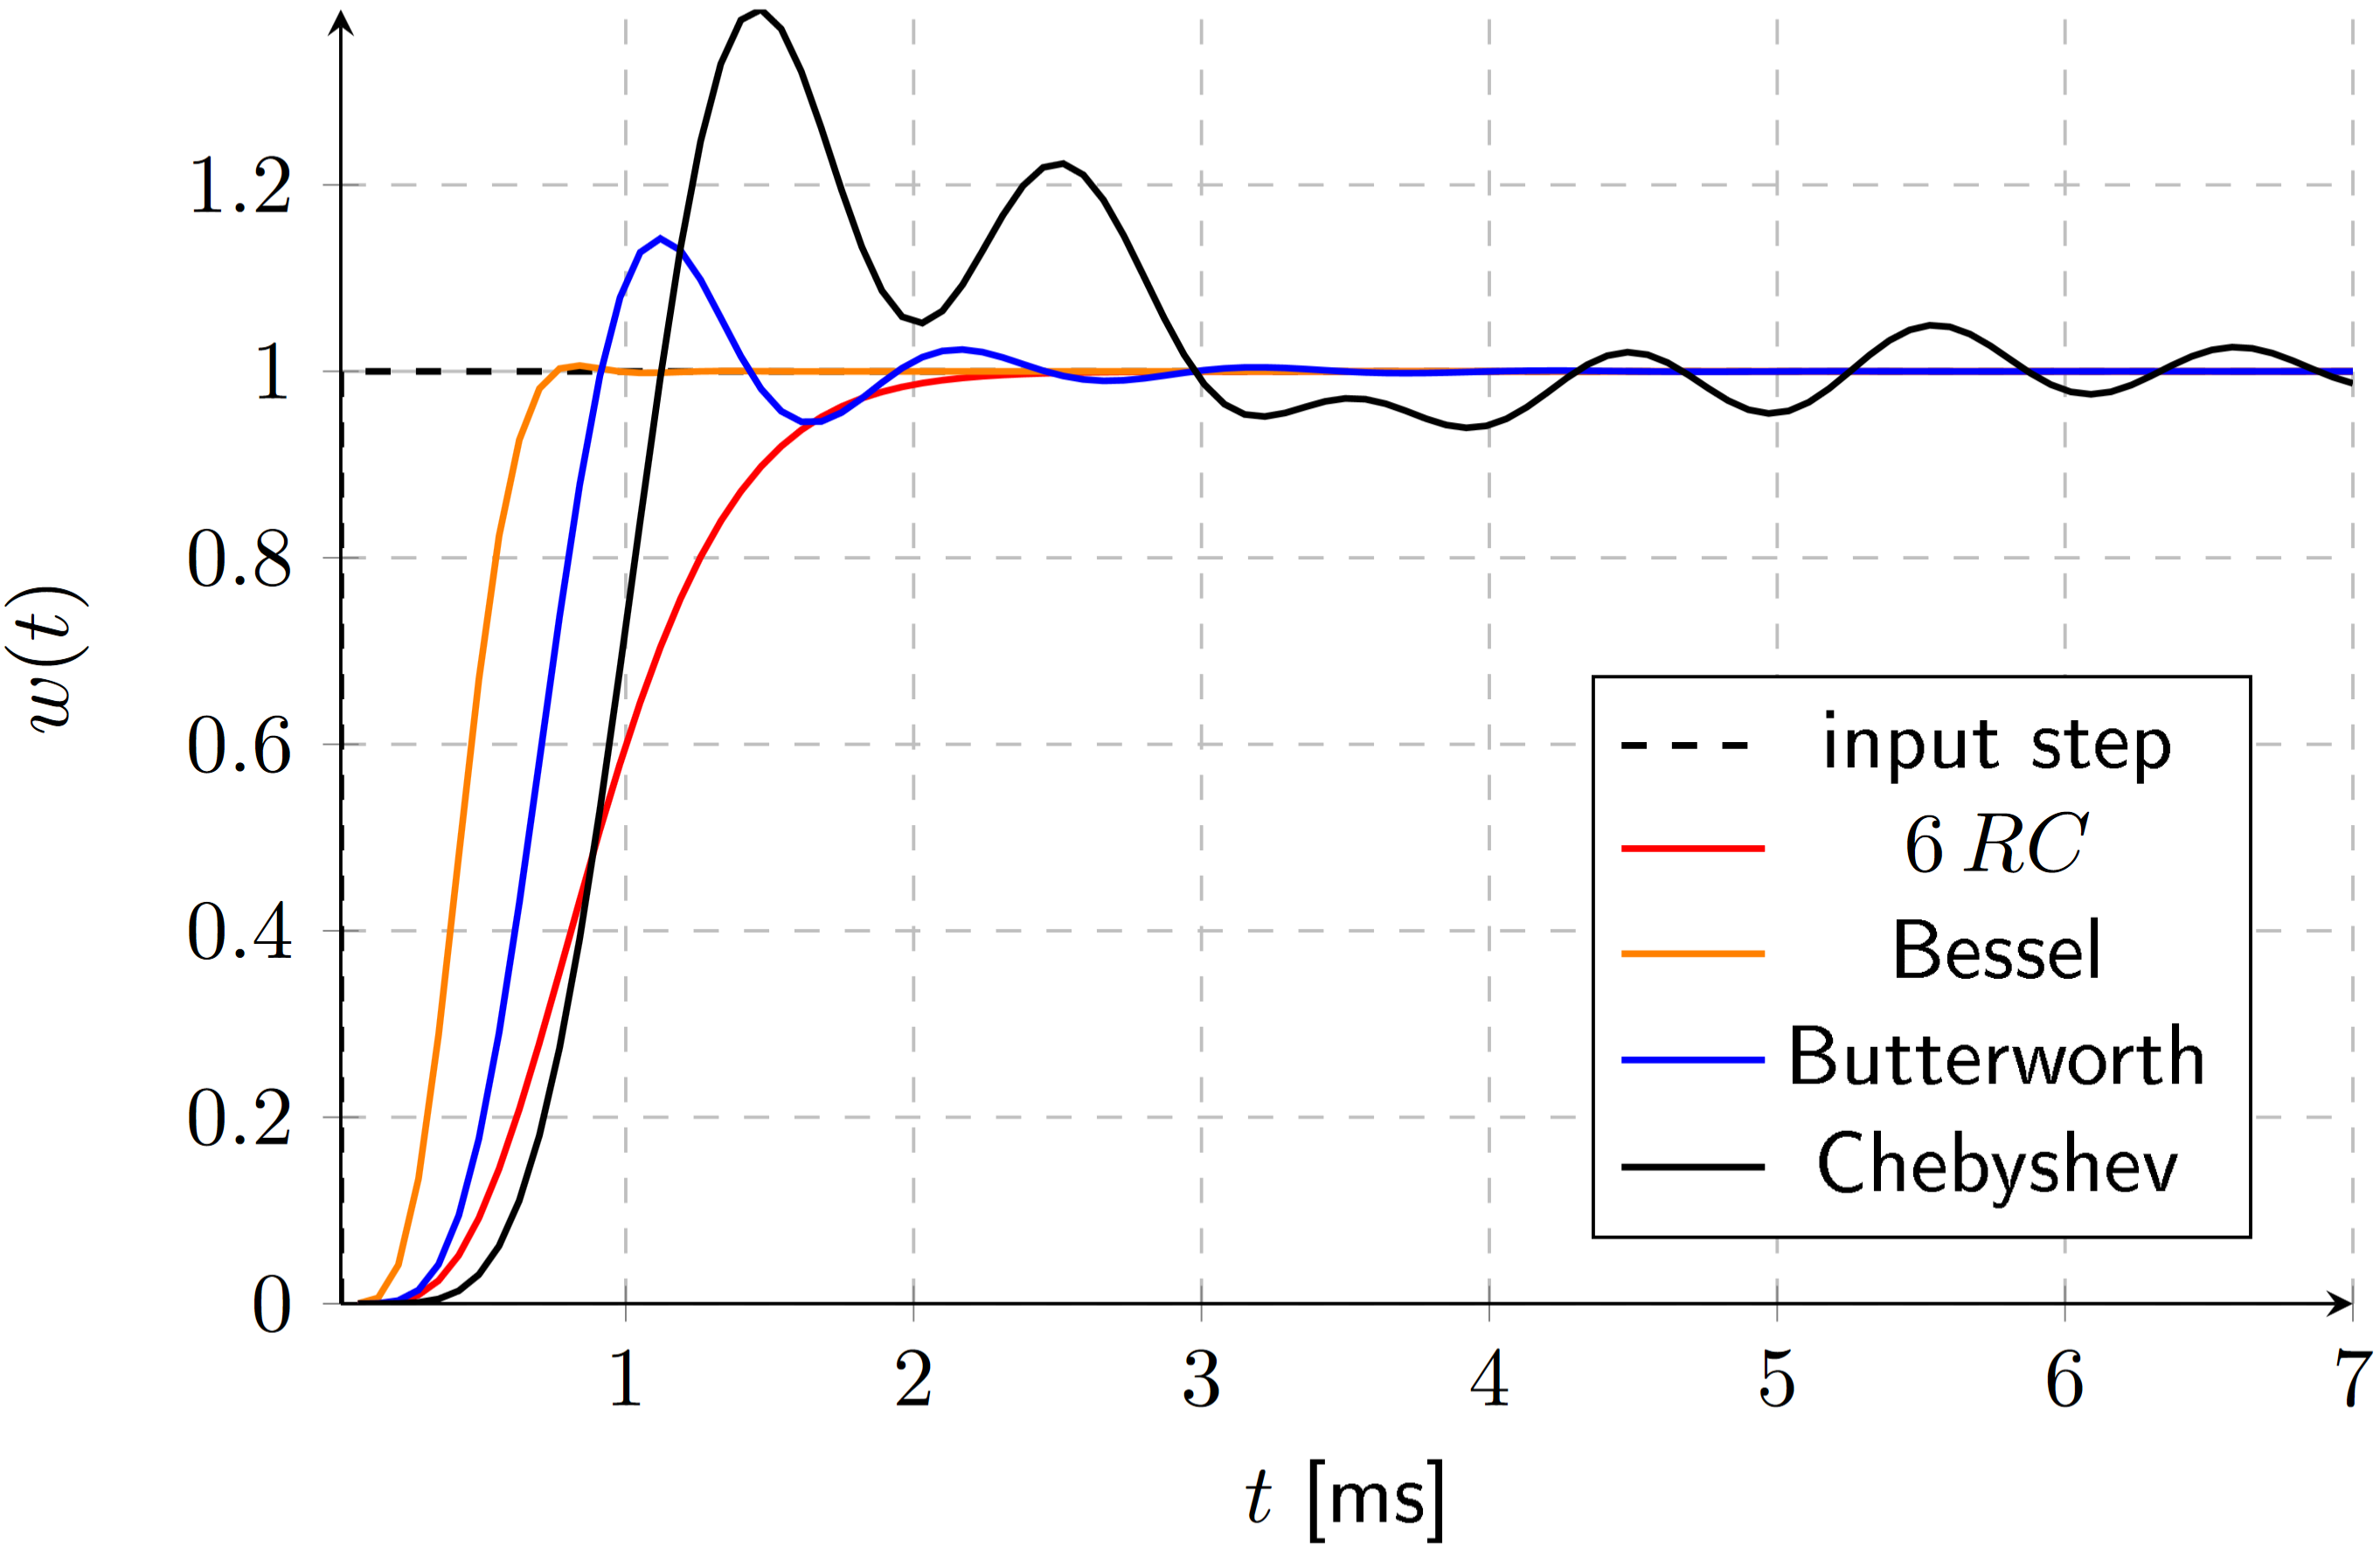
\includegraphics[width=\textwidth]{prechod-porovnani.PNG}
        \caption{Porovnání přechodových charakteristik}
        \label{graf:prechod:porovnani}
    \end{subfigure}
\end{figure}
hmmmmmmmmm\\
 \\
\hrule%-------------------------------------
%\newpage








%6
\section{Nakreslete principiální zapojení zpětnovazební (ZV) struktury a~odvoďte vztah pro výstupní signál. Uveďte základní dělení ZV obvodových struktur a~vliv záporné ZV na vstupní a~výstupní odpor zesilovače}
\subsection*{Principiální zapojení + vztah}
\href[pdfnewwindow=true]{http://hippo.feld.cvut.cz/vyuka/soubory/ElektronickeObvody.pdf#section.10.1}{\textit{Odkaz na odpovídající kapitolu v Hospodkových skriptách}}

\begin{schema}[h!]
    \centering
    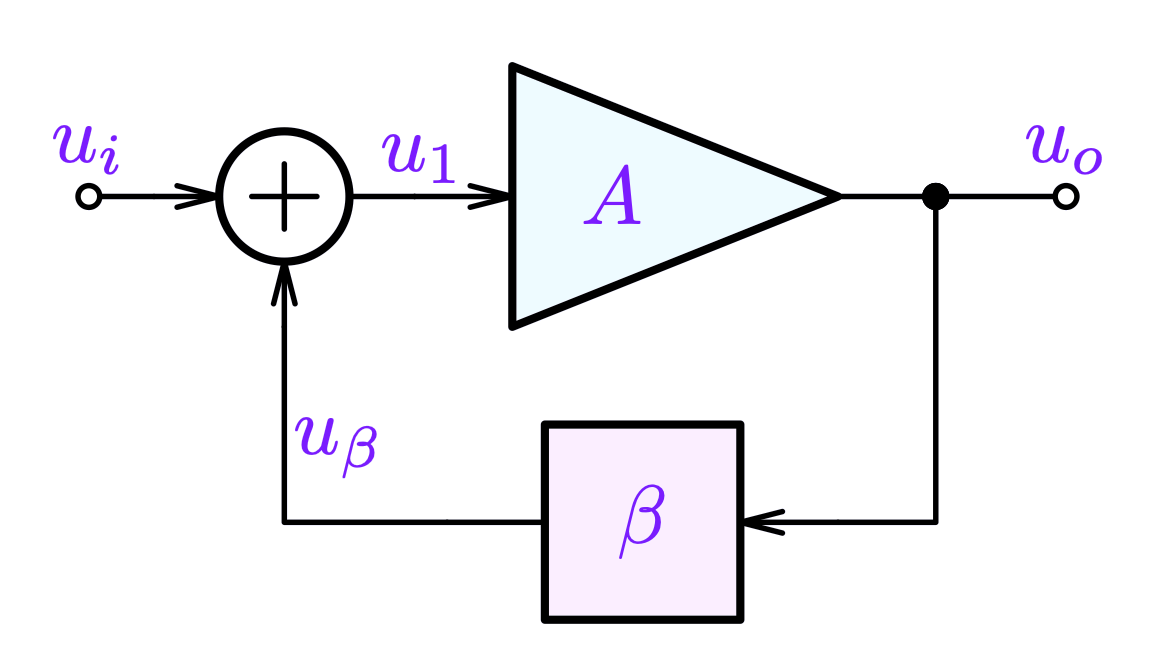
\includegraphics[width=.5\textwidth]{ZV_princip.png}
    \caption{Principiální zapojení ZV systému}
    \label{fig:zv:princip}
\end{schema}

Pro výstup ze sumátoru $u_\text{1}$ platí
\begin{equation*}
    u_\text{1} = u_i + u_\beta.
\end{equation*}
Pro výstup z~bloku $\beta$ resp. vstup do sumátoru $u_\beta$ platí:
\begin{equation*}
    u_\beta = u_o \beta.
\end{equation*}
Pro výstup ze zesilovače se zesílením $A$ platí $u_o = Au_\text{1}$. Dosazením za $u_\text{1}$ dostaneme:
\begin{equation*}
    u_o = (u_i + \beta u_o) = \frac{u_i A}{1-\beta A}.
\end{equation*}

Zesílení soustavy je definováno poměrem výstupu a~vstupu tedy:
\begin{equation}
    \underline{\underline{A' = \frac{u_o}{u_i} = \frac{A}{1-\beta A} = \frac{A}{F}}},
\end{equation}
kde činitel $F = 1-\beta A$ je tzv. \textit{vratným rozdílem} a~činitel $\beta A$ je \textit{přenosem rozpojené ZV smyčky} (signál se zesílí $A$-krát a~pak ještě $\beta$-krát). 

\subsection*{Základní dělení zpětnovazebních obvodových struktur}

\begin{schema}[h!]
    \centering
    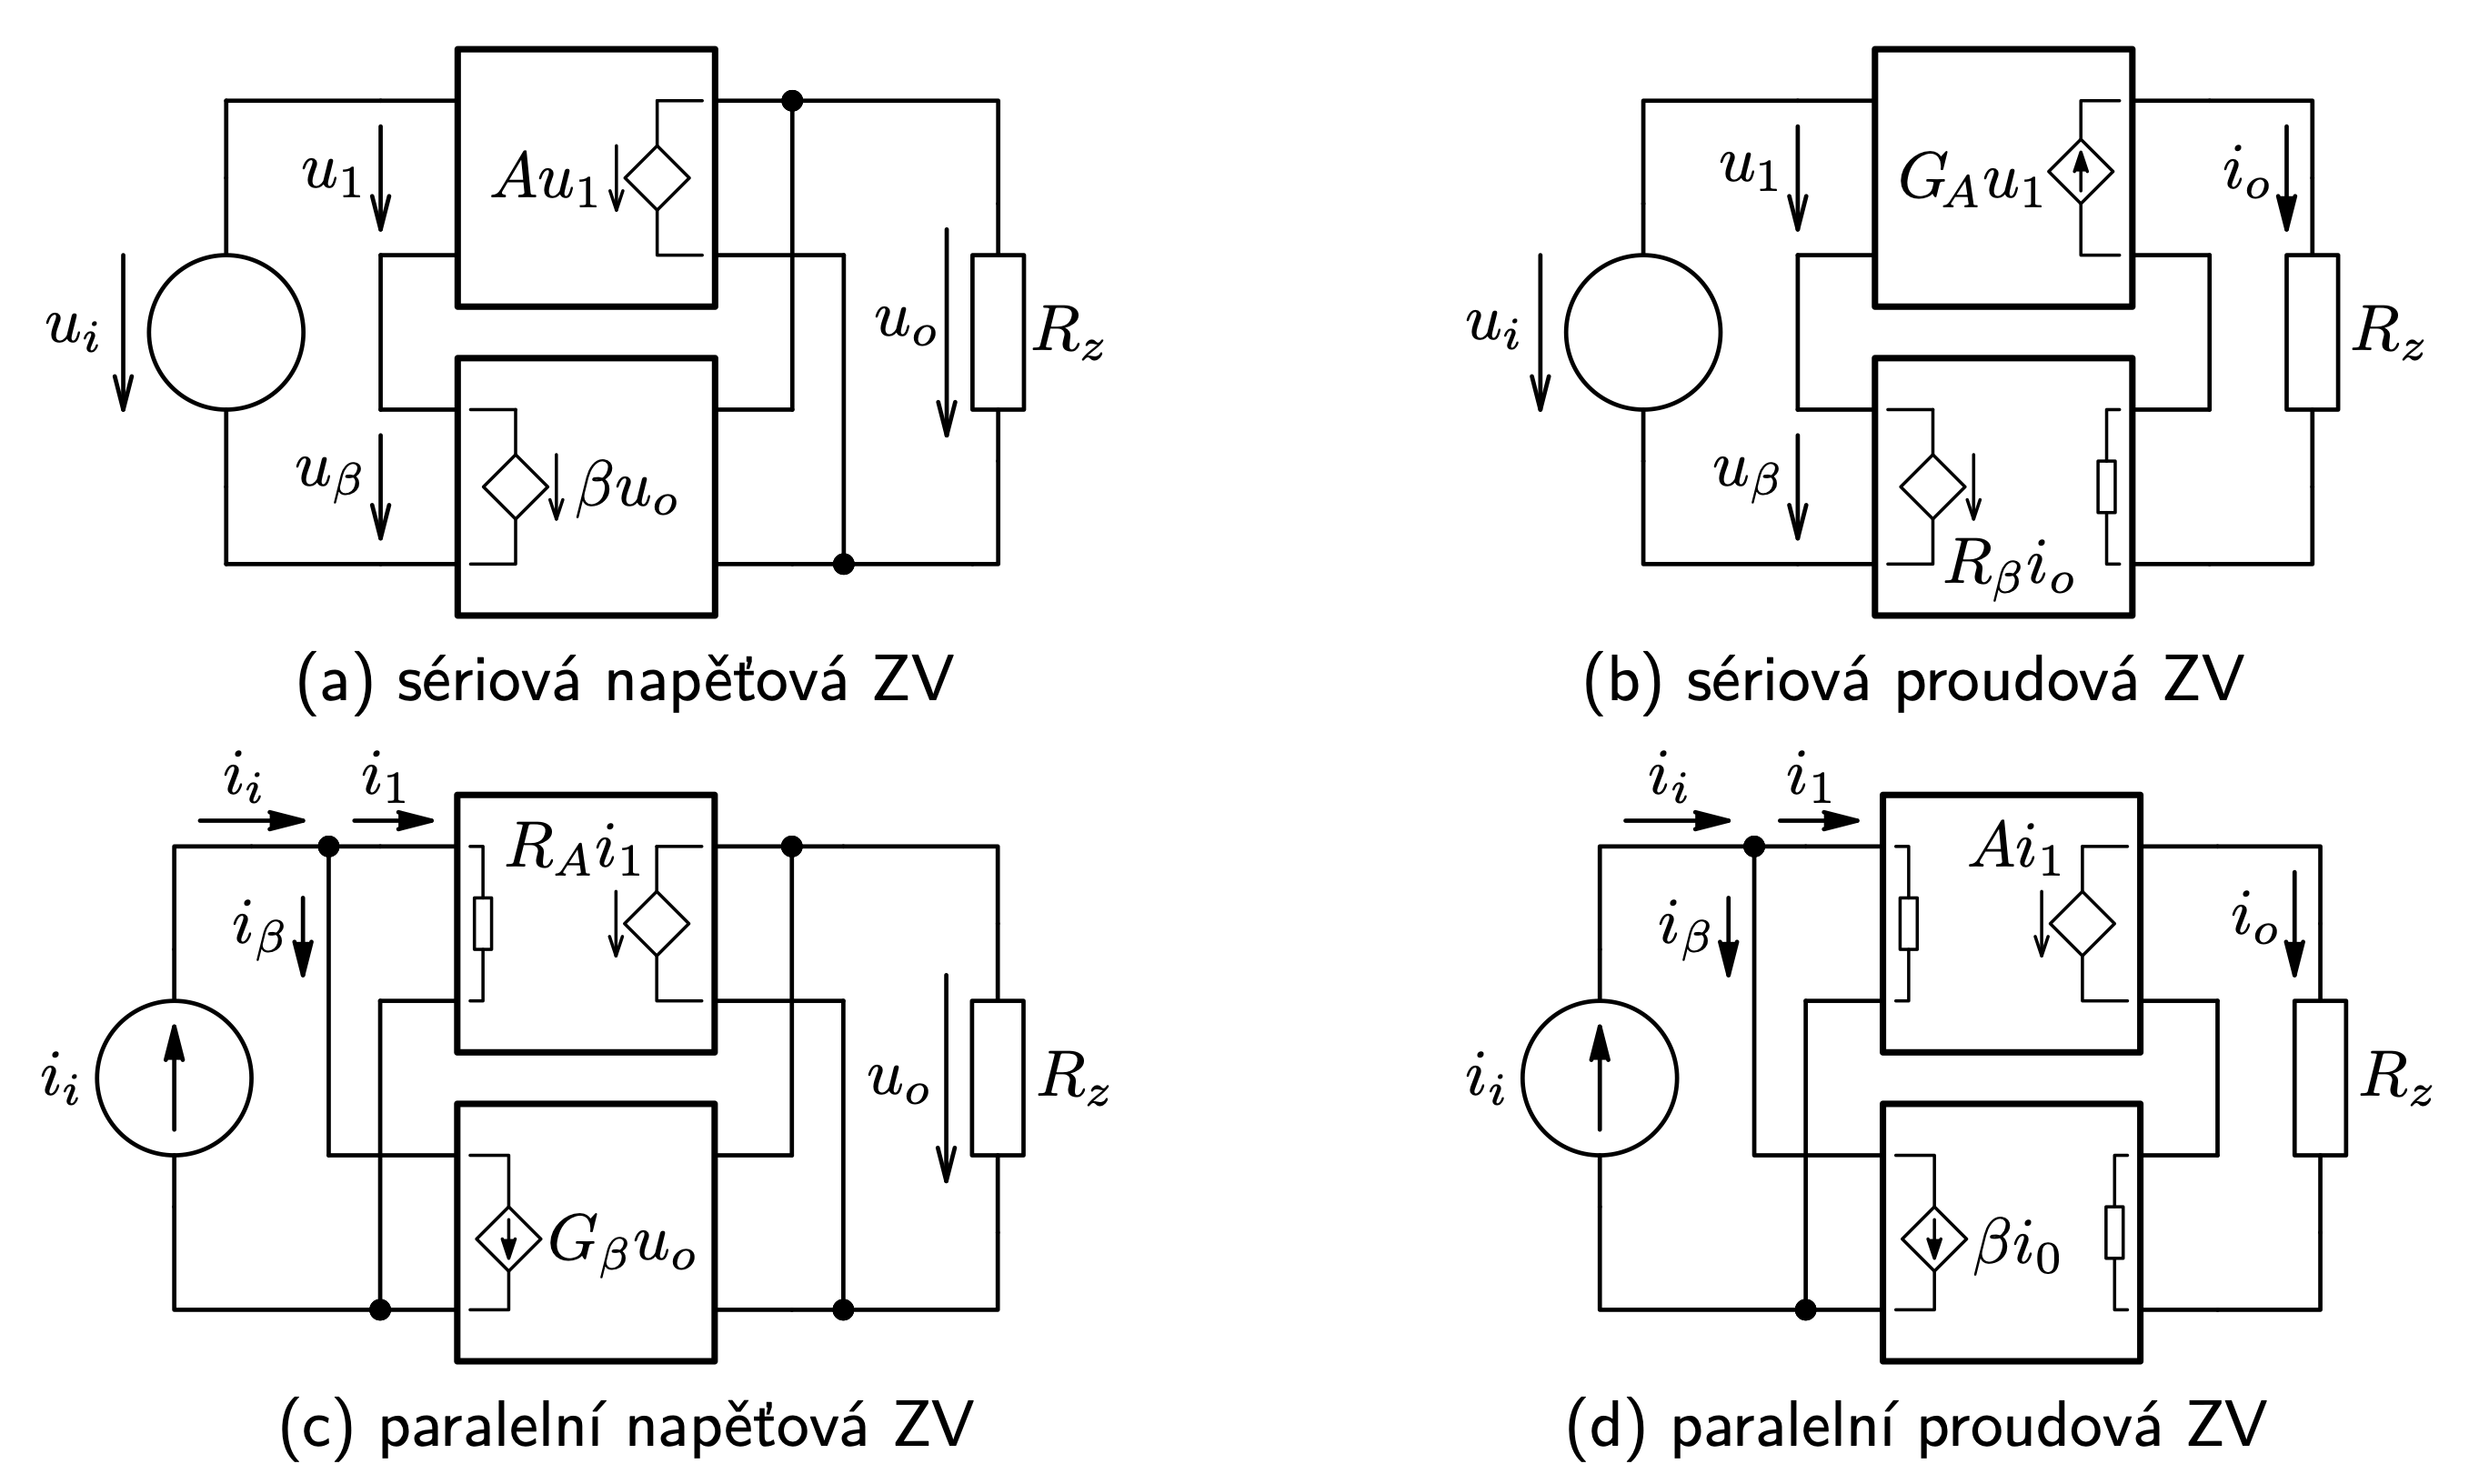
\includegraphics[width=.8\textwidth]{ZV-obvody.png}
    \caption{Dělení ZV podle spojení signálů na vstupu a~dle typu snímaného signálu na výstupu}
    \label{fig:ZV:deleni}
\end{schema}

\textbf{Záporná ZV u operačních zesilovačů}\\
Jestliže se jedná o~\textit{zápornou zpětnou vazbu}, tak buď bude $\beta$ záporná, anebo si ji \uv{zezáporní} zesilovač (např. invertující vstup do operačního zesilovače). Pokud se budeme odkazovat na principiální schéma zpětné vazby viz sch. \ref{fig:zv:princip}, tak $u_1$ - napětí, které se zesiluje (to žije pouze uvnitř toho čipu) je rozdíl napětí na neinvertujícím vstupu $u_i$ a~napětí na invertujícím vstupu $u_\beta$ resp. $u_o\beta$. Z~toho vychází vzoreček pro ZZV.

Jelikož je zpětná vazba vedena do invertujícího vstupu (invertující - \uv{zezáporní} se), platí \textit{Blackův vztah pro ZZV}:
\begin{equation*}
    u_o = u_d\cdot A~= (u_i -\beta u_o) A
\end{equation*}
\begin{equation}
    \underline{\underline{A' = \frac{u_o}{u_i} = \frac{A}{1+\beta A}}}
    \label{eq:vysledne:zesileni}
\end{equation}

\begin{schema}[h!]
    \centering
    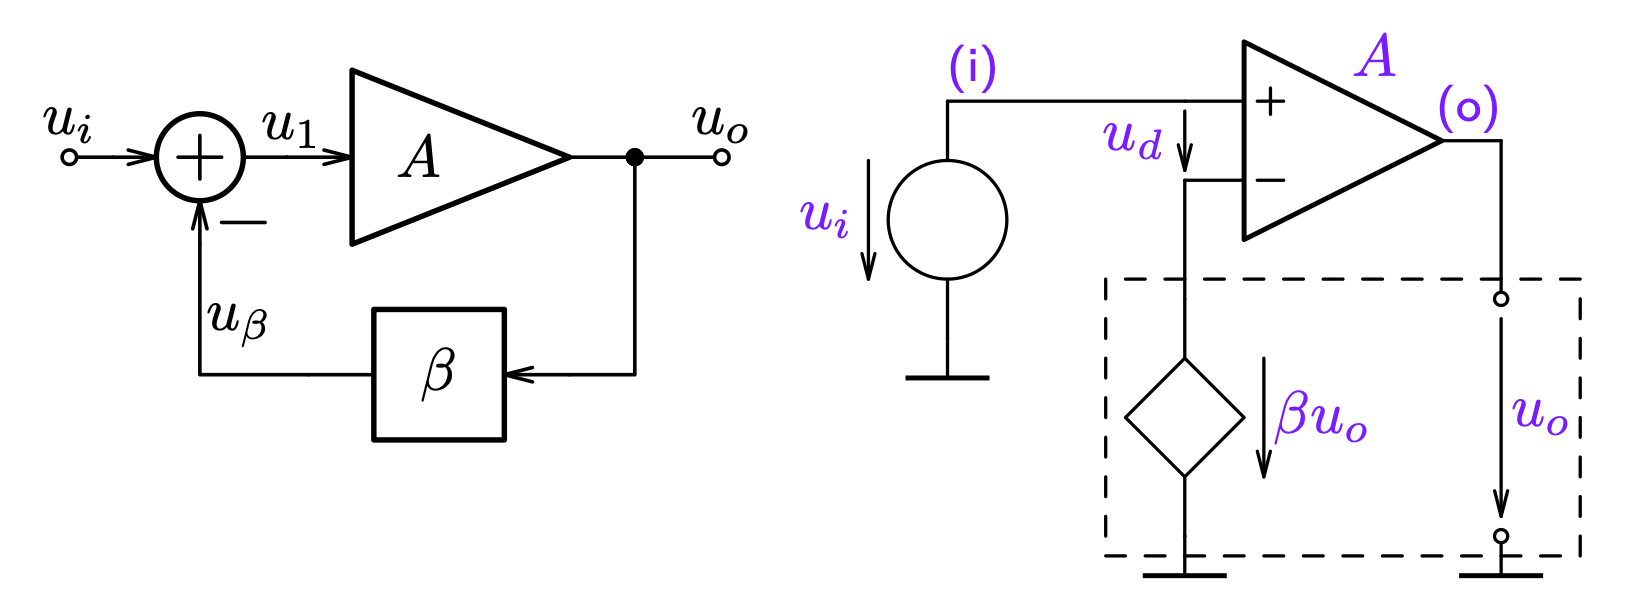
\includegraphics[width=.7\textwidth]{ZZV-OZ.png}
    \caption{Využití záporné zpětné vazby u~zapojení s~operačním zesilovačem}
    \label{fig:opamp:ZZV}
\end{schema}

\textbf{Co je ta beta kurva?} Jak ji mám jako najít v~nějakých načmáraných schématech??

Pokud se podíváme na blokové schéma ZZV ve schématu \ref{fig:opamp:ZZV} níže a~porovnáme se zapojením ve sch. \ref{fig:noninverting}, vidíme jistou podobnost. Na horním obrázku jde do zpětné vazby čtvereček s~betou. Na dolním obrázku je místo čtverečku s~betou dělič napětí, u~kterého můžeme říct, že $\beta = \frac{R_g}{R_f + R_g}$. (Vzoreček pro přenos děliče napětí). AHA! takže už nemusíme myslet abstraktně a~máme v~ruce stavící blok - dělič napětí, který zavedeme do zpětné vazby.

\begin{schema}[h!]
    \centering
    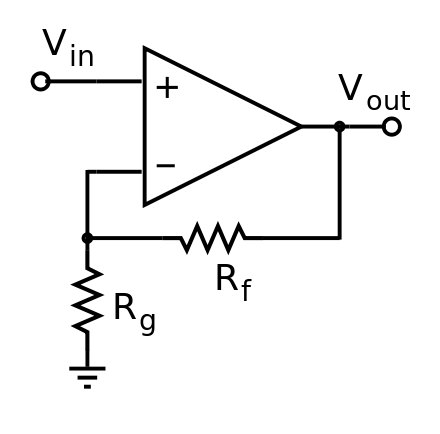
\includegraphics[width=.3\textwidth]{noninverting_opamp.png}
    \caption{Jedno ze dvou nejvíc basic zapojení s~operákem - \textbf{neinvertující zesilovač}}
    \label{fig:noninverting}
\end{schema}

Vnitřní zesílení $A$ operáku (neplést s~$A'$ - zesílení soustavy s přidanou ZZV) může být třeba $10^6$. Pokud vezmeme onen dělič napětí, který bude dejme tomu dvakrát zeslabovat (tedy $R_g = R_f)$, tzn. $\beta = 0.5$, tak po dosazení do Blackova vztahu pro ZZV \eqref{eq:vysledne:zesileni} dostaneme:
\begin{equation*}
    A' = \frac{A}{1+\beta A} = \frac{10^6}{1+0.5\cdot 10^6} \approx \footnote{jedničku ve jmenovateli pošleme v~pizdu, protože vůči milionu je pidi midi} \frac{1}{0.5} = 2 
\end{equation*}

Vzoreček pro neinvertující zesilovač si nechávaj tetovat obvodáři na prsa a~je $A' = 1+\frac{R_f}{R_g}$ .Pokud dosadíme, tak je všecko v~cajku a~sedí oba dva způsoby výpočtu

\subsection*{Vliv ZZV na vstupní a~výstupní odpor}
\textit{Dole je tabulka s~výsledkama}

Budou se tu vyskytovat čtyři veličiny které je potřeba si neplést:
\begin{table}[h!]
    \centering
    \begin{tabular}{ll}
       $R_i$ & vnitřní odpor součástky na vstupu\\
       $R_o$ & vnitřní odpor součástky na výstupu\\
       $R_\text{in}$ & vstupní odpor\\
       $R_\text{out}$ & výstupní odpor\\ 
    \end{tabular}
\end{table}

Vnitřní odpory jsou dány výrobním procesem součástky. Stejně jako baterka má vnitřní odpor i~výstupy čipů mají vnitřní odpor. Vstupní odpor je ale odpor, který vidí signál, když přichází do soustavy a~nelze ho jednoduše změřit ohmmetrem. Jak dále uvidíme, tento odpor je závislý na zesílení soustavy.

\subsubsection*{Vstupní odpor $R_i$ sériové ZV}
Pro sériovou ZV se budeme koukat na schéma \ref{sch:zv:seriova:odpor}.
\begin{schema}[h!]
    \centering
    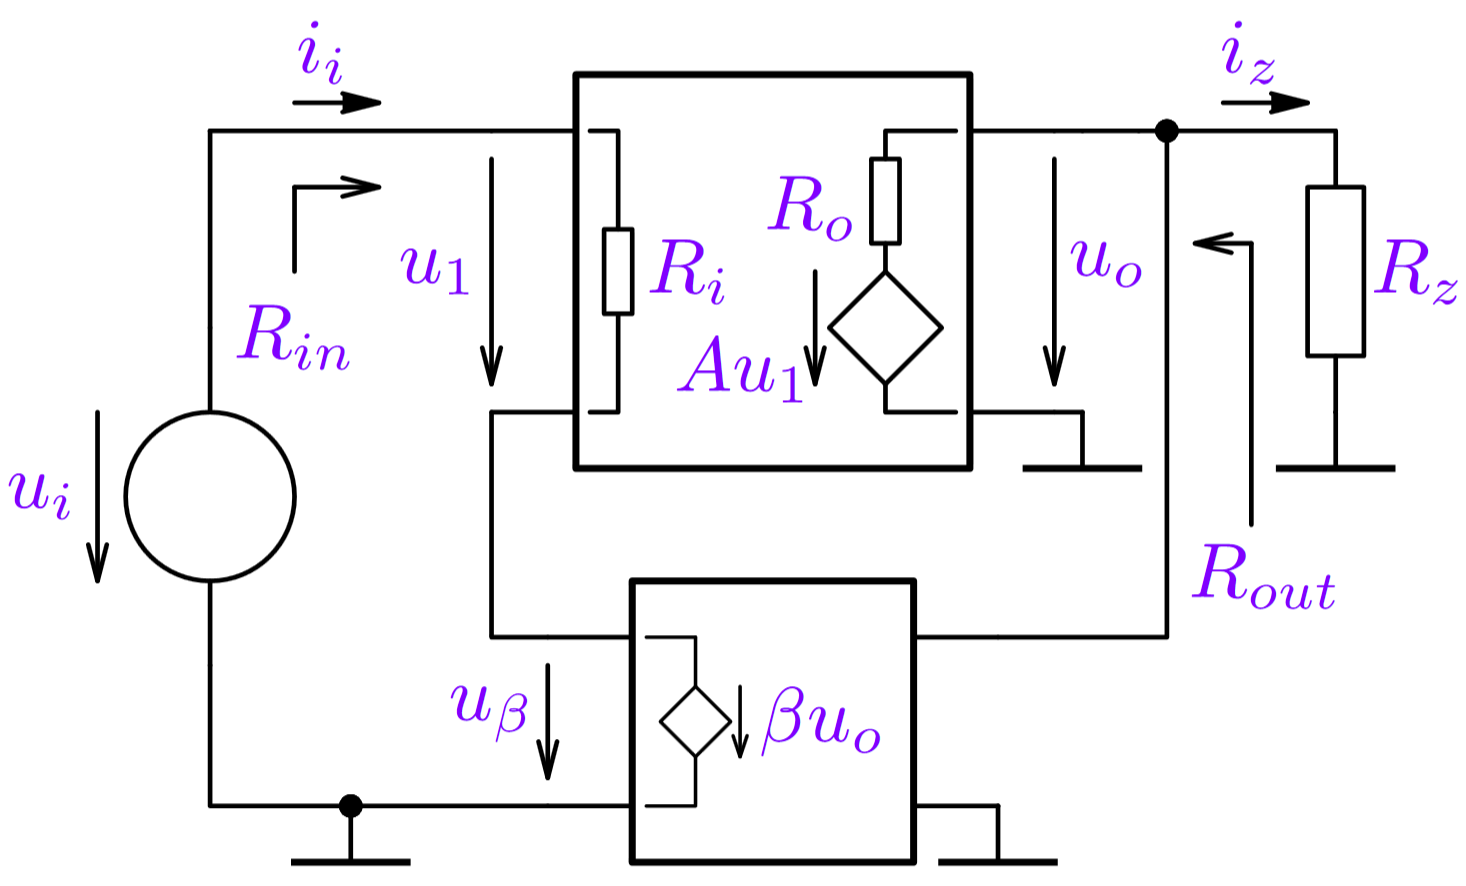
\includegraphics[height=5cm]{ZV_seriova-odpory.PNG}
    \caption{Základní zapojení \textbf{sériové} ZV pro výpočet vstupního a~výstupního odporu}
    \label{sch:zv:seriova:odpor}
\end{schema}

Pár vztahu, které lze vyčíst ze schématu \ref{sch:zv:seriova:odpor} (bereme výstupní odpor $R_o = 0$):
\begin{itemize}
    \item Proud, který teče ze zdroje $u_i$ je stejný jako ten, co protéká skrze $R_i$:
    \begin{equation}
        i_i = i_{Ri} = \frac{u_\text{1}}{R_i}
        \label{eq:ri}
    \end{equation}
    \item Dále platí, že součet napětí $u_\text{1}$ a~$u_\beta$ musí dát $u_i$
    \begin{equation}
        u_i = u_\text{1} + u_\beta
        \label{eq:soucet:napeti}
    \end{equation}
    \item Malý bloček s~betou snímá zprava napětí na $R_z$ resp. výstupní napětí $u_o = Au_\text{1}$. Toto napětí pak zesílí (zeslabí) beta krát a~prdne se doleva jako $u_\beta$:
    \begin{equation}
        u_\beta = \beta u_o = \beta A~u_\text{1}
        \label{eq:beta:napeti}
    \end{equation}
    FAKT BACHA! my tu předpokládáme, že napětí na zátěži $R_z$ je rovno zesílenému $Au_\text{1}$. Tohle jde pouze za předpokladu, že výstupní odpor $R_o = 0$. Zesík nemá výstupní (vnitřní) odpor a~tedy na něm není žádný úbytek napětí.
\end{itemize}


Ohmův vztah praví, že $R=U/I$. Takže vstupní odpor $R_{in}$ jest:
\begin{equation}
    R_{in} = \frac{u_i}{i_i} = \text{viz rovnice \eqref{eq:soucet:napeti} a~\eqref{eq:ri}} = \frac{R_i(u_\text{1}+u_\beta)}{u_1} = \text{viz rce \eqref{eq:beta:napeti}} = \frac{u_\text{1}(1+\beta A)R_i}{u_\text{1}} = \underline{\underline{R_i F}}
\end{equation}

Fuuuuuha, vstupní odpor je dán vnitřním odporem násobeným nějakým zesílením (v našem případě vratným rozdílem $F=(1-\beta A)$. Tohle je velice častá věc a~není blbý si na ni zvyknout.


\subsubsection*{Výstupní odpor $R_o$ sériové ZV}

Resetujeme mozek a~opět uvažujeme, že vnitřní odpor na výstupu $R_o$ existuje a~má nějakou hodnotu.

Výstupní odpor se určí sloganem \textit{napětí na prázdno lomeno proud nakrátko}. 

Napětí naprázdno je (\textit{zkuste odvodit}):
\begin{align*}
    u_o = \frac{u_i A}{1+\beta A}
\end{align*}

Proud nakrátko je
\begin{equation*}
    i_z = \frac{A u_i}{R_o}
\end{equation*}

Dosadíme do sloganu pro výpočet výstupního odporu a~máme
\begin{equation}
    R_{out} = \frac{u_o}{i_z} = \frac{R_o \cancel{u_i A}}{\cancel{u_i A}(1+\beta A)} = \underline{\underline{\frac{R_o}{F}}}
\end{equation}

\subsubsection*{Vstupní odpor $R_i$ paralelní ZV}
Pro paralelní ZV se budeme koukat na schéma \ref{sch:zv:paralelni:odpor}.
\begin{schema}[h!]
    \centering
    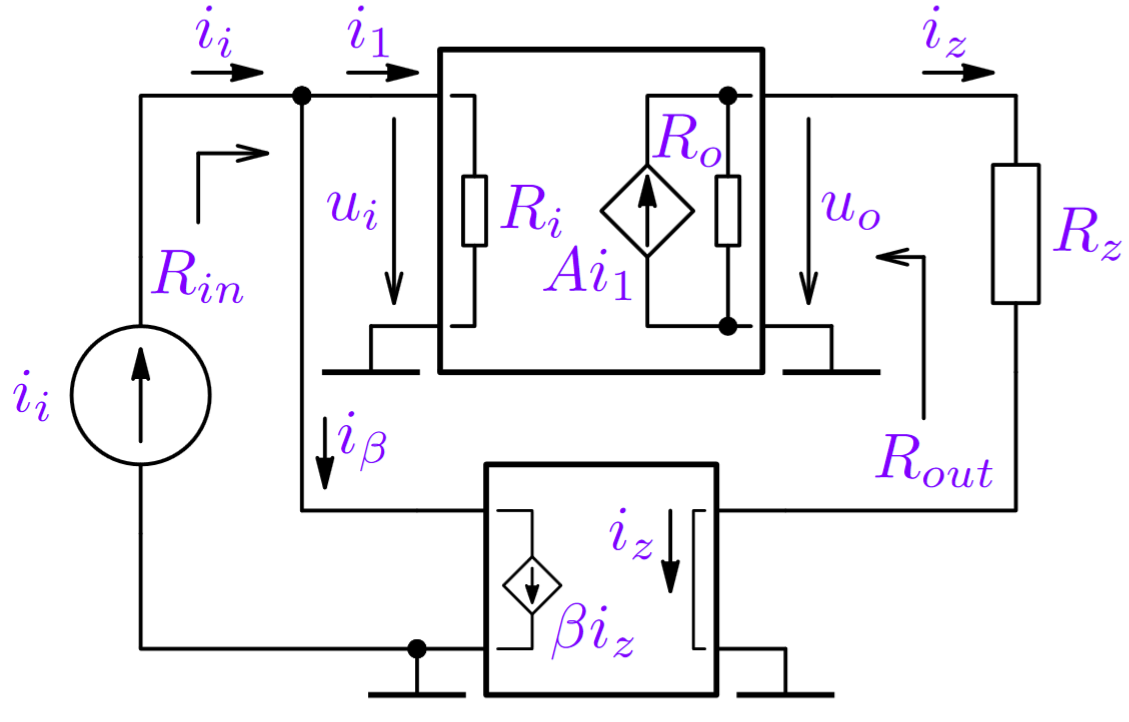
\includegraphics[height=5cm]{ZV_paralelni-odpory.PNG}
    \caption{Základní zapojení \textbf{paralelní} ZV pro výpočet vstupního a~výstupního odporu}
    \label{sch:zv:paralelni:odpor}
\end{schema}

Už to vezmeme letem světem. V~tomto případě je na výstupu proudový zdroj. Abychom si zjednodušili život, tak $R_o \rightarrow \infty$, takže proud tvořený zdrojem (kosočtverec vpravo na výstupu zesilovače) poteče všechem do zátěže. Pak platí: 
\begin{equation}
    u_i = u_\text{1} R_i,~~~~i_i=i_\text{1} + i_\beta,~~~~ i_\beta = \beta i_z = \beta i_1 A
\end{equation}

\begin{equation}
    R_{in} = \frac{u_i}{i_i} = \dots = \underline{\underline{\frac{R_i}{F}}}
\end{equation}

\subsubsection*{Výstupní odpor $R_i$ paralelní ZV}
Výstupní odpor určíme opět sloganem \textit{napětí na prázdno lomeno proud nakrátko}.
Pokud pošleme zátěž $R_z$ v~pizdu (odborně se tomu říká $R_z \rightarrow \infty$), můžeme psát:
\begin{equation*}
    u_o = Ai_\text{1}R_o = Ai_iR_o
\end{equation*}
Pro tento případ se $i_i = i_\text{1}$. To proto, že jsme odebrali $R_z$ a~tedy nic neteče do zpětné vazby a~$i_\beta = 0$

Proud na krátko získáme proklemováním (přemostěním) $R_z$. Před Hospodkou budeme říkat $R_z = 0$. Pak platí:
\begin{equation*}
    i_z = \frac{i_i A}{1+\beta A}
\end{equation*}

Výstupní odpor $R_{out}$ pak získáme jako
\begin{equation}
    R_{out} = \frac{napeti~naprazdno}{proud~nakratko} = \frac{u_o}{i_z} = \dots = \underline{\underline{R_o F}},
\end{equation}
kde $F=1+\beta A$

Suma sumárum máme tuhletu tabulku:
\begin{table}[h!]
    \centering
    \begin{tabular}{|l|c|c|}
        \hline
        & Sériová ZV & Paralelní ZV\\\hline\hline
        \rule{0pt}{2.5ex}Vstupní odpor & $Z_{in} = Z_i F$ & $R_{in} = \frac{R_i}{F}$\\[.7ex]\hline
        \rule{0pt}{2.5ex}Výstupní odpor & $Y_{out} = \frac{R_o}{F}$ & $R_{out} = R_o F$\\[.7ex]\hline
    \end{tabular}        
    \caption{Výsledné odpory pro daná zapojení, $F=1+\beta A$}
\end{table}%

Pokud chceme být jooo cool lidi, tak můžeme začít házet slova jako impedance a~admitance. To se hodí v~případě střídavých signálů a~vstupní a~výstupní impedance jsou poté:
\begin{table}[h!]
    \centering
    \begin{tabular}{|l|l|}
        \hline
        \multicolumn{1}{|c|}{Sériová ZV }& \multicolumn{1}{|c|}{Paralelní ZV}\\\hline\hline
        Vstupní impedance: $Z_{in} = Z_i F$ & Vstupní admitance: $Y_{in} = Y_i F$\\\hline
        Výstupní admitance $Y_{out} = Y_o F$ & Výstupní impedance $Z_{out} = Z_o F$\\\hline
    \end{tabular}
    \caption{Výsledné impedance a~admitance pro daná zapojení, $F=1+\beta A$, $Z_i = \frac{1}{Y_i}$ a~$Z_o = \frac{1}{Y_o}$ pro $A=0$}
\end{table}%










%7
\section{Jak se zajišťuje stabilita ZV soustav a~co musí platit pro stabilní systém? Vysvětlete pojem „fázová jistota“ a~„doplňkový zisk“. Co je to kmitočtová kompenzace zesilovače a~proč se používá?}
\href[pdfnewwindow=true]{http://hippo.feld.cvut.cz/vyuka/soubory/ElektronickeObvody.pdf#subsection.10.8.4}{\textit{Odkaz na odpovídající kapitolu v Hospodkových skriptách}}

\subsection*{Stabilita zpětnovazebné soustay - co zajišťuje \& podmínky}
Stabilita se ověřuje v~tzv. open loop zapojení - zapojení s~rozpojenou zpětnovazební smyčkou viz schéma \ref{sch:zv:open:loop}. Zatěžovací odpor $R_z$ je dán zapojením ZV (sériová/paralelní), vstupním odporem a~vnitřním odporem zesilovače.
\begin{figure}[h!]
    \centering
    \begin{subfigure}{.45\textwidth}
        \centering
        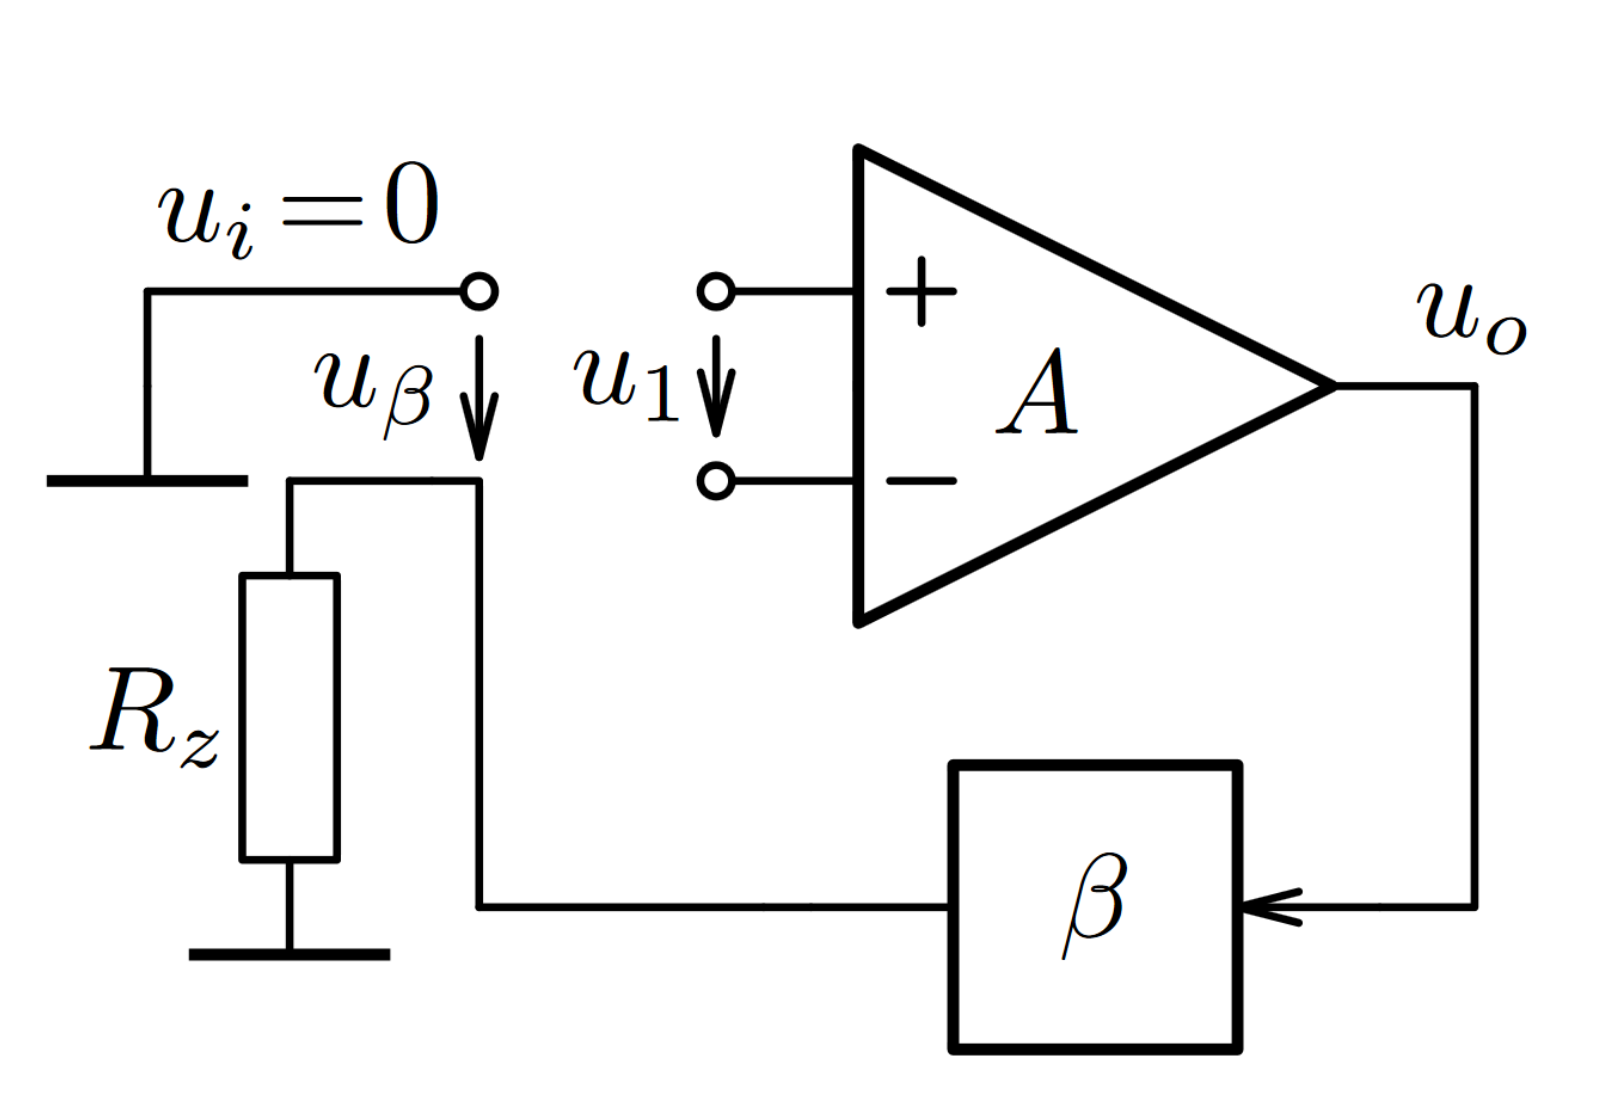
\includegraphics[width=\textwidth]{ZV-open_loop.PNG}
        \caption{Určení přenosu rozpojené ZV smyčky}
        \label{sch:zv:open:loop}
    \end{subfigure}
    \begin{subfigure}{.45\textwidth}
        \centering
        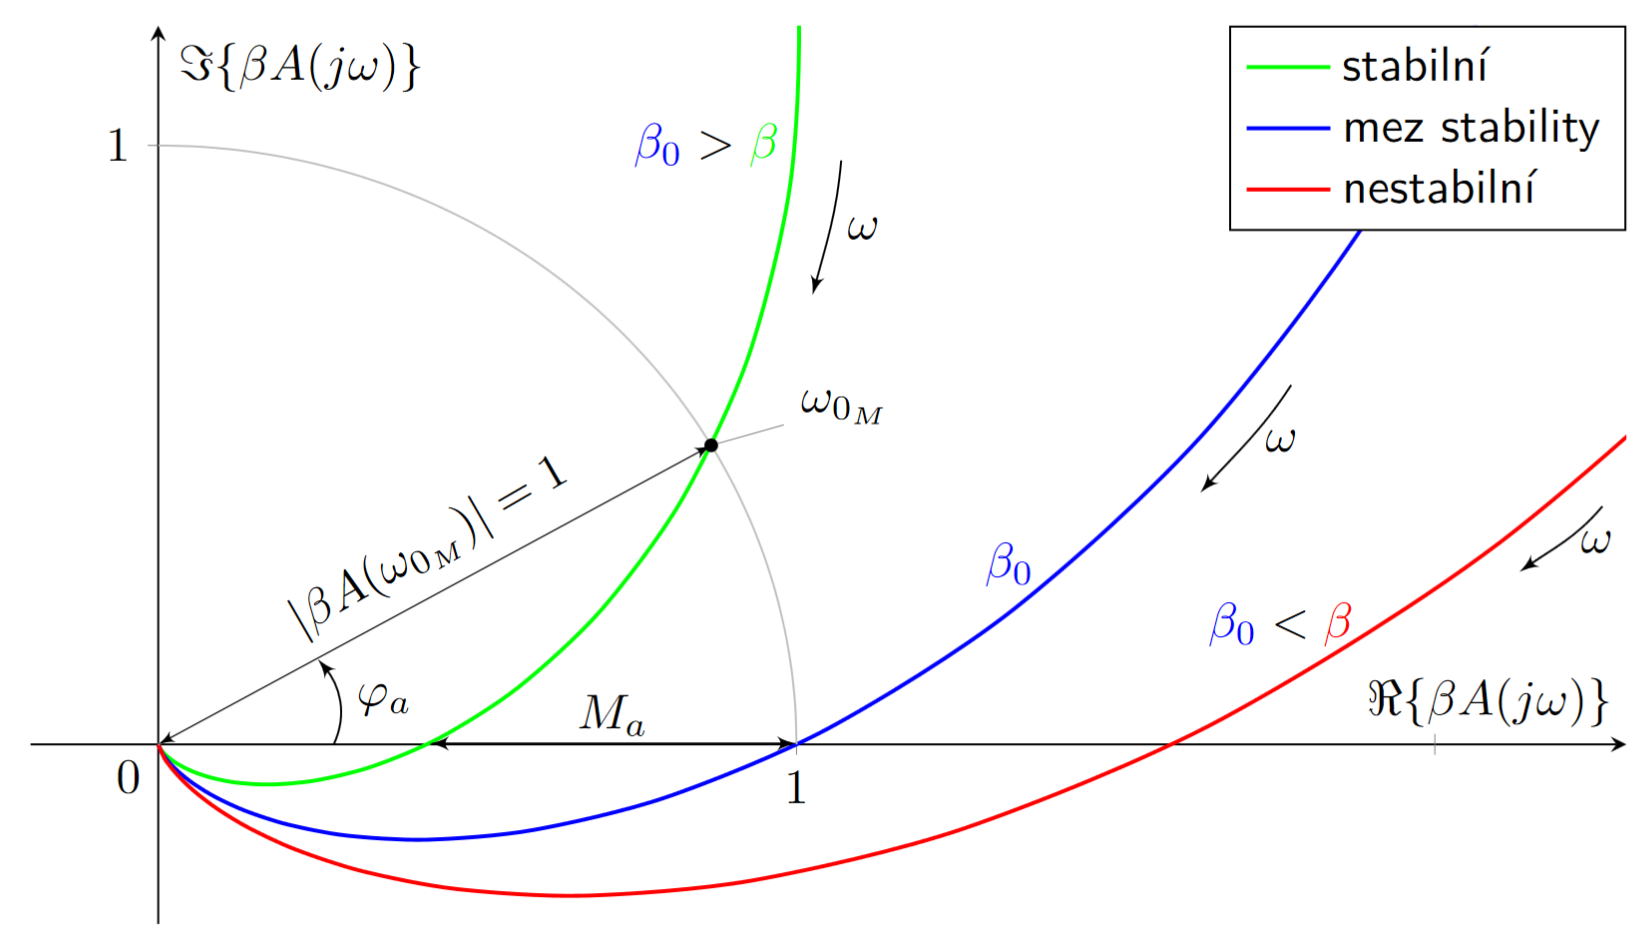
\includegraphics[width=\textwidth]{stabilita_vice.PNG}
        \caption{Kmitočtové charakteristiky pro různé hodnoty $\beta$}
        \label{graf:stabilita}
    \end{subfigure}
    \caption{Zjišťování stability ZV soustav}
\end{figure}

\begin{table}[h!]
    \centering
    \begin{tabular}{rl}
        $\beta A~< 0 (F>1)$ & stabilní záporná ZV\\
        $\beta A~= 0 (F=0)$ & obvod bez vazby \\
        $0 < \beta A~< 1(1>F>0)$&stabilní kladná vazba\\
        $\beta A~= 1 (F=0)$ & mez stability, obvod kmitá\\
    \end{tabular}
    \caption{Stabilita pro různé činitele $\beta A$ resp. vrazný rozdíl $F$}
    \label{tab:stabilita}
\end{table}
% Pro kmitočtově závislé obvody je $\beta A$ kmitočtově závislá a~tedy podle posledního řádku tabulky \ref{tab:stabilita} musí platit
% \begin{equation*}
%     |\beta A(\omega_{0_M})| = 1
% \end{equation*}

\subsection*{Fázová jistota a~doplňkový zisk}
Abychom zajistili stabilitu systému, tak kmitočtová charakteristika viz graf \ref{graf:stabilita} by měla protnout jednotkovou kružnici lehce nad reálnou osou. Jak je vidět v~grafu, úhel $\varphi_a = 30~\degree$ a~nazývá se fázová jistota. Jde o~bod, kde $|\beta A(\omega_{0_M})| = 1$ a~tedy $\varphi_{\beta A}(\omega_{0_M}) = \varphi_a > 30~\degree$.

\textbf{Lidsky}: kmitočet $\omega_{0_M}$ je právě ten, při kterém charakteristika protne jednotkovou kružnici a~tento průnik by měl svírat úhel větší jak $30~\degree$

\textbf{Doplňkový zisk} je poté definován jako
\begin{equation*}
    M_a = 1-|\beta A(\omega_{0_\varphi})| > 10~\text{dB}.
\end{equation*}
Jedná se o~vzdálenost mezi jedničkou a~bodem, kde protíná zelená charakteristika reálnou osu.

Přenos skrze zesilovač a~zpětnou vazbu bude následně
\begin{equation*}
    A' = \beta A~= \frac{u_\beta}{u_\text{1}} = \frac{U_\beta (s)}{U_\text{1}(s)}
\end{equation*}

\subsection*{Kmitočtová kompenzace}
Při zesilování střídavého napětí se směrem k~vyšším kmitočtům snižuje zesílení a~mění fáze signálu. To bývá příčinou nestability. Pokud se totiž fáze změní až o~$180~\degree$, změní se původně záporná zpětná vazba na kladnou a~OZ se rozkmitá. Proto se zavádí kmitočtová kompenzace.

Jde o~techniku \textbf{přidání dominantního pólu}, aby byla soustava stabilní i~pro vysoké kmitočty, při kterých by jinak docházelo k~obracení fáze rozpojené zpětnovazební smyčky.








\newpage
%8
\section{Nakreslete invertující a~neinvertující zesilovače s~OZ a~odvoďte vztah pro napěťové zesílení v~případě ideálního OZ. Jaký je vstupní odpor zapojení?}
\href[pdfnewwindow=true]{http://hippo.feld.cvut.cz/vyuka/soubory/ElektronickeObvody.pdf#section.11.3}{\textit{Odkaz na odpovídající kapitolu v Hospodkových skriptách}}

\textbf{Motivace}: důležitá věc pro praxi, tohle je fakt dobrý mít zmáknutý.
\begin{figure}[h!]
    \centering
    \begin{subfigure}{.5\textwidth}
        \centering
        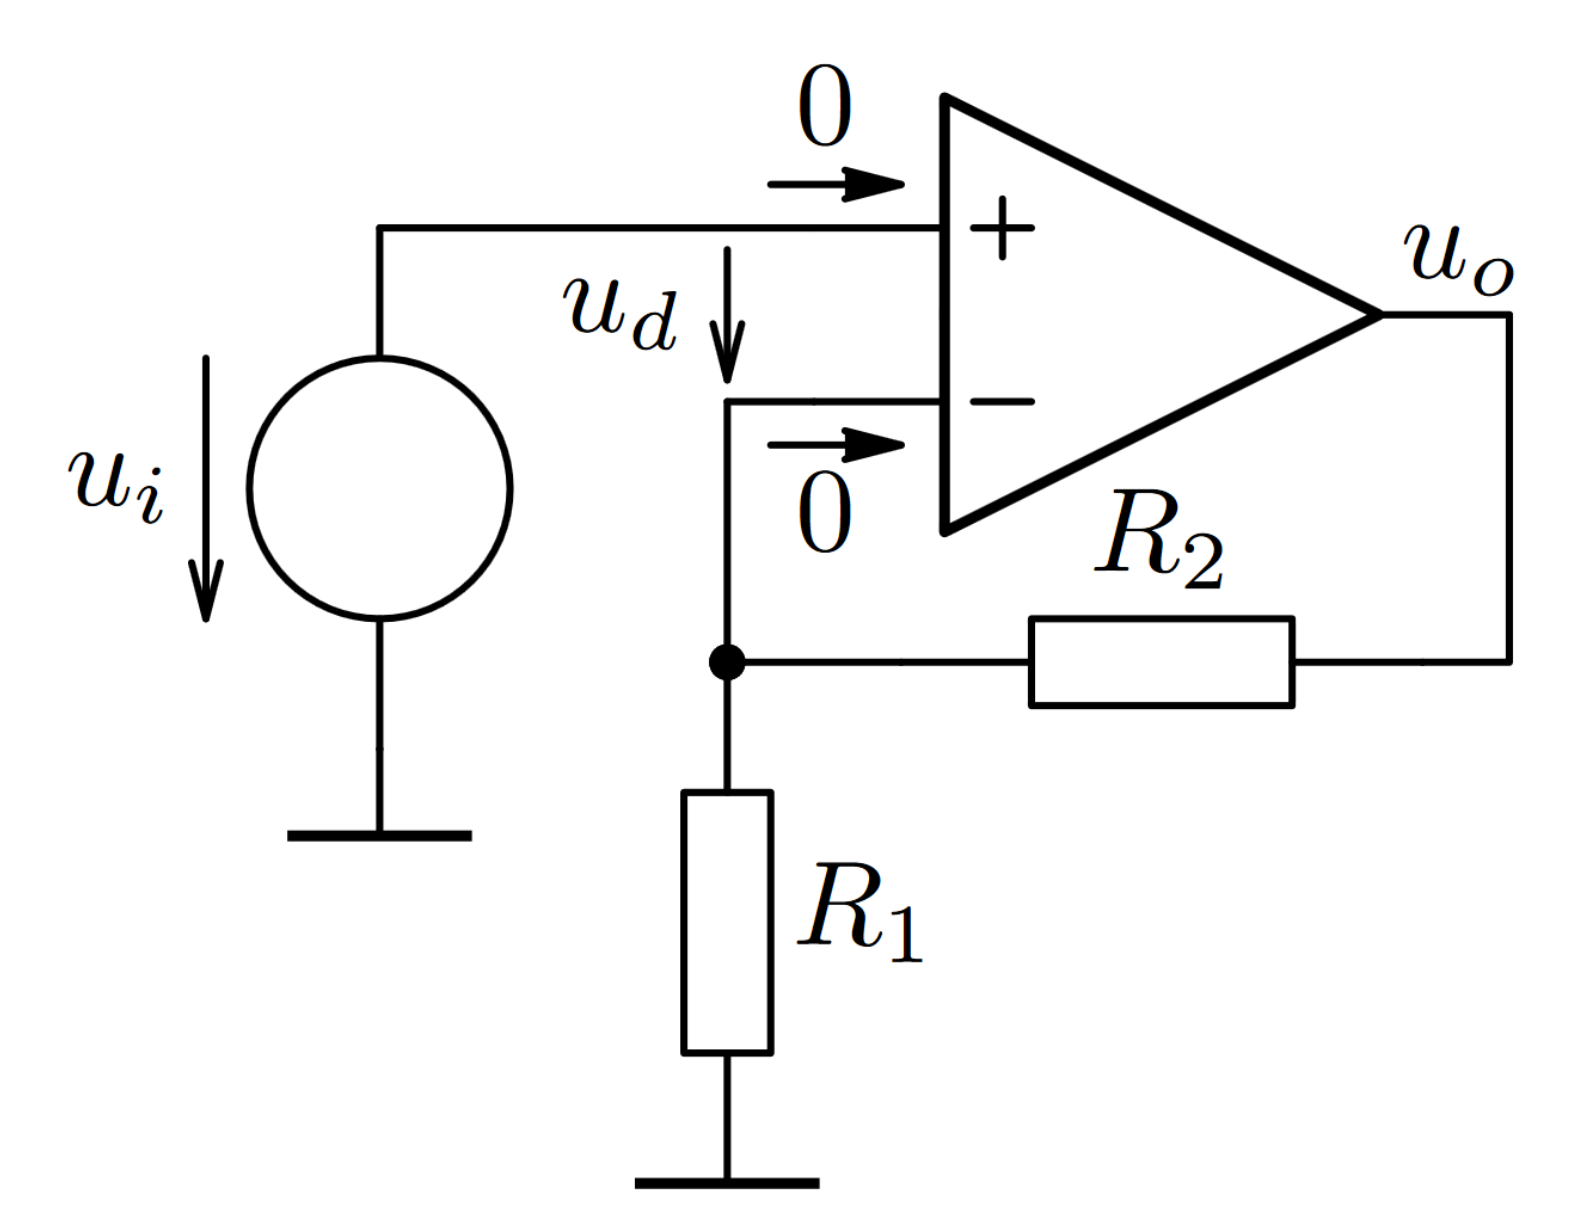
\includegraphics[height=.6\linewidth]{opamp-noninvert.PNG}
        \caption{Neinvertující zesilovač}
    \end{subfigure}%
    \begin{subfigure}{.5\textwidth}
        \centering
        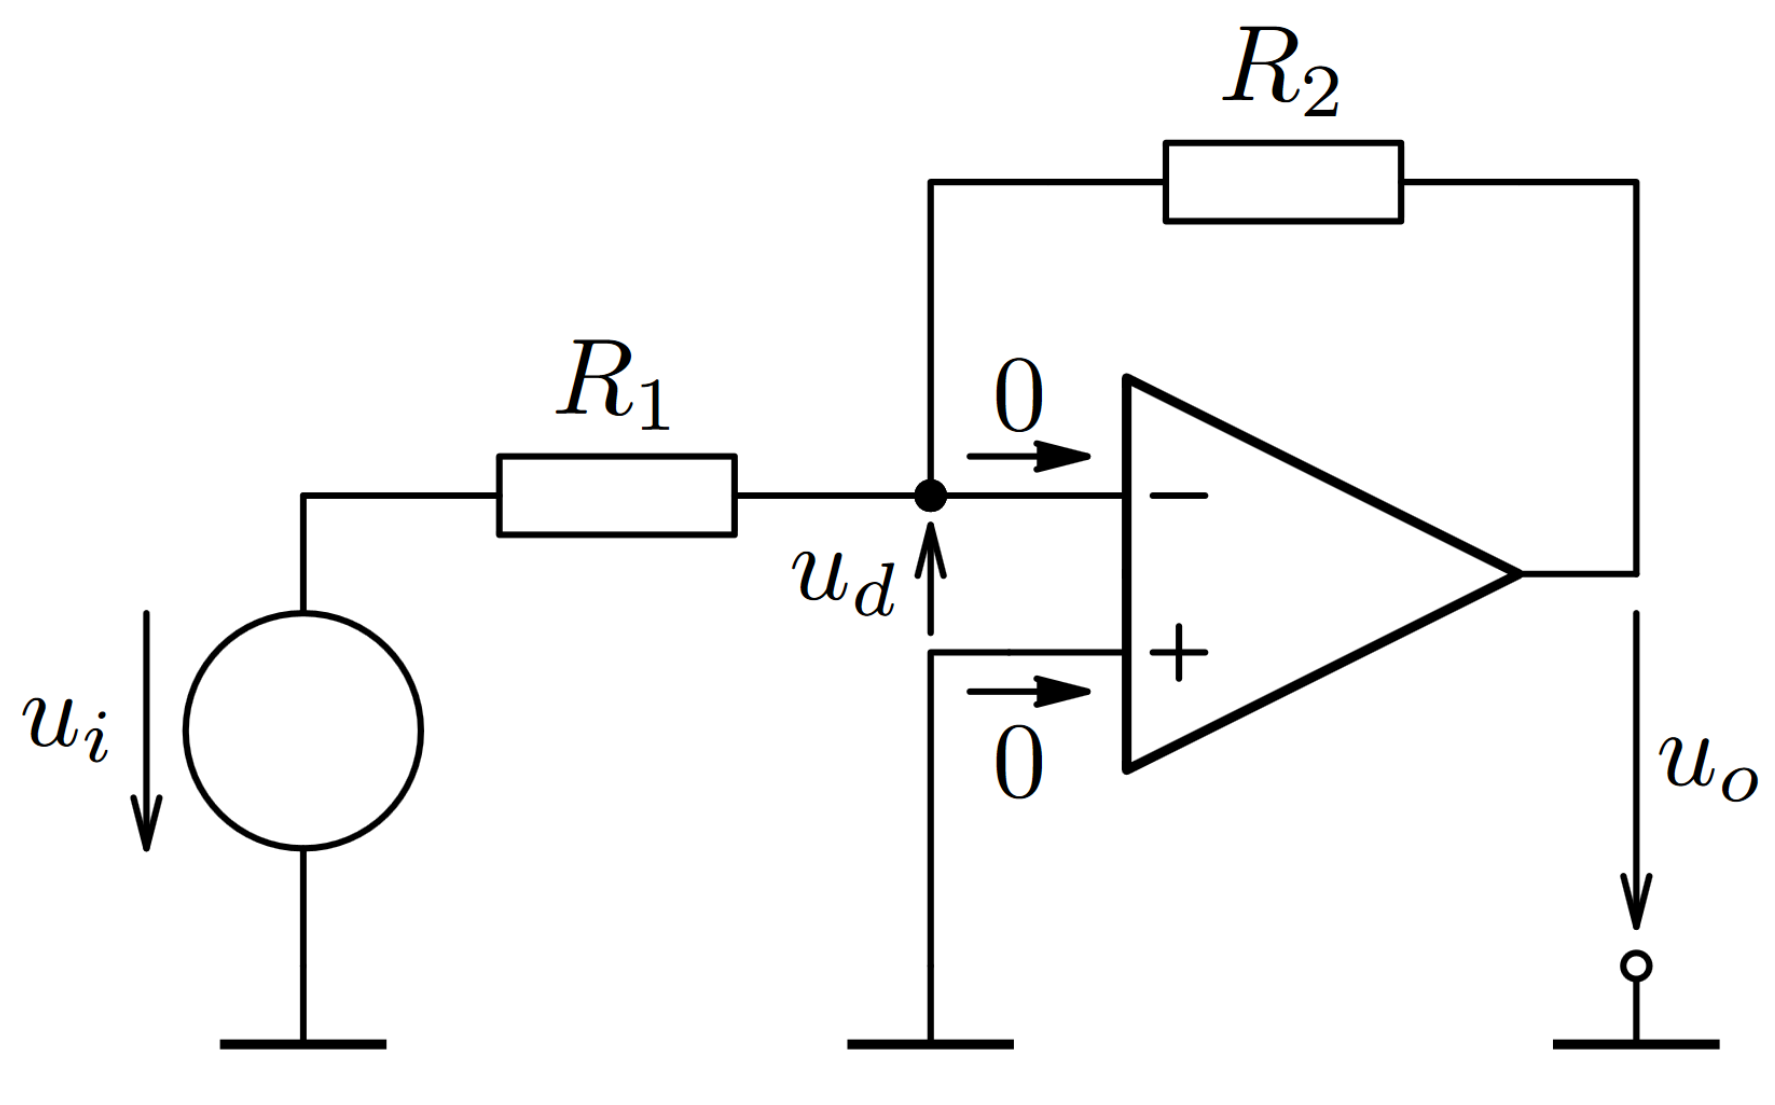
\includegraphics[height=.6\linewidth]{opamp-invert.PNG}
        \caption{Invertující zesilovač}
    \end{subfigure}
    \caption{Dvě úplně nějvíc basic zapojení zesilovačů s~operákama}
    \label{fig:operaky}
\end{figure}

\subsection*{Odvození vztahu}
Dvě MEGAMEGAMEGAmoc důležité mantry:
\begin{enumerate}
    \item Pokud se k~operáku chováme hezky, tak si výstup řídí tak, aby na vstupu byla \textbf{stejná napětí}
    \item Do vstupů operáku \textbf{neteče žádný proud}
\end{enumerate}

S tímto se můžeme vydat do světa odvozování. Začněme s~neinvetujícím zesilovačem:\\
Na neinvertujícím (+) vstupu je napětí $u_i$. Mantra říká, že i~na invertujícím (-) vstupu bude $u_i$. Napětí $u_i$ bude i~na výstupu děliče napětí, tvořeného rezistory $R_1$ a~$R_2$. To nám dává do ruky následující vztah:
\begin{equation*}
    u_i = u_o \frac{R_1}{R_1 + R_2}.
\end{equation*}
Nyní si už stačí vyjádřit $u_o$:
\begin{equation*}
    u_o = u_i \frac{R_1 + R_2}{R_1} = u_i (1+\frac{R_2}{R_1})
\end{equation*}
Zesílení je následně dáno pomeřem výstupu a~vstupu a~tedy dostaneme
\begin{equation*}
    \underline{\underline{A_u = 1+\frac{R_2}{R_1}}}.
\end{equation*}

Mega cool vlastnost je vstupní odpor tohoto zapojení. Jak mantra říká - do vstupu nic neteče - a~tedy se vstup chová jako nekonečný odpor. Velice užitečné na měření slabých signálů (např. EKG).
\begin{equation*}
    \underline{\underline{R_{in} = \infty}}
\end{equation*}

Úvaha pro invertující zesilovač je lehce složitější, ale ne zase tolik:\\
Jestliže je neinvertující vstup připojen na zem, tak napětí na něm bude $0$~V. Stejné napětí bude také na invertujícím vstupu (to říká jedna z~manter). Napětí zde bude vůči zemi 0~V a~někdy se tomuto bodu říká \textbf{virtuální zem}. Druhá mantra říká, že do vstupu operáku nic neteče. Tedy proud skrze $R_1$ musí v~plné síle protéct také skrze $R_2$.

Proud tekoucí skrze $R_1$ je snadné spočítat, jelikož na jedné straně má $u_i$ a~na druhé straně 0~V, které si tam hlídá operák. Tedy pro proud platí:
\begin{equation*}
    i_i = \frac{U_{R1}}{R_1} = \frac{u_i}{R_1}
\end{equation*}

Stejný proud bude protékat také skrze $R_2$ (mantra 2) a~tento proud způsobí úbytek napětí. Úbytek napětí na rezistoru $R_2$ bude:
\begin{equation}
    u_{R2} = i_{R2}\cdot R_2 = i_i R_2 = \frac{u_i}{R_1} R_2
    \label{eq:invert:proud}
\end{equation}

Teď je ale potřeba se zamyslet. Proud teče jedním směrem. Od zdroje $u_i$ skrze $R_1$ a~$R_2$ do výstupu operáku, který slouží jako proudová nora (já vím, je to výstup a~přitom do něj teče proud... prostě... smiřte se s~tím a~bude vám líp). Pokud jsme se ale napěťově od $u_i$ dostali přes rezistor $R_1$ na nulu, tak logicky po rezistoru $R_2$ musí být napětí záporné.\footnote{Představte si, že napouštíte nádobu vodou a~chcete mít hladinu přesně na nějaké rysce. Pustíte kohoutek $u_i$ a~teď upouštíte výpusť vaničky $u_o$ tak, aby si hladina sedla na rysku. Ryska bude potencální nula a~vy musíte jít výpustí $u_o$ tak moc do záporu, aby si hladina sedla tam, kam má.}

Všimněte si, že ve schématu s~invertujícím operákem měříme napětí na $R_2$ od invertujícího vstupu (virtuální zem) k~$u_o$. Pokud se ale bavíme o~napětí na výstupu měříme napětí od $u_o$ k~zemi. Tedy je opačný smysl měření napětí a~výsledné napětí $u_o$ bude záporné: $u_{R2} = -u_o$. Po dosazení do rovnice \eqref{eq:invert:proud} dostaneme:
\begin{equation*}
    u_o = -u_{R2} = -i_{R2}R_2 = -i_i R_2 = -\frac{u_i}{R_1}R_2
\end{equation*}

Zesílení je poměr výstupu $u_o$ ku vstupu $u_i$ a~tedy
\begin{equation*}
    \underline{\underline{A_u = \frac{u_o}{u_i} = -\frac{R_2}{R_1}}}.
\end{equation*}



Vstupní odpor je zde dán čistě $R_1$, jeslikož je to jediný odpor, který vidí signál vidí vůči zemi. Byť je to v~tomto případě zem virtuální.
\begin{equation*}
    \underline{\underline{R_{in} = R_1}}
\end{equation*}


%9
\section{Nakreslete zapojení invertujícího sumátoru s~OZ a~odvoďte vztahy pro výstupní napětí v~případě ideálního OZ.}
\href[pdfnewwindow=true]{http://hippo.feld.cvut.cz/vyuka/soubory/ElektronickeObvody.pdf#section.11.5}{\textit{Odkaz na odpovídající kapitolu v Hospodkových skriptách}}

\textbf{Motivace}: proudová sčítačka. Pokud chcete míchat např. audiosignály, proudová sčítačka je nejjednodušší řešení, jelikož se signály navzájem neovlivňují (jak se dále dozvíme).

Díky rezistorům $R_1 ... R_n$ můžeme váhovat vstupní signály $u_1 ... u_n$. A~jak to tedy funguje?

\begin{schema}[h!]
    \centering
    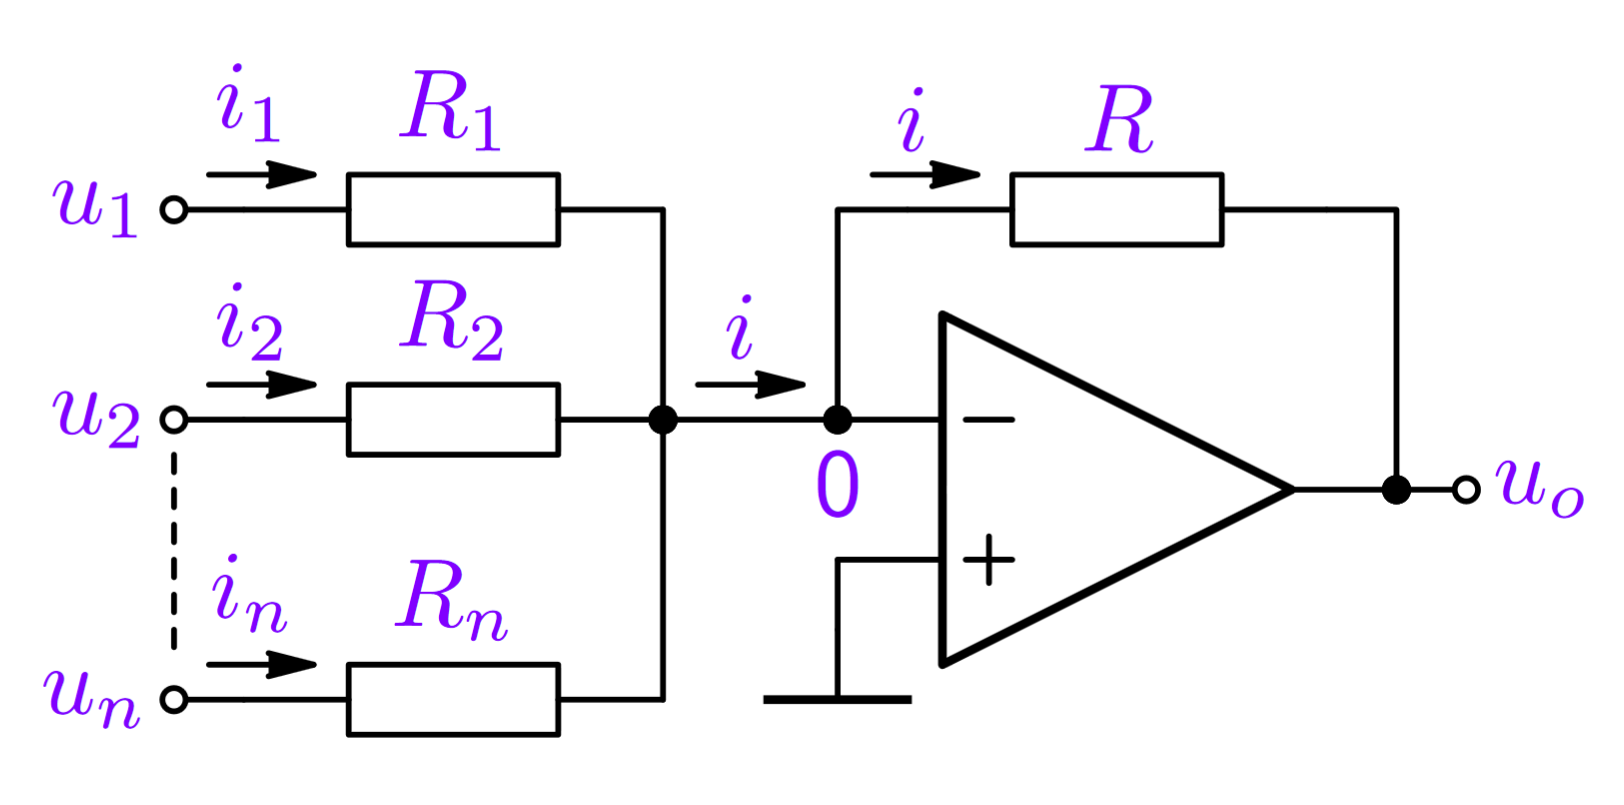
\includegraphics[width=.5\textwidth]{invert-sumator.PNG}
    \caption{Zapojení invertujícího sumátoru (proudové sčítačky)}
    \label{sch:sumator}
\end{schema}

Mantra říká, že do vstupu operáku nic neteče. Také říká, že na vstupech bude stejné napětí. Jestliže každý vstup vyrobí proud o~velikosti $i_k = \frac{u_k}{R_k}$ pro $k\in (1..n)$, tak celkový proud tekoucí do uzlu bude:
\begin{equation*}
    i_\Sigma=\sum_{k=1}^n i_k.
\end{equation*}
Stejný proud ale musí také někudy odtéct a~odteče jen a~pouze rezistorem R. Aby mohl takový proud odtéct, musí operační zesilovač stáhnout svůj výstup do záporna. A~jak moc do záporna?
\begin{equation}
    u_o = -u_R = -i_\Sigma R = -R \sum_{k=1}^n i_k = -R \sum_{k=1}^n \frac{u_k}{R_k}
\end{equation}

V motivaci bylo zmíněno, že se signály neovlivňují. Dokud je schopen OZ držet výše zmíněnou \textbf{virtuální zem}, každý vstup si bude myslet, že je jeho odpovídající rezistor $R_k$ skutečně připojen na zem resp. na fixní potenciál 0~V. Ačkoliv ho jen OZ bullshituje, protože koriguje výstup tak, aby na tomto sčítacím bodě bylo 0~V.

\textbf{A proč to taky umět?}\\
Protože tohle bylo ve zkoušce. Na první pohled divoký obvod je ve výsledku pouze jen nejjednodušší zapojení invertujícího sumátoru.
\begin{schema}
    \centering
    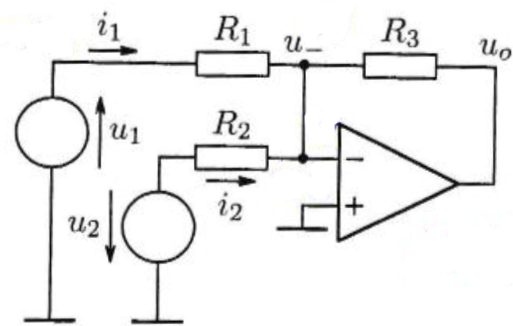
\includegraphics[width=.3\textwidth]{proudova_scitacka.PNG}
    \caption{Úloha z testu za 14 bodů}
\end{schema}






%10
\section{Nakreslete rozdílový zesilovač s~OZ a~odvoďte vztah pro výstupní napětí v~případě ideálního OZ. Definujte rozdílovou a~souhlasnou složku vstupního signálu a~odvoďte podmínku, pro kterou je souhlasná složka zesílení nulová. Co udává parametr CMMR?}
\href[pdfnewwindow=true]{http://hippo.feld.cvut.cz/vyuka/soubory/ElektronickeObvody.pdf#section.11.9}{\textit{Odkaz na odpovídající kapitolu v Hospodkových skriptách}}

\subsection*{Schéma, odvození vztahu}
\textbf{Motivace}: rozdílový zesilovač je supr čupr věc, která bere v~pozaz pouze rozdíl signálů. Pokud někam vedete signál dvěma vodiči a~nedejbože by se vám na nich naindukoval nějaký bordel, tak to je rozdílovému zesilovači úúúplně buřt. To proto, že naindukovaný bordel bude pro oba vodiče stejný a~to náš zesík nezajímá. Náš zesík zajímá pouze rozdíl signlálů a~ten zůstane nepolíben. Docela cool, co?

\begin{schema}[h!]
    \centering
    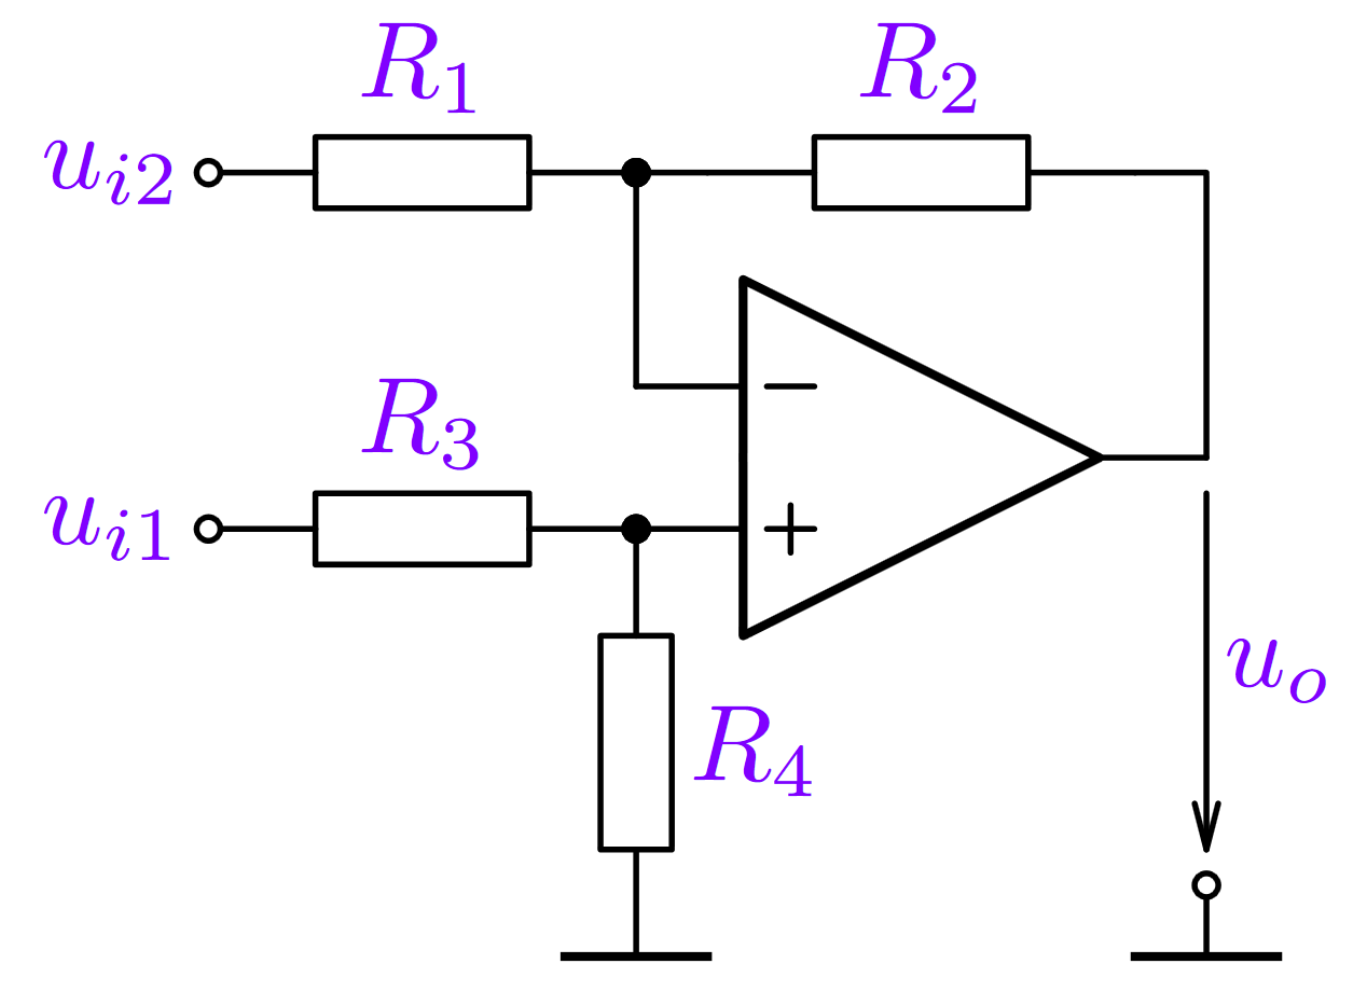
\includegraphics[width=.4\textwidth]{rozdilovy-zesilovac-oz.PNG}
    \caption{Rozdílový zesilovač s~OZ}
    \label{sch:rozdilovy:zesilovac}
\end{schema}

Při odvozování si pomůžeme superpozicí. Super pozice je třeba v~hospodě, ale superpozice nám pomůže teď stejně dobře. Vždy jeden vstup uzemníme a~počítáme ten neuzemněný:
\begin{schema}[h!]
    \centering
    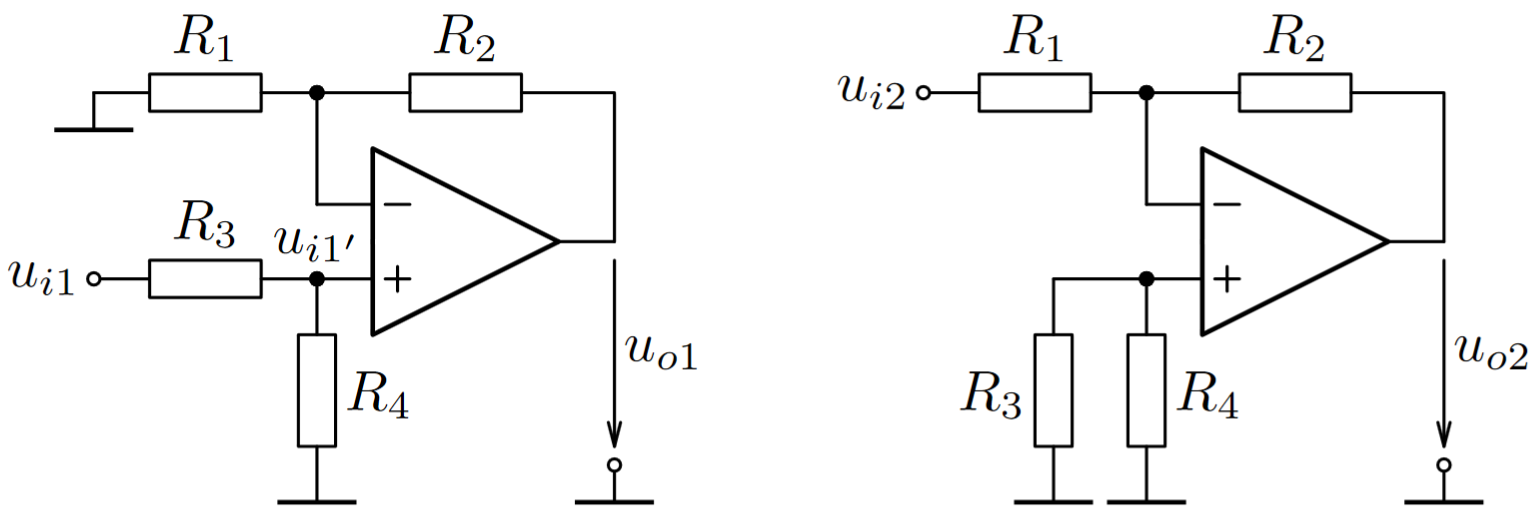
\includegraphics[height=.25\linewidth]{rozdilovy-zesilovac-oz-superpozice.PNG}
    \caption{Superpozice rozdílového zesilovače}
\end{schema}
\textbf{Vpravo} vidíme (sice vzůru nohama, ale přece) neinvertující zesilovač. Jen je zde navíc na vstupu do zesilovače další dělič napětí ($u_{i1}' = u_{i1}\frac{R_4}{R_3 + R_4}$). Tedy pro napětí $u_{o1}$ platí 
\begin{equation*}
    u_{o1} = u_{i1}'\left(1+\frac{R_2}{R_1}\right) = u_{i1}\frac{R_4}{R_3+R_4}\left(1+\frac{R_2}{R_1}\right)
\end{equation*}
\textbf{Vlevo} se nám zase narodil invertující zesilovač. Uzemněné rezistory $R_3, R_4$ nehrají roli a~pro zesílení resp. výstupní napětí plaví obyč vztah
\begin{equation*}
    u_{o2} = -u_{i2}\frac{R_2}{R_1}
\end{equation*}

Sečtením superponovaných napětí $u_{o1,2}$ dostaneme výsledný vztah pro $u_o$
\begin{equation}
    u_o = u_{i1}\frac{R_4}{R_3+R_4}\left(1+\frac{R_2}{R_1}\right)-u_{i2}\frac{R_2}{R_1}.
\end{equation}
Fuj, to je hnusnej vztah, kdo si to má pamatovat? Pokud si nebudeme znepříjemňovat život a~budeme se držet podmínky, že
\begin{equation*}
    \frac{R_4}{R_3} = \frac{R_2}{R_1},
\end{equation*}
tak pro výsledné napětí můžeme psát
\begin{equation}
    \underline{\underline{u_o = \frac{R_2}{R_1}(u_{i1}-u_{i2})}}.
\end{equation}
Vstupní odpor pro rozdílový signál bude
\begin{equation}
    \underline{\underline{R_{i_d} = R_1 + R_3}}.
\end{equation}


\subsection*{Souhlasná a~rozdílová složka + podmínka}
Souhlasná složka je definována jako
\begin{equation*}
    u_s = \frac{u_{i1} + u_{i2}}{2}.
\end{equation*}

Rozdílová poté jako
\begin{equation*}
    u_d = u_{i1} - u_{i2}.
\end{equation*}

\textbf{Podmínka}, aby byla souhlasná složka rušení nulová:
\begin{equation*}
    \frac{R_4}{R_3} = \frac{R_2}{R_1},
\end{equation*}

\begin{figure}[h!]
    \centering
    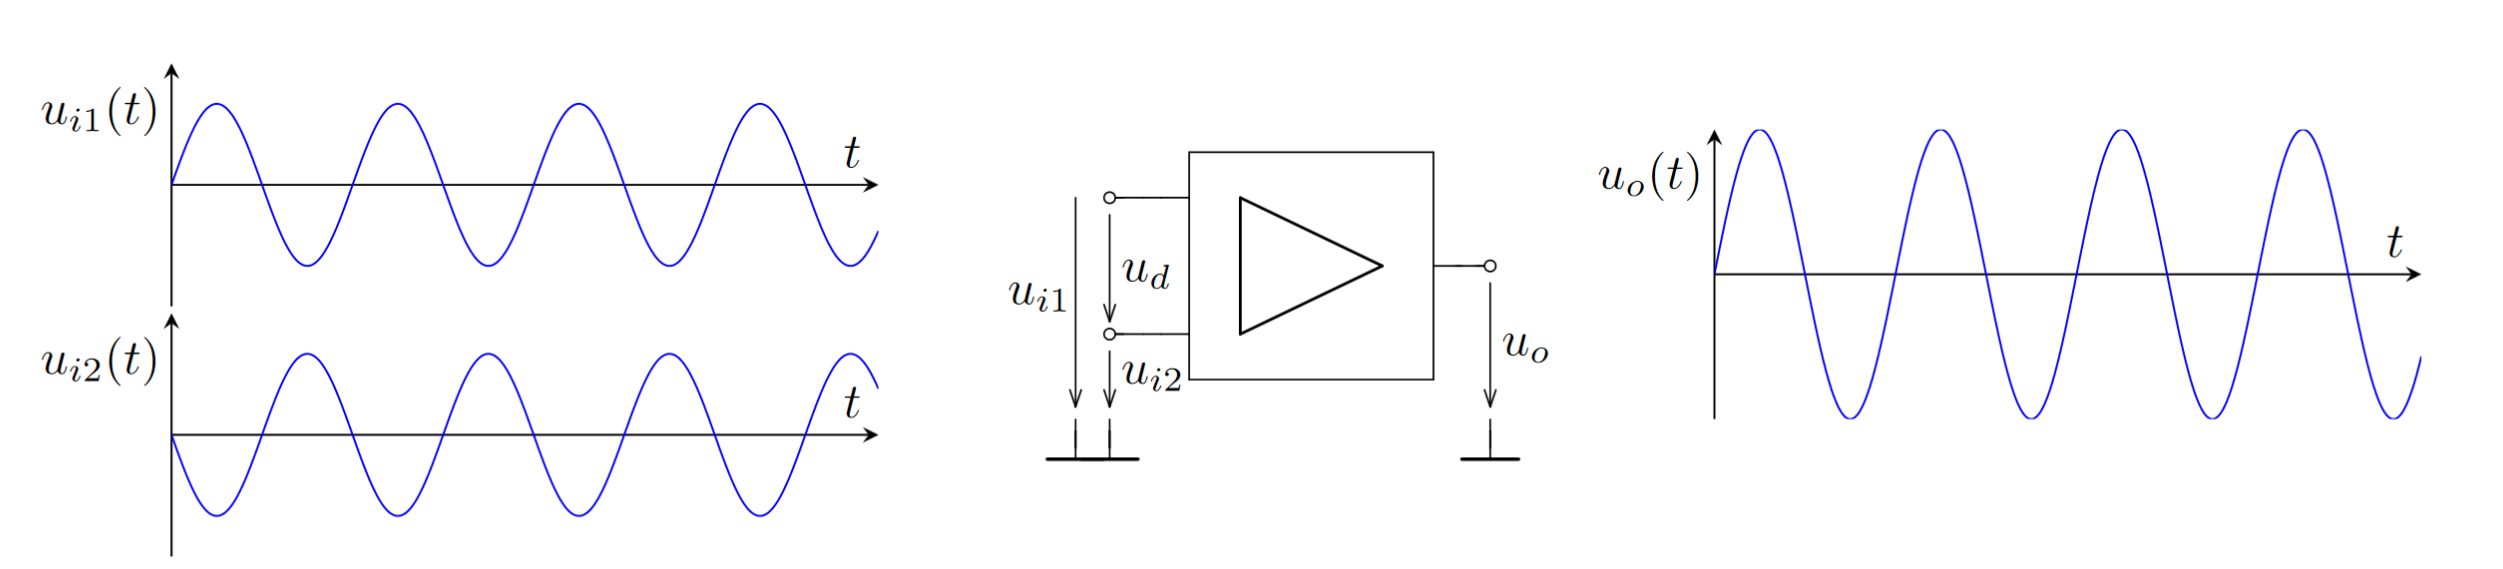
\includegraphics[width = \textwidth]{rozdilovy-zesilovac-signal.PNG}
    \caption{Oba vstupy vedou signál - s~opačnou polaritou. Tedy souhlasná složka $u_s$ bude nulová}
    \label{fig:rozdilovy:signal}
\end{figure}

\subsection*{Co je to CMMR}
\textbf{C}ommon \textbf{M}ode \textbf{R}ejection \textbf{R}atio.
\begin{equation}
    \text{CMMR} = \abs[\Big]{\frac{A_d}{A_s}}
\end{equation}
Sice by bylo naprosto epesní, kdyby zesilovač skutečně zesiloval pouze rozdíl, ale on bohužel zesiluje i~tu souhlasnou složku. Maximalizací CMMR se rozumí co největší poměr zesílení rozdílové složky vůči zesílení souhlasné složky.










%11
\section{Nakreslete zapojení převodníku proud-napětí s~OZ a~odvoďte převodní vztah pro případ ideálního OZ. Jaké jsou hlavní výhody a~nevýhody uvedené implementace.}
\href[pdfnewwindow=true]{http://hippo.feld.cvut.cz/vyuka/soubory/ElektronickeObvody.pdf#section.11.8}{\textit{Odkaz na odpovídající kapitolu v Hospodkových skriptách}}

\textbf{Motivace}: pokud posvítíme na fotodiodu, tak začne generovat proud úměrný intenzitě osvitu. Tento proud (řádově $\mu$A) ale potřebujeme převést na napětí, abychom ho mohli snímat např. mikrokontolérem. Proto využijeme převodník proud $\rightarrow$ napětí.

\begin{schema}
    \centering
    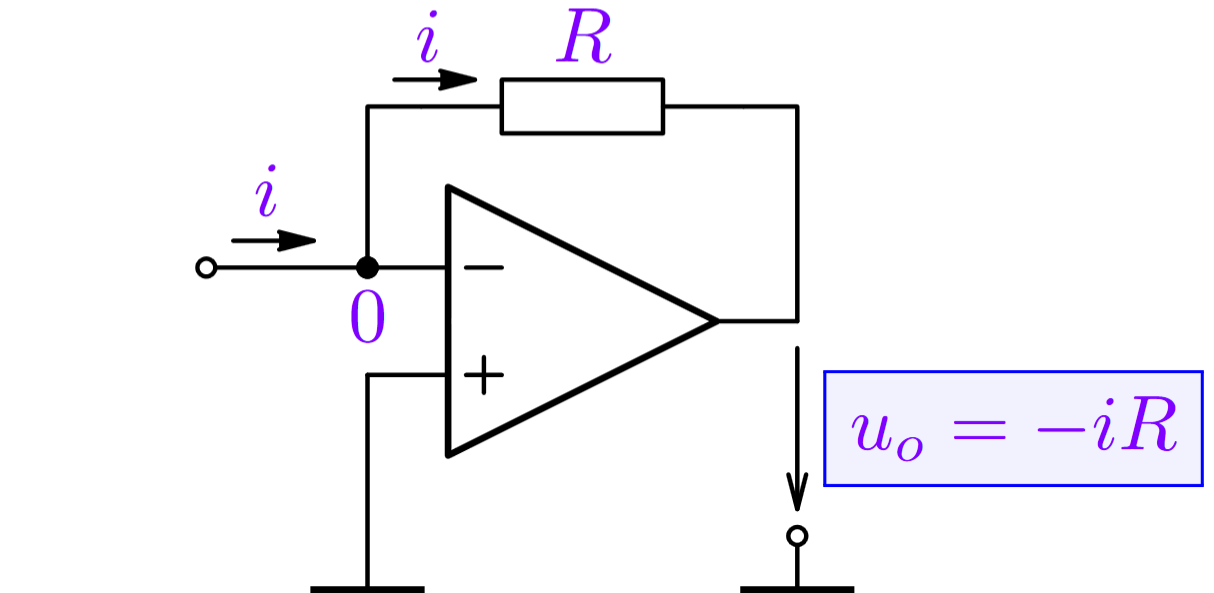
\includegraphics[width=.4\textwidth]{prevodnik-iu.PNG}
    \caption{Převodník proud - napětí}
    \label{sch:prevodnik:iu}
\end{schema}

Proud tekoucí do uzlu na invertujícím vstupu musí v~plné síle protéct dál do rezistoru $R$. Na vstupech operáku je stejné napětí a~jelikož je neinvertující vstup uzeměn, tak i~na invertujícím vstupu bude $0$~V. Proud $i$ tekoucí do převodníku poteče skrze rezistor, kde nastane úbytek napětí
\begin{equation}
    \underline{\underline{u_o = -i\,R}}.
\end{equation}

\textbf{Výhody}: s~dobrým operačním zesilovačem lze dosáhnout veliké přesnosti\footnote{Snažíme se minimalizovat proud, který poteče do vstupu operačního zesilovače. V~datasheetu se tento parametr jmenuje input bias current a~u obyč operáků může mít řádově $\mu$A. U~spešl operáků se dostaneme až na jednotky fA. FEMPTOAMPÉRY!! Zde vyložene počítáte počet kuliček elektronů za sekundu.}\\
\textbf{Nevýhody}: stejný proud, který snímáme, musí být operační zesilovač schopen odebrat na výstupu (current sink) - omezený rozsah. Další nevýhoda zapojení ve schématu \ref{sch:prevodnik:iu} je to, že můžeme snímat pouze proud, který by jinak tekl do země. To proto, že na invertujícím vstupu je \textbf{virtuální zem}. Nemůžeme tedy např. snímat proud tekoucí do báze tranzistoru, jelikož náš obvod umí snímat pouze proudy, které mají téct do země.






%12
\section{Nakreslete zapojení ideálního a~ztrátového invertujícího integrátoru s~OZ. Odvoďte jejich přenos a~nakreslete modulové charakteristiky s~popisem významných hodnot uvedených v~odvození.}
\href[pdfnewwindow=true]{http://hippo.feld.cvut.cz/vyuka/soubory/ElektronickeObvody.pdf#section.11.10}{\textit{Odkaz na odpovídající kapitolu v Hospodkových skriptách}}

\label{chap:integrator}
\textbf{Motivace}: Mega cool shit, můžete integrovat signál a~nepotřebujete k~tomu ani matlab. Lze využít také např. pro převod z~obdélníkového signálu na trojúhelníkový. 

\begin{figure}[h!]
    \centering
    \begin{subfigure}{.49\textwidth}
        \centering
        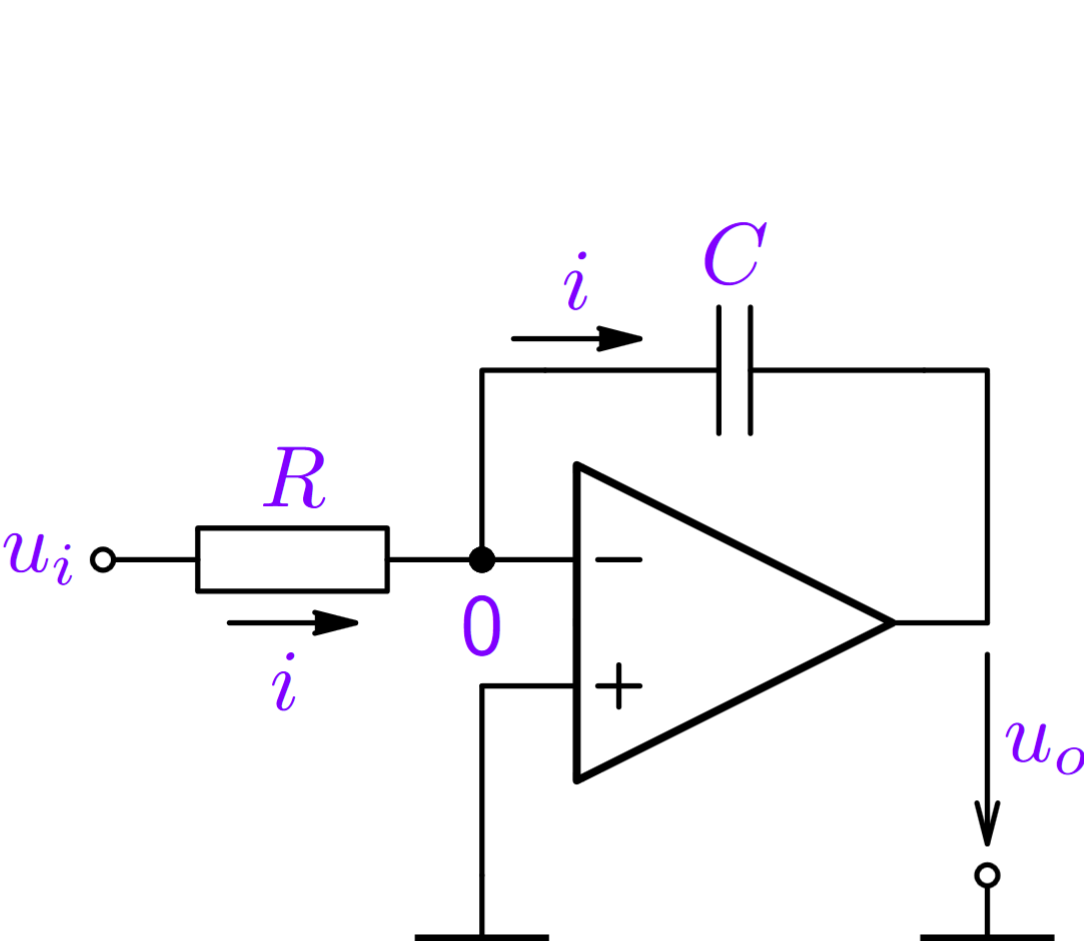
\includegraphics[height=.5\linewidth]{integrator-ideal.PNG}
        \caption{Ideální integrátor}
        \label{sch:integrator:ideal}
    \end{subfigure}
    \begin{subfigure}{.49\textwidth}
        \centering
        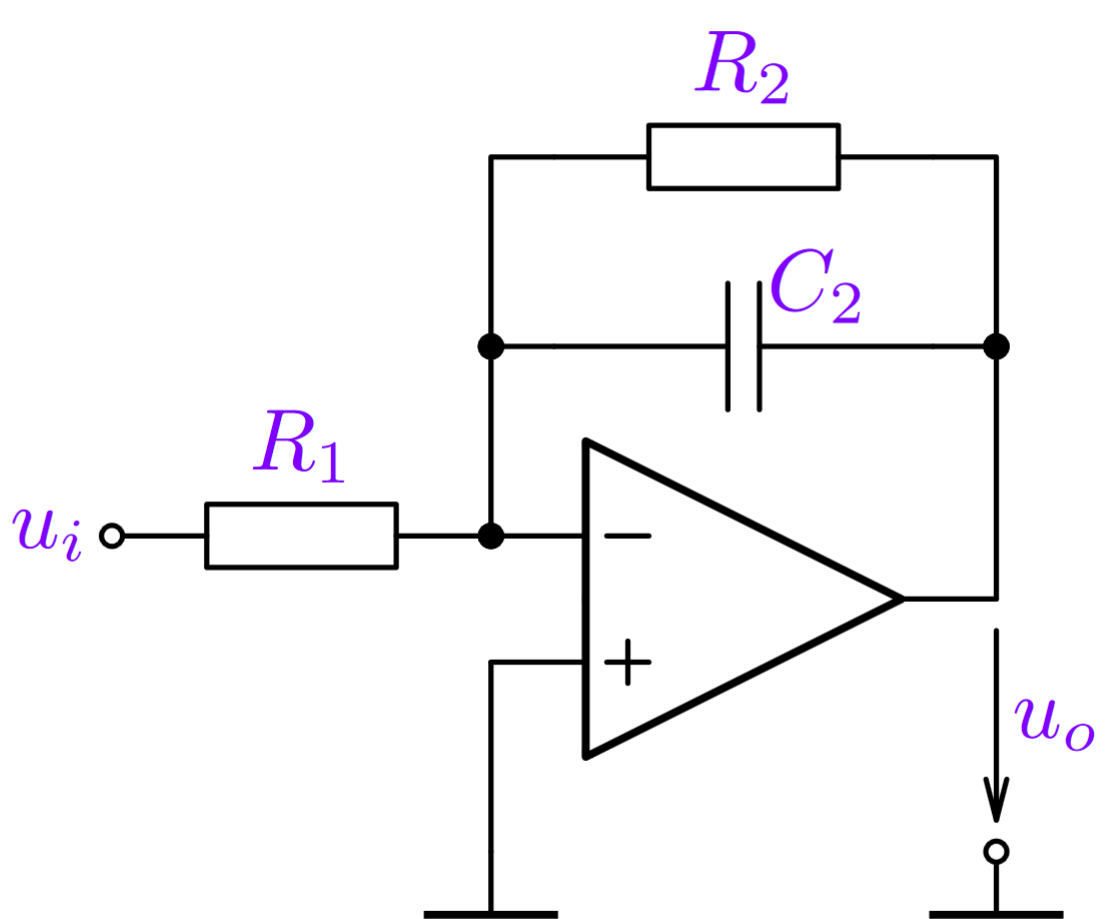
\includegraphics[height=.5\linewidth]{integrator-real.PNG}
        \caption{Ztrátový integrátor}
        \label{sch:integrator:ztatovy}
    \end{subfigure}
\end{figure}

\subsection*{Ideální integrátor}
Pro proud tekoucí kondenzátorem platí
\begin{equation*}
    i(t) = C\frac{\text{d}u}{\text{d}t}.
\end{equation*}
Z toho si lze vyjádřit napětí jako
\begin{equation*}
    u(t) = u_c(0) + \frac{1}{C}\int_0^t i(x)\text{d}x =//i=\frac{u_i}{R}//= u_c(0) + \frac{1}{RC}\int_0^t u(x)\text{d}x.
\end{equation*}

Naše zapojení vypadá skoro jako invertující zesilovač, jen místo jednoho rezistoru je kondenzátor. U~popisu invertujícího zesilovače jsme dělali jistou myšlenkovou gymnastiku, abychom vysvětlil, proč bude na výstupu \textbf{záporné} napětí. (napětí na kondenzátoru měříme ve směru proudu tedy od invertujícího vstupu (0~V) vůči výstupu operáku). Naopak napětí na výstupu měříme od onoho výstupu vůči zemi - tedy opačný směr a~opačné znaménko.

\begin{equation*}
    u_o(t) = - u_c(0) - \frac{1}{RC}\int_0^t u(x)\text{d}x.
\end{equation*}

\textbf{Přenos systému je poté}
\begin{equation}
    H(s) = \frac{U_o(s)}{U_i(s)} = -\frac{1}{s\tau}~,~~~~\tau = RC
\end{equation}
\begin{graf}
    \centering
    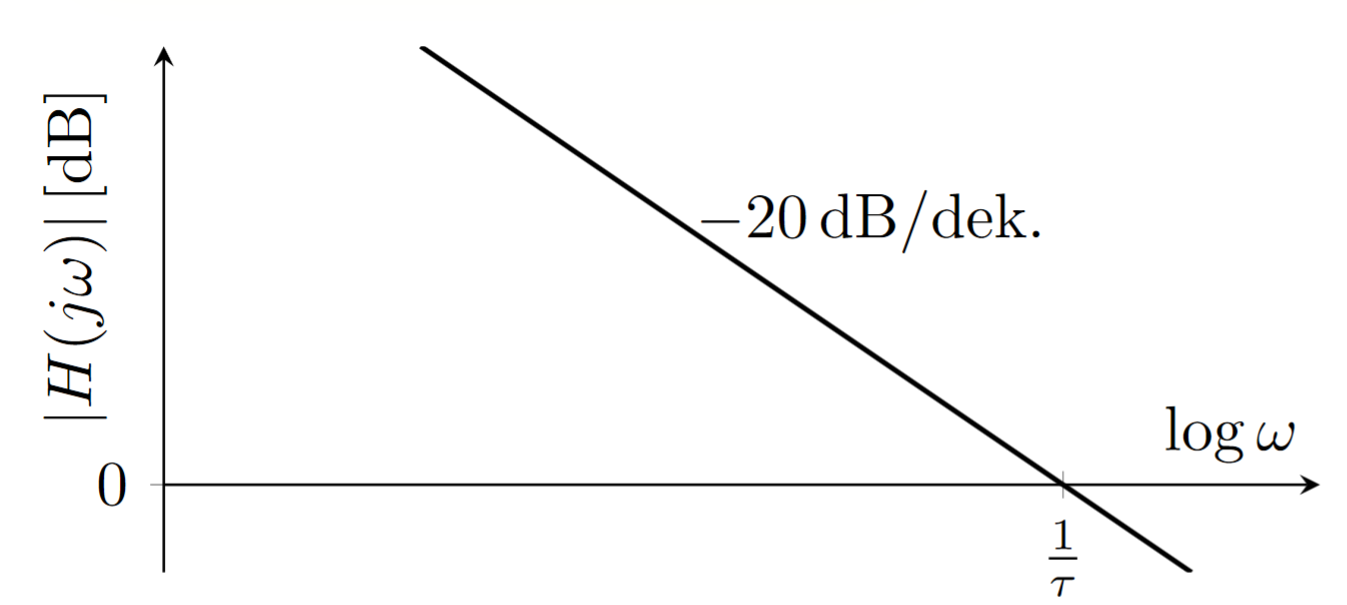
\includegraphics[width=.7\textwidth]{integrator-ideal-prenos.PNG}
    \caption{Přenos ideálního integrátoru}
\end{graf}

\subsection*{Ztrátový integrátor}
Kondenzátor by se nám ale při integraci mohl nabíjet do nekonečna. Abychom zabránili tomu, že narazíme na limit napájecího napětí operačního zesilovače, přidáme paralelně s~kondenzátorem ještě rezistor. Ten zajistí, že maximální napětí na výstupu bude omezeno \uv{jako kdyby to byl jen invertující zesilovač}.
\begin{equation}
    H(s) = -\frac{Z_2}{R_1} = \frac{\frac{R_2}{1+sC_2R_2}}{R_1} = -\frac{R_2}{R_1}\frac{1}{1-sC_2R_2} = \frac{H_0}{1+s\tau},
\end{equation}
kde $H_0 = -\frac{R_2}{R_1},~~~\tau_2 = C_2 R_2,~~~\omega_0 = \frac{1}{\tau_2}$
\begin{graf}
    \centering
    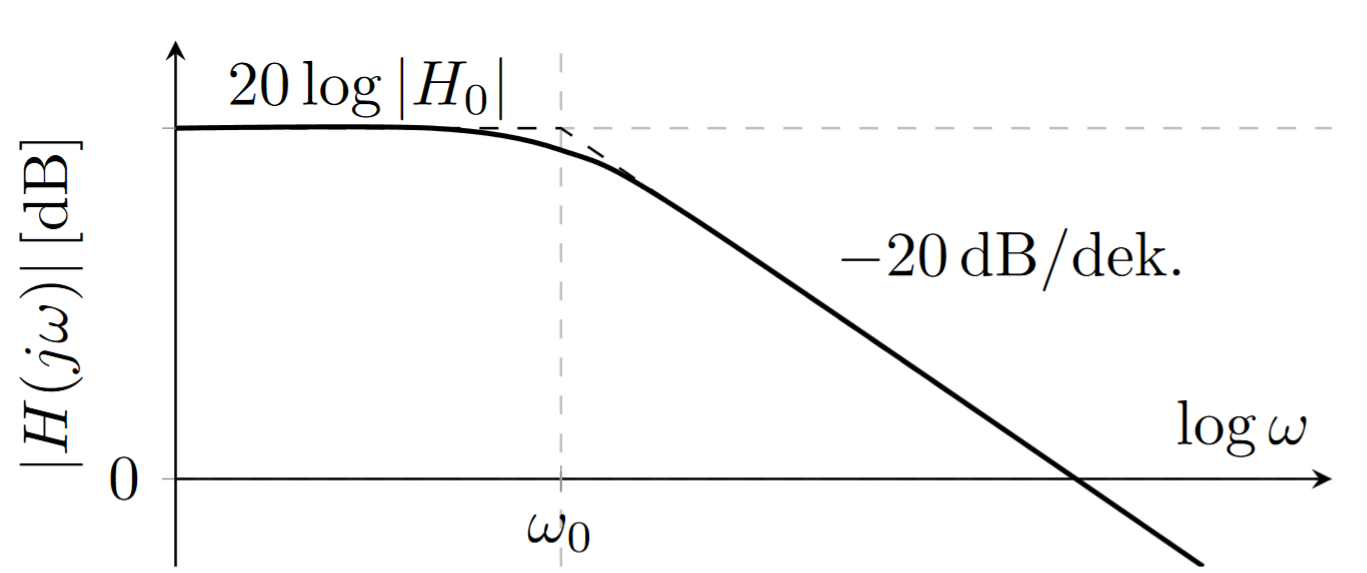
\includegraphics[width=.7\textwidth]{integrator-real-prenos.PNG}
    \caption{Přenos ztrátového integrátoru}
\end{graf}

\textit{Pozn:} chová se to jako lowpass, což není náhoda u~systémů, co integrují vstupní signál. Pokud půjdeme s~frekvencí nízko, tak se kondenzátor bude chovat jako rozpojené svorky a~tedy se uplatní pouze rezistory tvořící invertující zesilovač. Naopak při vysokých frekvencích se bude kondenzátor chovat jako zkrat a~paralelní kombinace $R_2||C_2$ bude mít minimální odpor. Zesílení zesilovače je dáno jako $A_u = -\frac{R_2||C_2}{R_1}$. Jestliže se pro vysoké frce snižuje impedance paralelní kombinace, bude se pro vyšší frce snižovat také zesílení. Cool init?






%13
\section{Nakreslete typické modulové charakteristiky neinvertujícího zesilovače s~OZ pro zesílení $A_u = 1, 10 \text{ a~} 100$, pokud je tranzitní kmitočet OZ $f_t=1$ MHz}
\href[pdfnewwindow=true]{http://hippo.feld.cvut.cz/vyuka/soubory/zv.pdf#page.29}{\textit{Odkaz na odpovídající kapitolu v Hospodkových skriptách}}

Modulová charakteristika resp. přenos v~závisloti na frekvenci je zobrazen v~grafu \ref{graph:modulova:charakteristika}. Zesílení jsou v~rámečku napsaná a~tranzientní kmitočet $f_t$ je tam, kde to jde prostě všechno do kopru. V~ten moment přestane zesilovač zesilovat.
\begin{graf}
    \centering
    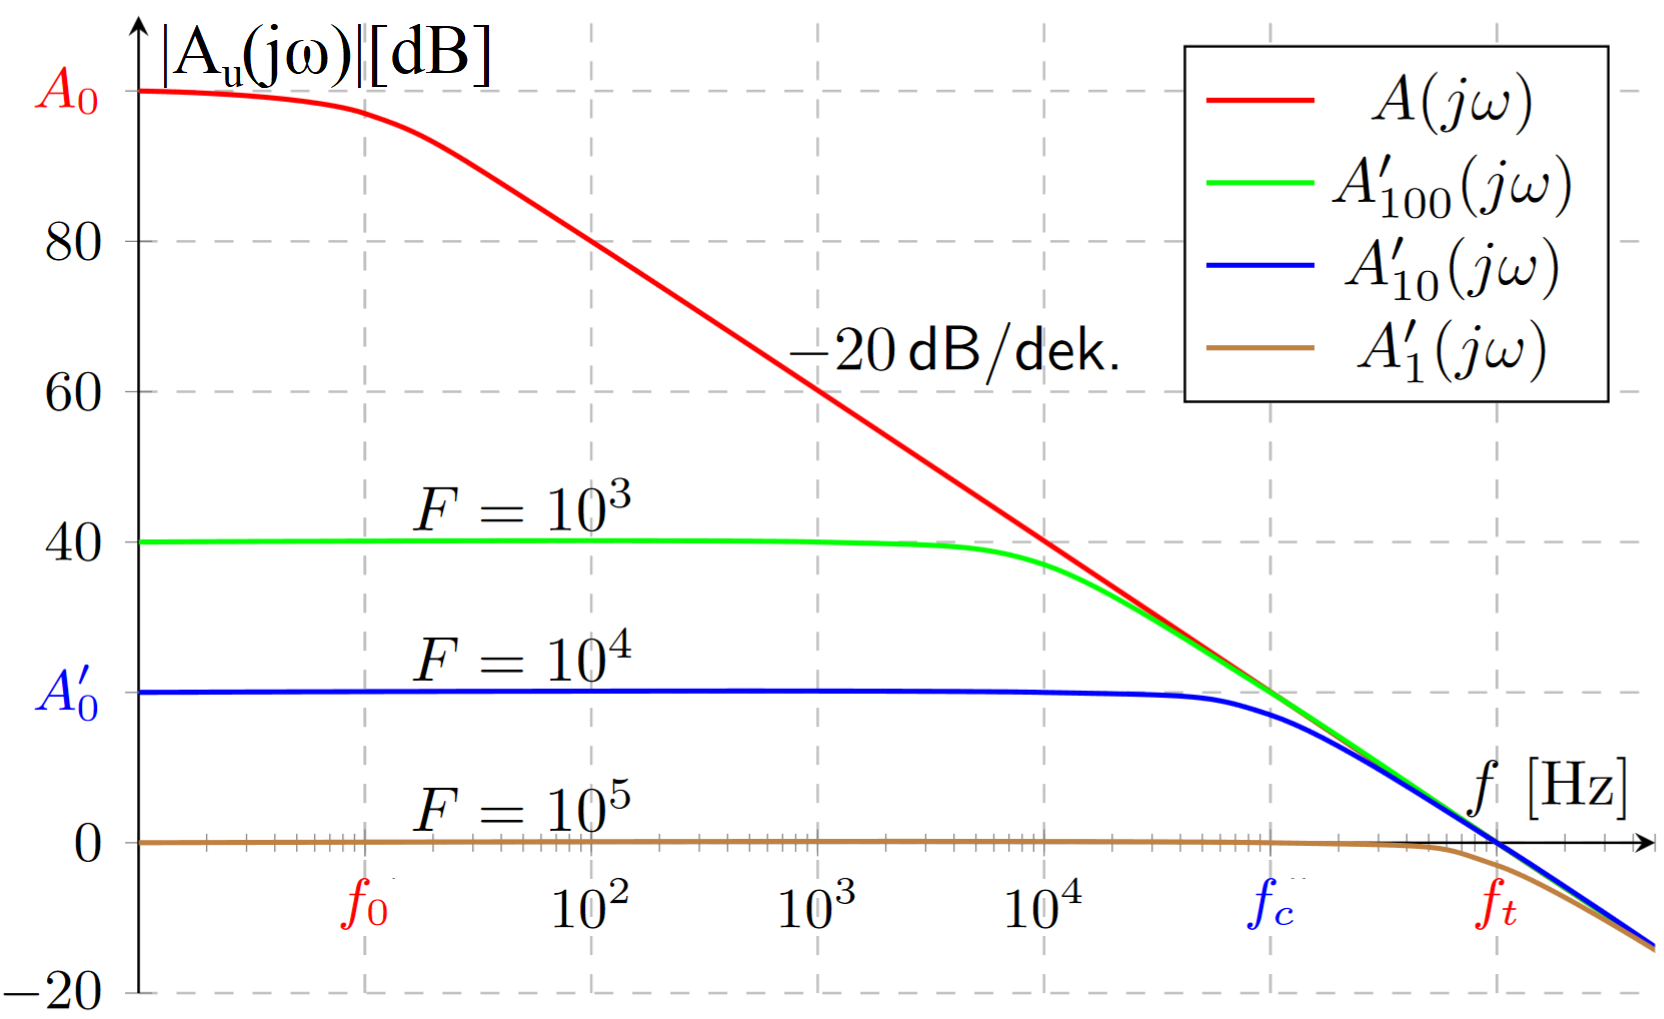
\includegraphics[width=.7\textwidth]{opamp-modulove_charakteristiky.PNG}
    \caption{Modulové charakteristiky operačního zesilovače}
    \label{graph:modulova:charakteristika}
\end{graf}

Červená křivka $A$ je open loop zesílení bez zavedené zpětné vazby. Další průběhy jsou již pro OZ se zpětnou vazbou.








%14
\section{Nakreslete zapojení jednocestného usměrňovače s~OZ, popište jeho činnost a~nakreslete časové průběhy na jednotlivých výstupech, včetně výstupu vlastního OZ při harmonickém buzení.}
\href[pdfnewwindow=true]{http://hippo.feld.cvut.cz/vyuka/soubory/ElektronickeObvody.pdf#section.11.16}{\textit{Odkaz na odpovídající kapitolu v Hospodkových skriptách}}

\textbf{Motivace}: reálná dioda se začne otevírat až v~momentě, kdy úbytek napětí na ní je větší než cca $u_d = 0.6$~V. Proto je nemožné usměrňovat signály s~nižším napětím. Tento problém elegantně řeší právě usměrňovač s~OZ, který dokáže kompenzovat úbytek napětí na diodě.

\begin{figure}
    \centering
    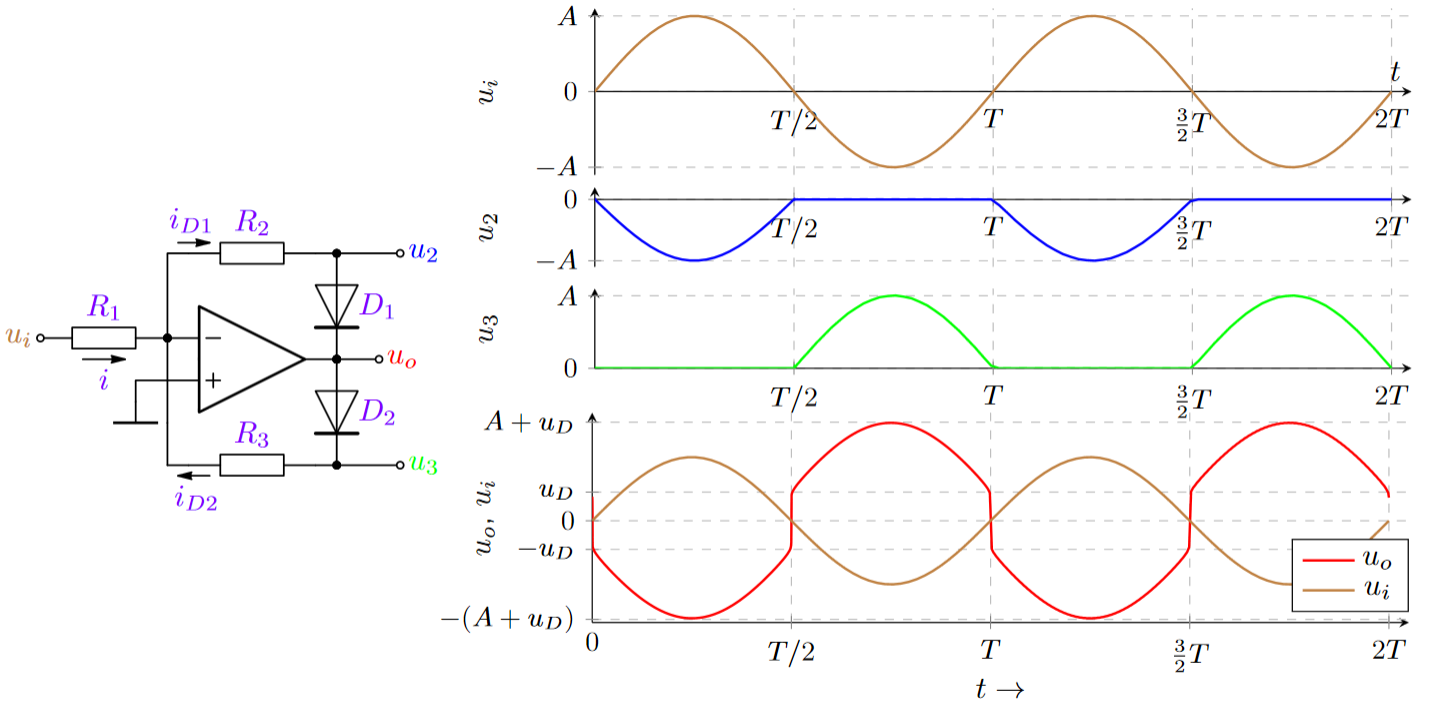
\includegraphics[width=\textwidth]{jednocestny-usmernovac.PNG}
    \caption{Jednocestný invertující usměrňovač}
    \label{fig:jednocestny:usmernovac}
\end{figure}
\begin{figure}
    \centering
    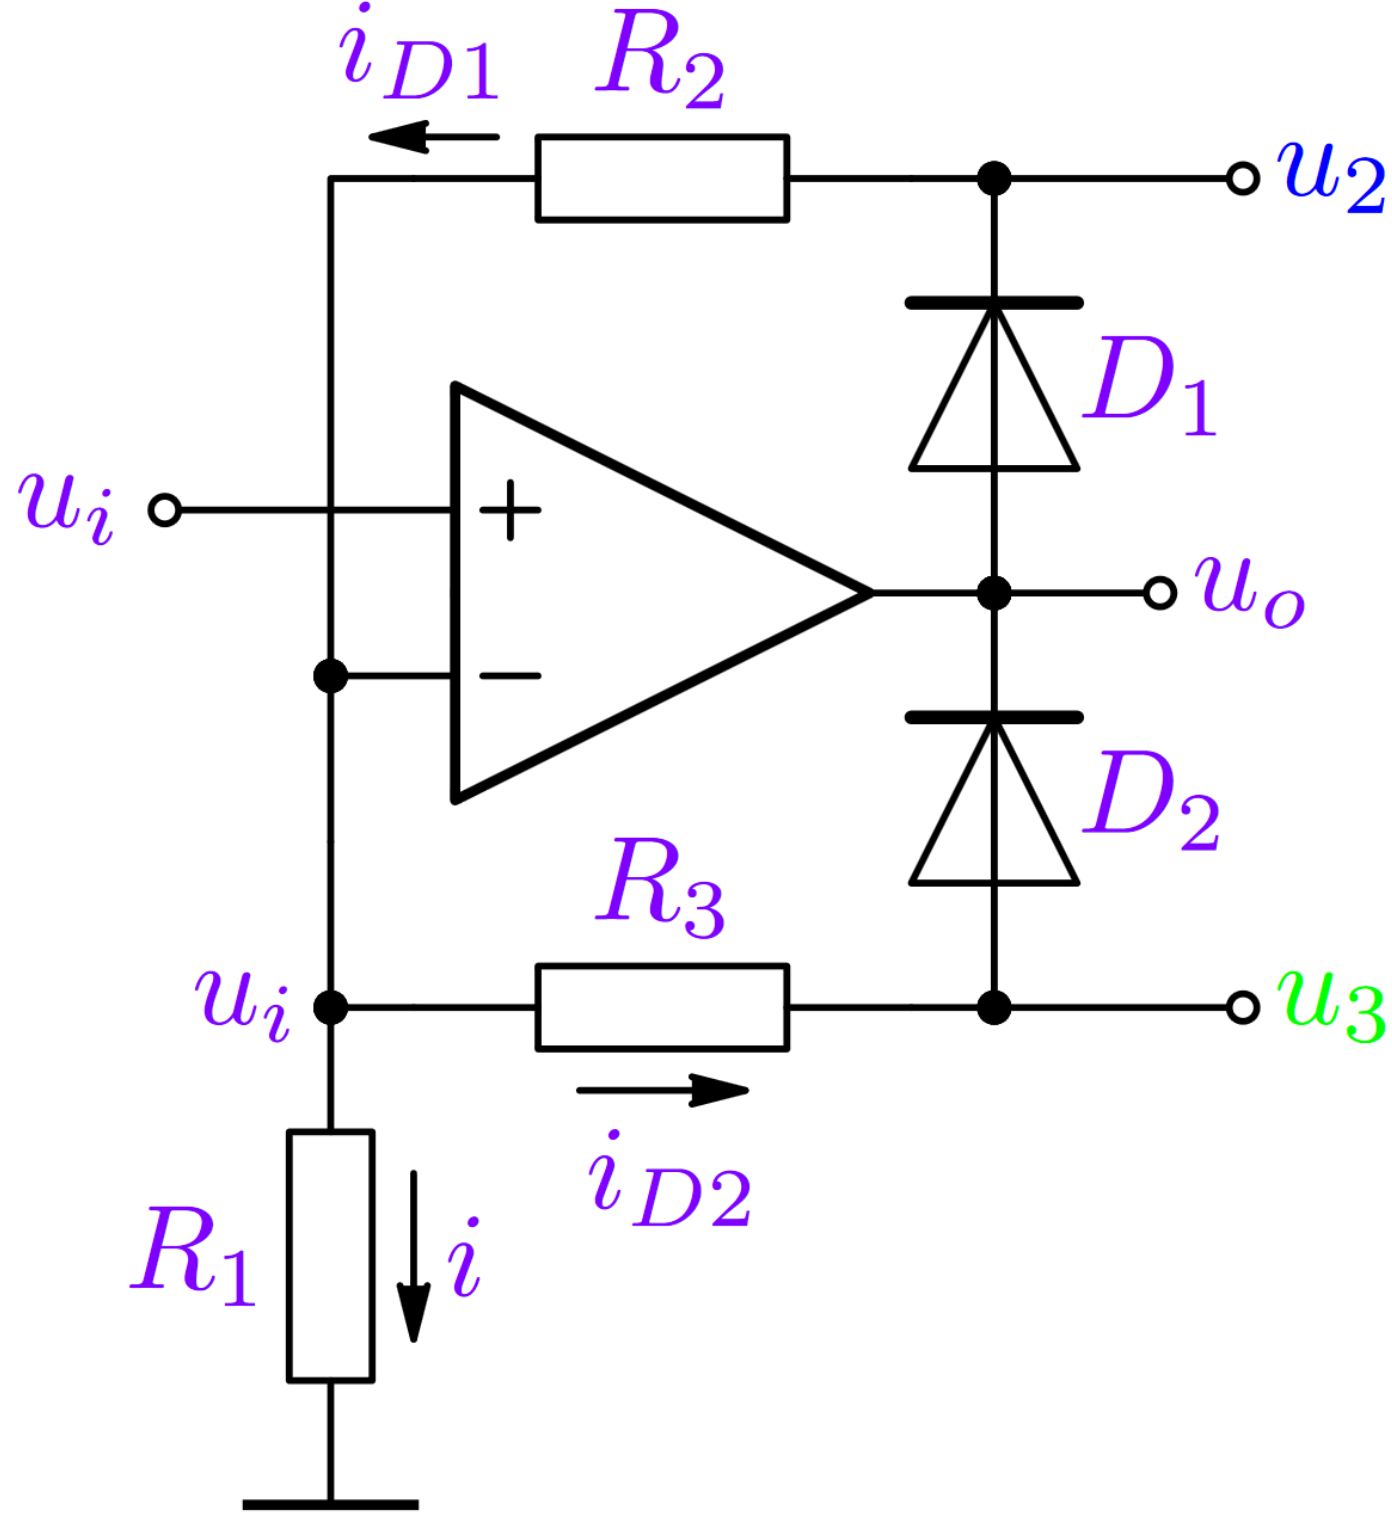
\includegraphics[width = .3\textwidth]{jednocestny-usmernovac-noninvert.PNG}
    \caption{Jednocestný neinvertující zesilovač}
    \label{fig:jendocestny:usmernovat:noninvert}
\end{figure}

Zapojení se chová jako klasický invertující zesilovač s~tím rozdílem, že ve zpětné vazbě je dioda, která ubírá cca $u_d = 0.6$~V. O~tuto hodnotu bude vždy výstup offsetnut. Pokud má operák zajistit na invertujícím vstupu 0~V, musí napětí na výstupu ještě \uv{přebít} úbytek napětí na diodě. Jak je vidět na dolním grafu z~obrázku \ref{fig:jednocestny:usmernovac}.








%15
\section{Nakreslete zapojení dvoucestného usměrňovače s~OZ, popište jeho činnost a~nakreslete časové průběhy na jednotlivých výstupech při harmonickém buzení.}
\href[pdfnewwindow=true]{http://hippo.feld.cvut.cz/vyuka/soubory/ElektronickeObvody.pdf#section.11.18}{\textit{Odkaz na odpovídající kapitolu v Hospodkových skriptách}}

\textbf{Motivace} stejná jako u~jednocestného, ale místo toho, aby se záporná složka ořízla a~poslala do kopru, tak je přivedena a~invertována. Viz dále.

\begin{schema}[h!]
    \centering
    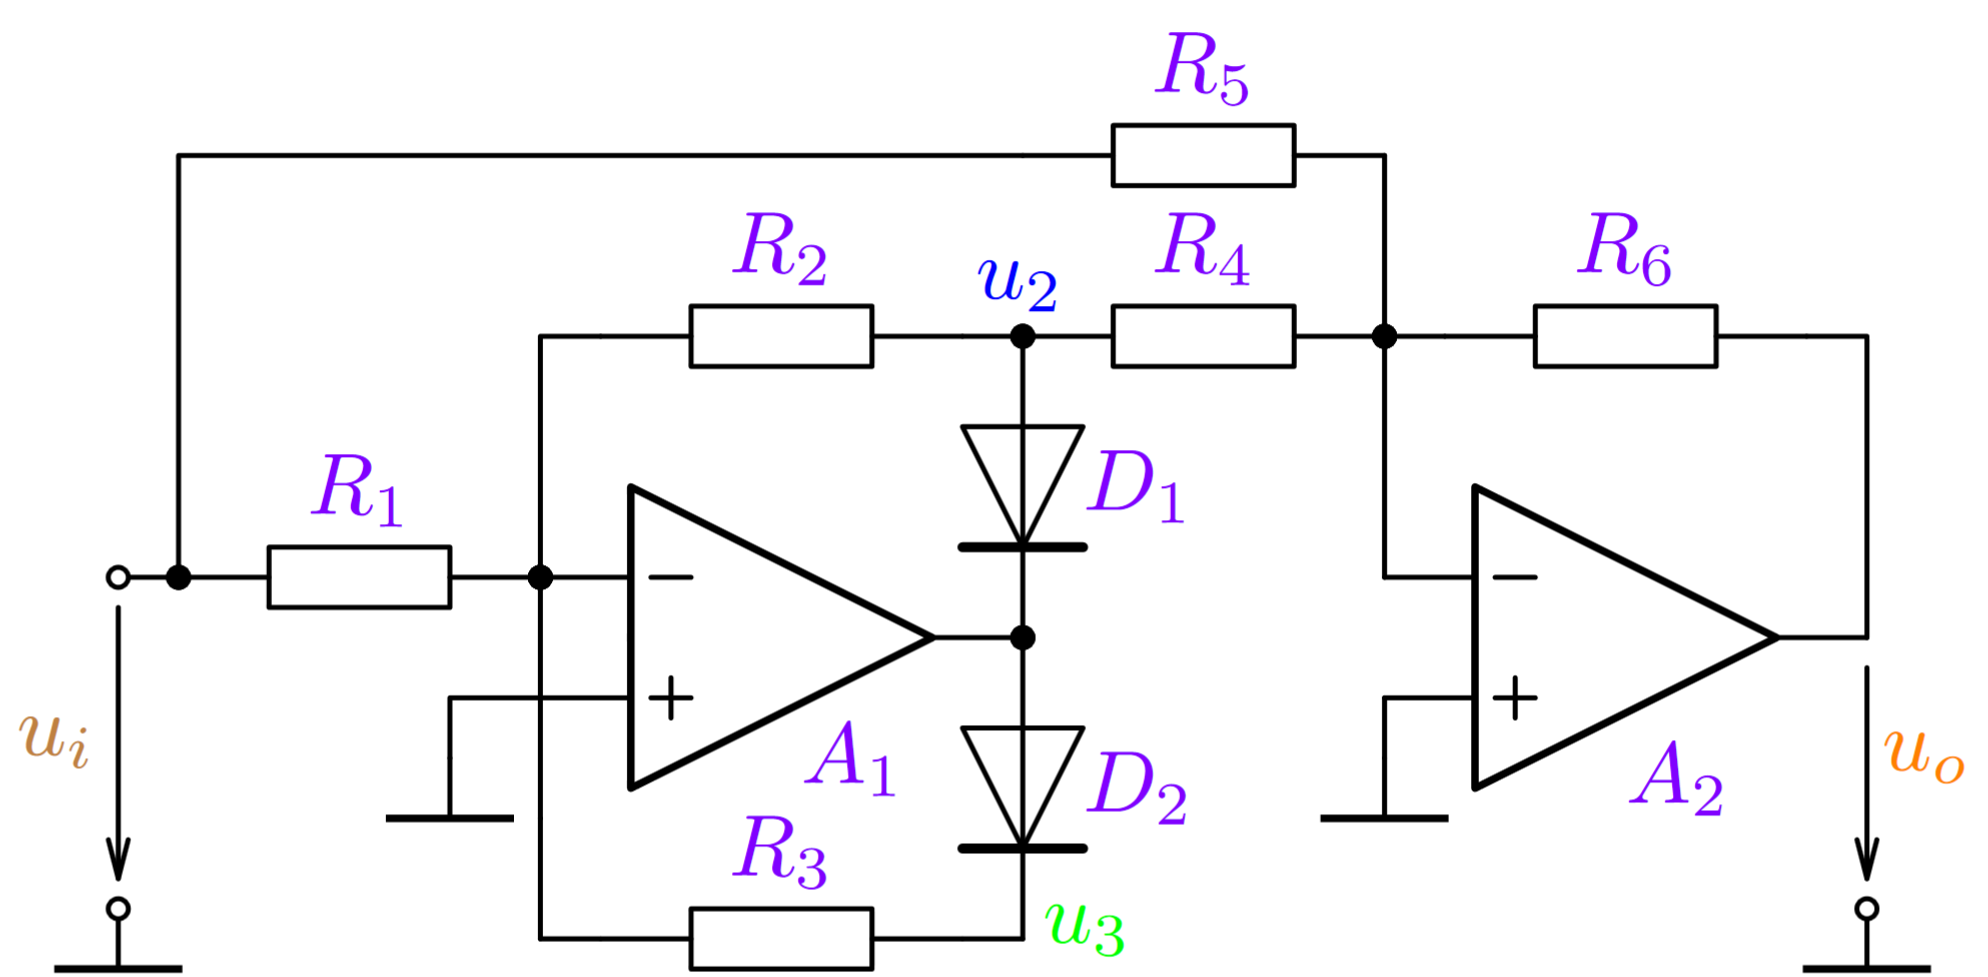
\includegraphics[width=.6\textwidth]{dvoucestny_usmernovac.PNG}
    \caption{Dvoucestný usměrňovač s~proudovou sčítačkou}
    \label{sch:dvoucestny:usm}
\end{schema}

\begin{graf}[h!]
    \centering
    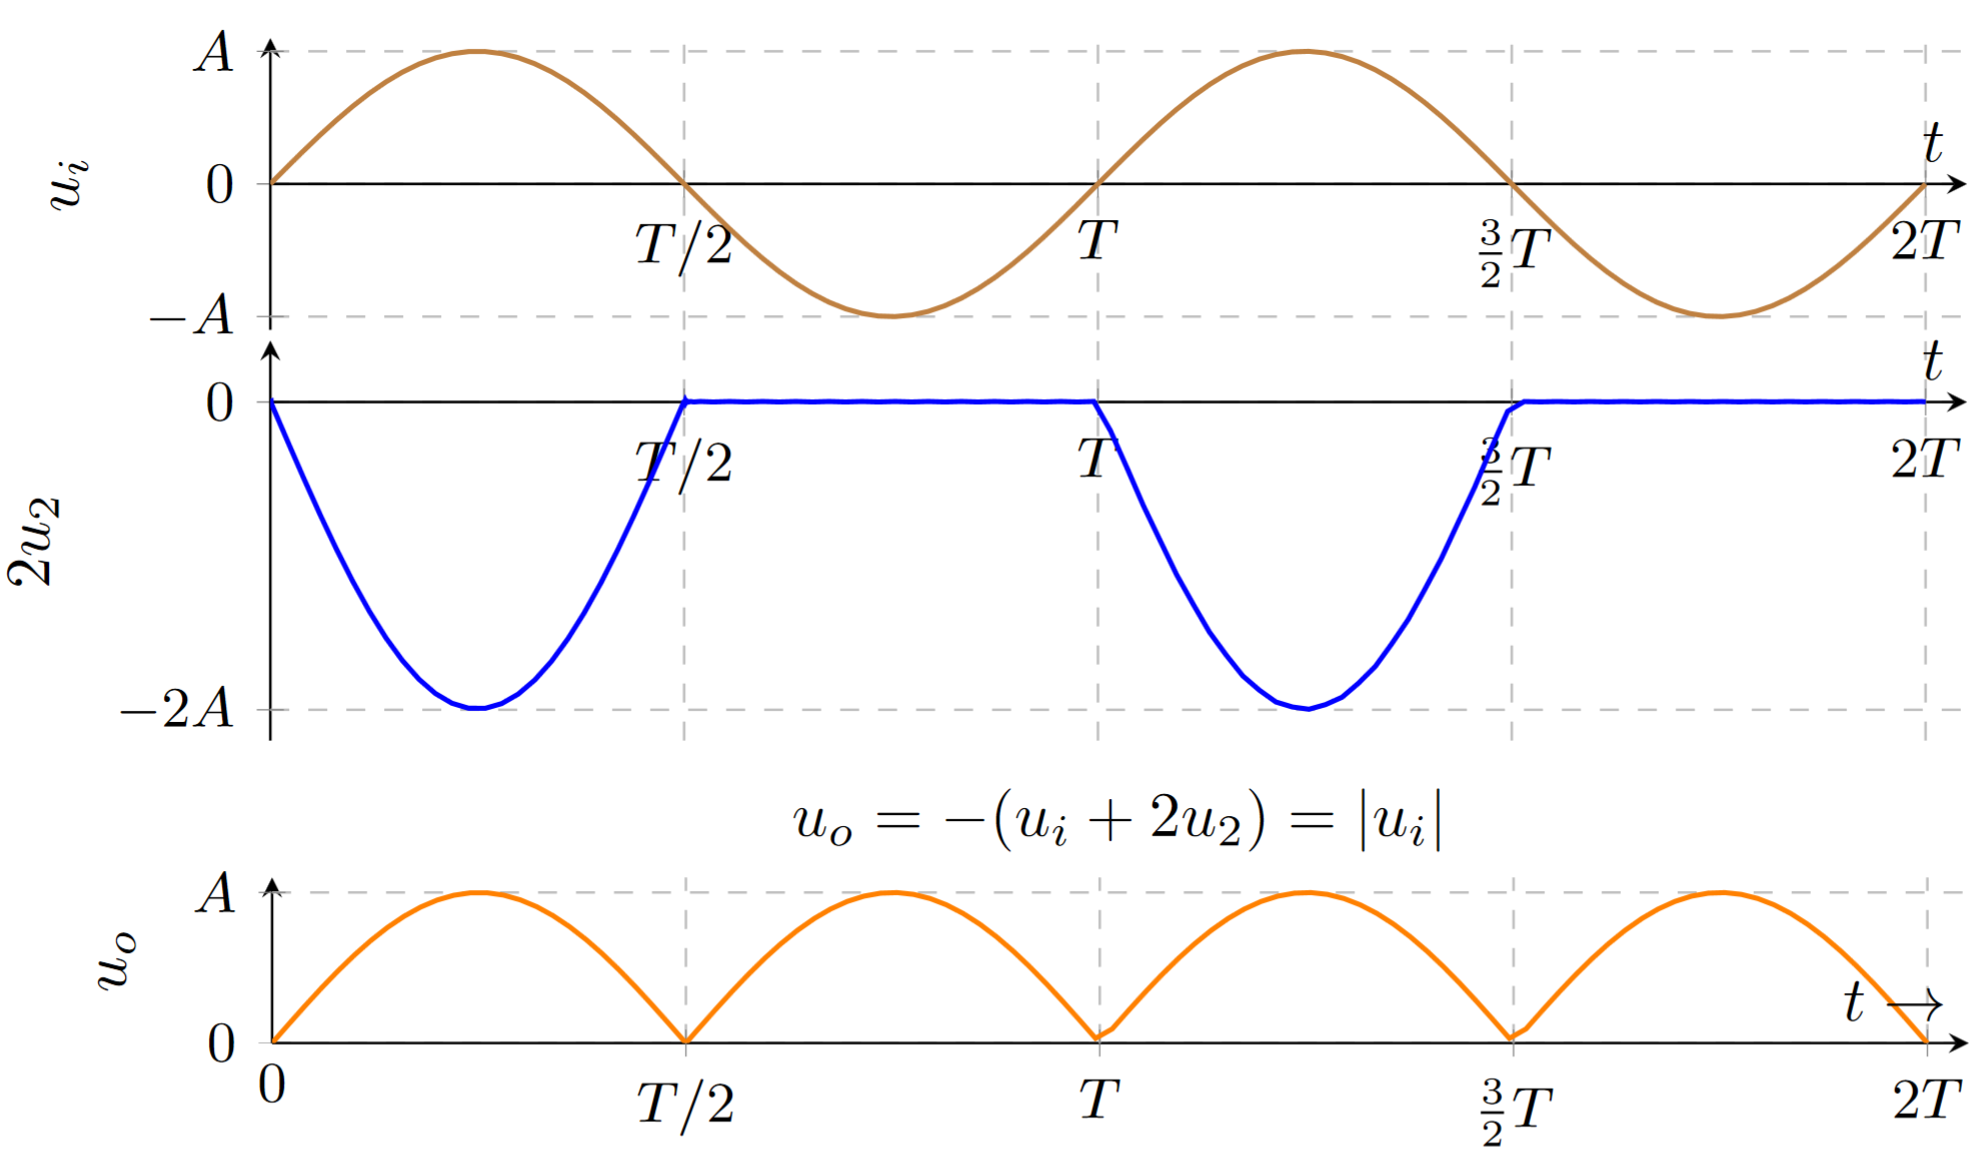
\includegraphics[width=.7\textwidth]{dvoucestny_usmernovac-prubeh.PNG}
    \caption{Časové průběhy v~obvodu s~dvoucestným usměrňovačem}
    \label{graf:dvoucestny:ums}
\end{graf}

Schéma \ref{sch:dvoucestny:usm} je tvořeno dvěma bloky. Jednocestným usměrňovačem a~sčítačkou napětí (proudu). Jak bylo zmíněno v~kapitole od OZ, tato sčítačka obrací polaritu. Výstup jednocestného usměrňovače je v~bodě $u_2$. Odtud jde signál skrze $R_4$ do sčítačky. Origo signál jde do sčítačky skrze $R_5$. Rezistory $R_4$ a~$R_5$ slouží k~váhování vstupních signálů jdoucích do sčítačky a~pokud chceme docílit modrého průběhu ve grafu \ref{graf:dvoucestny:ums}, musí platit, že $R_5 = 2R_4$. Díky tomu bude výstup jednocestného usměrňovače dvakrát větší zesílení oproti signálu jdoucí do $R_5$.

Z grafu je poté patrné, že sčítačka takto sečte vstupní signály (hnědý a~modrý) a~vznikne signál oranžový.





%16
\section{Nakreslete zapojení neinvertujícího a~invertujícího komparátoru s~hysterezí, uveďte jeho převodní charakteristiku a~odvoďte vztahy pro překlápěcí úrovně.}
\label{chap:komp}
\href[pdfnewwindow=true]{http://hippo.feld.cvut.cz/vyuka/soubory/ElektronickeObvody.pdf#section.11.19}{\textit{Odkaz na odpovídající kapitolu v Hospodkových skriptách}}

\textbf{Motivace}: pokud máme např. pomalé průběhy, nebo zašumělný signál, může nastat situace, kdy komparátor sice detekuje dostatečně vysoké napětí a~na výstup dá odpovídající hodnotu, ale šum může způsobit krátké oscilace, jak se zobrazeno na grafu \ref{graf:komp:nonhys}.
\begin{graf}
    \centering
    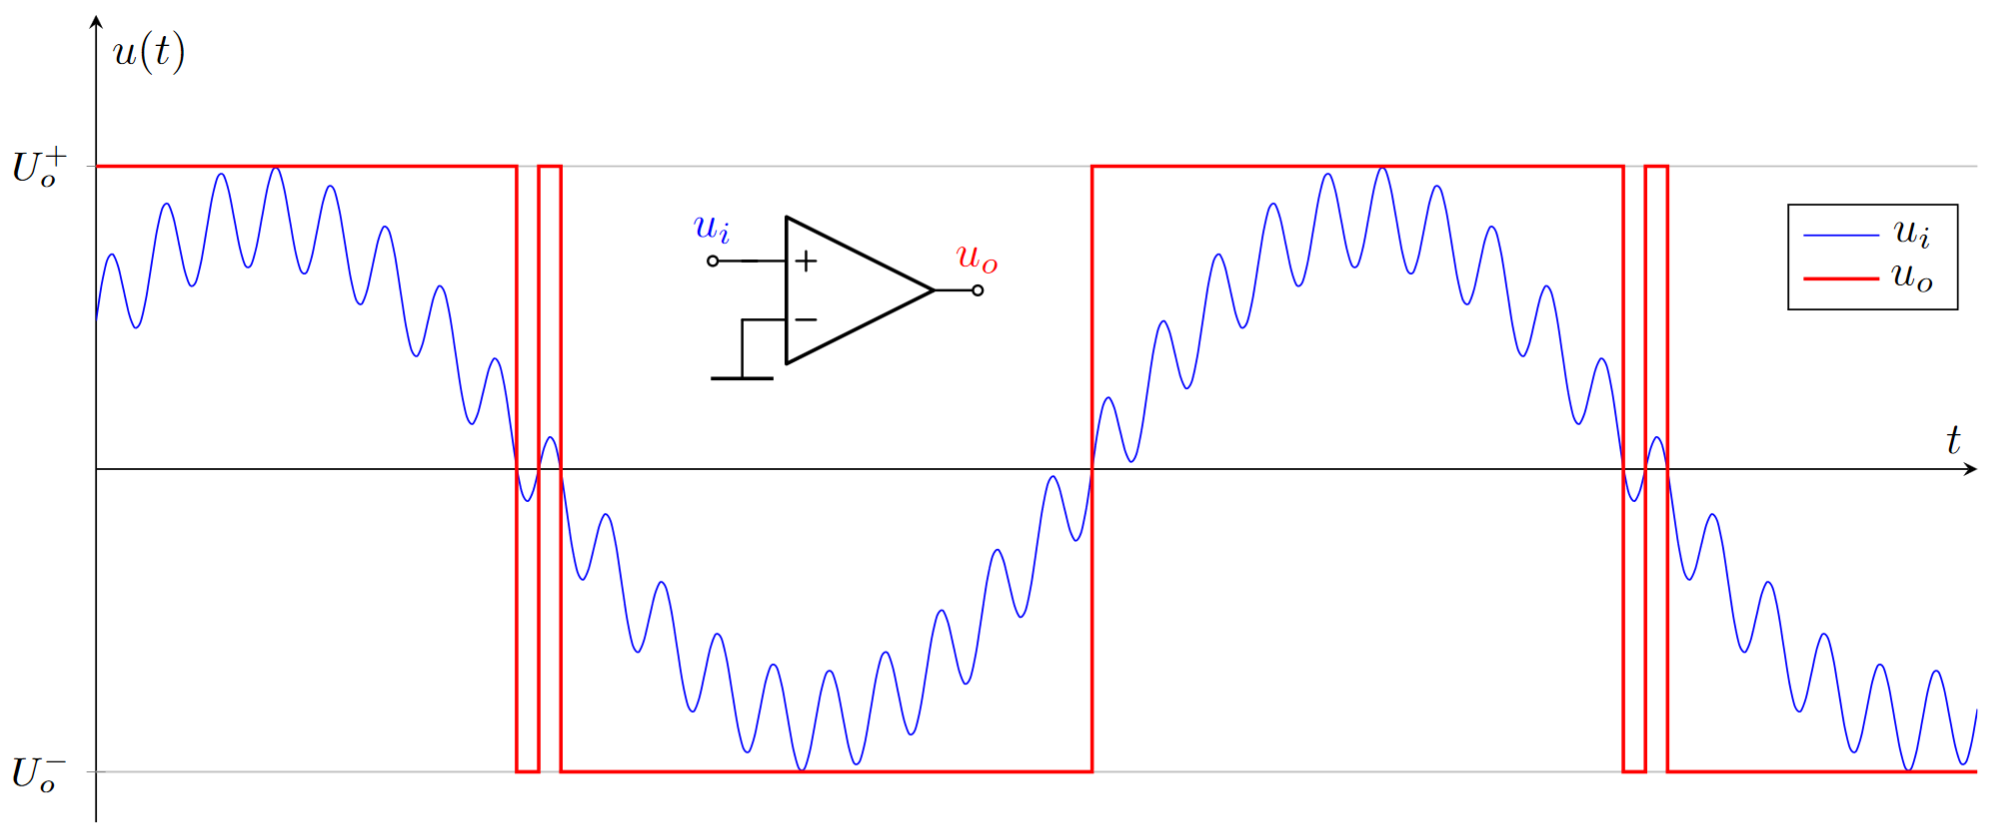
\includegraphics[width=.7\textwidth]{komparator-nehyst-graf.PNG}
    \caption{Výstup komparátoru bez hystereze}
    \label{graf:komp:nonhys}
\end{graf}

Pokud zavedeme hysterezi, bude výstup komparátoru vypadat následovně:
\begin{graf}
    \centering
    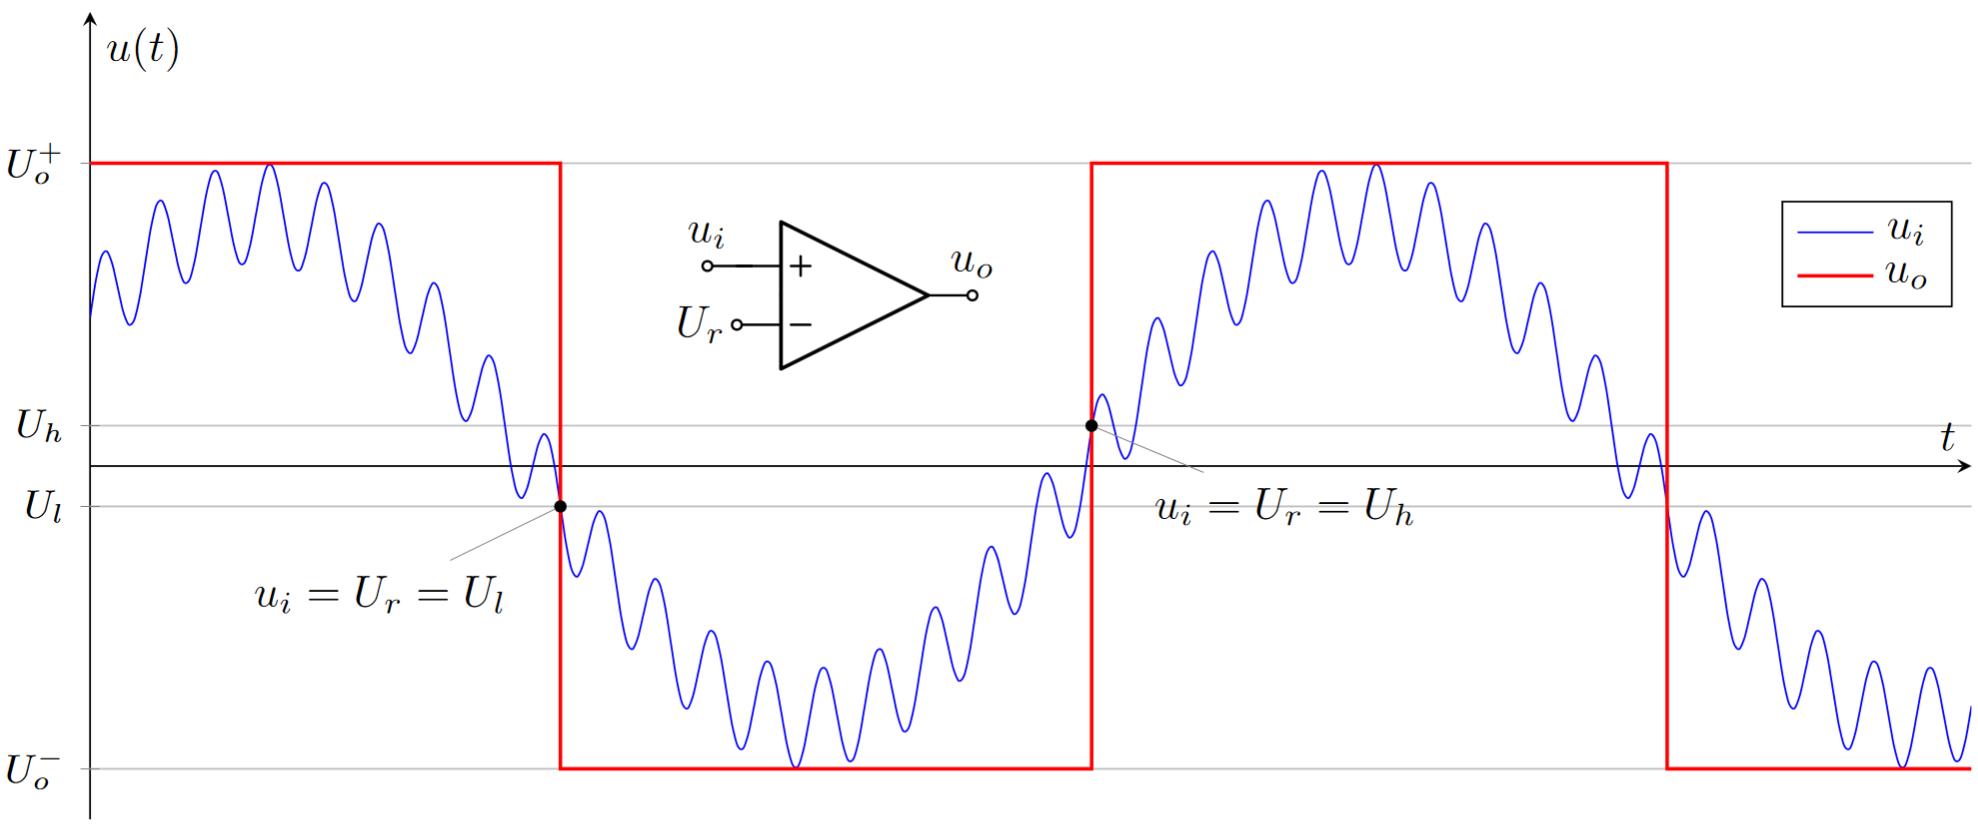
\includegraphics[width=.7\textwidth]{komparator-hyst-graf.PNG}
    \caption{Výstup komparátoru s~hysterezí}
    \label{graf:komp:hyst}
\end{graf}

\subsection*{Invertující komparátor s~hysterezí}
Všimněte si, že invertující komparátor na obr. \ref{fig:invert:komp} skoro vypadá jako neinvertující zesilovač, ale vstupy (+) a~(-) jsou prohozené.

\textbf{Jak to funguje?} Operační zesilovač zesiluje rozdíl na svých vstupech. S~tím, jak obrovské je zesílení samotného zesilovače ($A = 10^6)$, stačí, aby rozdíl mezi vstupy byl jen malilinkatý a~zesilovač jde hned do saturace - na výstup hodí svoje napájecí napětí \underline{$U_o^+$ pro $u_+ > u_-$ nebo $U_o^-$ pro $u_+ < u_-$}.

V momentě, kdy vstupní napětí $u_i$ (shodné s~$u_-$) bude vyšší jak $u_+$, výstup se stáhne dolů ($U_o^-$ pro $u_+ < u_-$) a~OZ dojde do saturace - na výstupu bude záporné napájecí napětí. Díky zavedenému děliči napětí se ale najednou na $u_+$ objeví lehce záporné napětí. Pokud bychom chtěli překlopit výstup nahoru (aby tam bylo $U_o^+$), musíme splnit, že $u_+ > u_-$. Na vstup $u_+$ nám ale teď dělič napětí zavedl trochu záporné napětí. Aby byla splněna podmínka pro překlopení, musíme vstupní signál stáhnout ještě víc do záporna, než je momentálně $u_+$.

\begin{figure}[h!]
    \centering
    \begin{subfigure}{.3\textwidth}
        \centering
        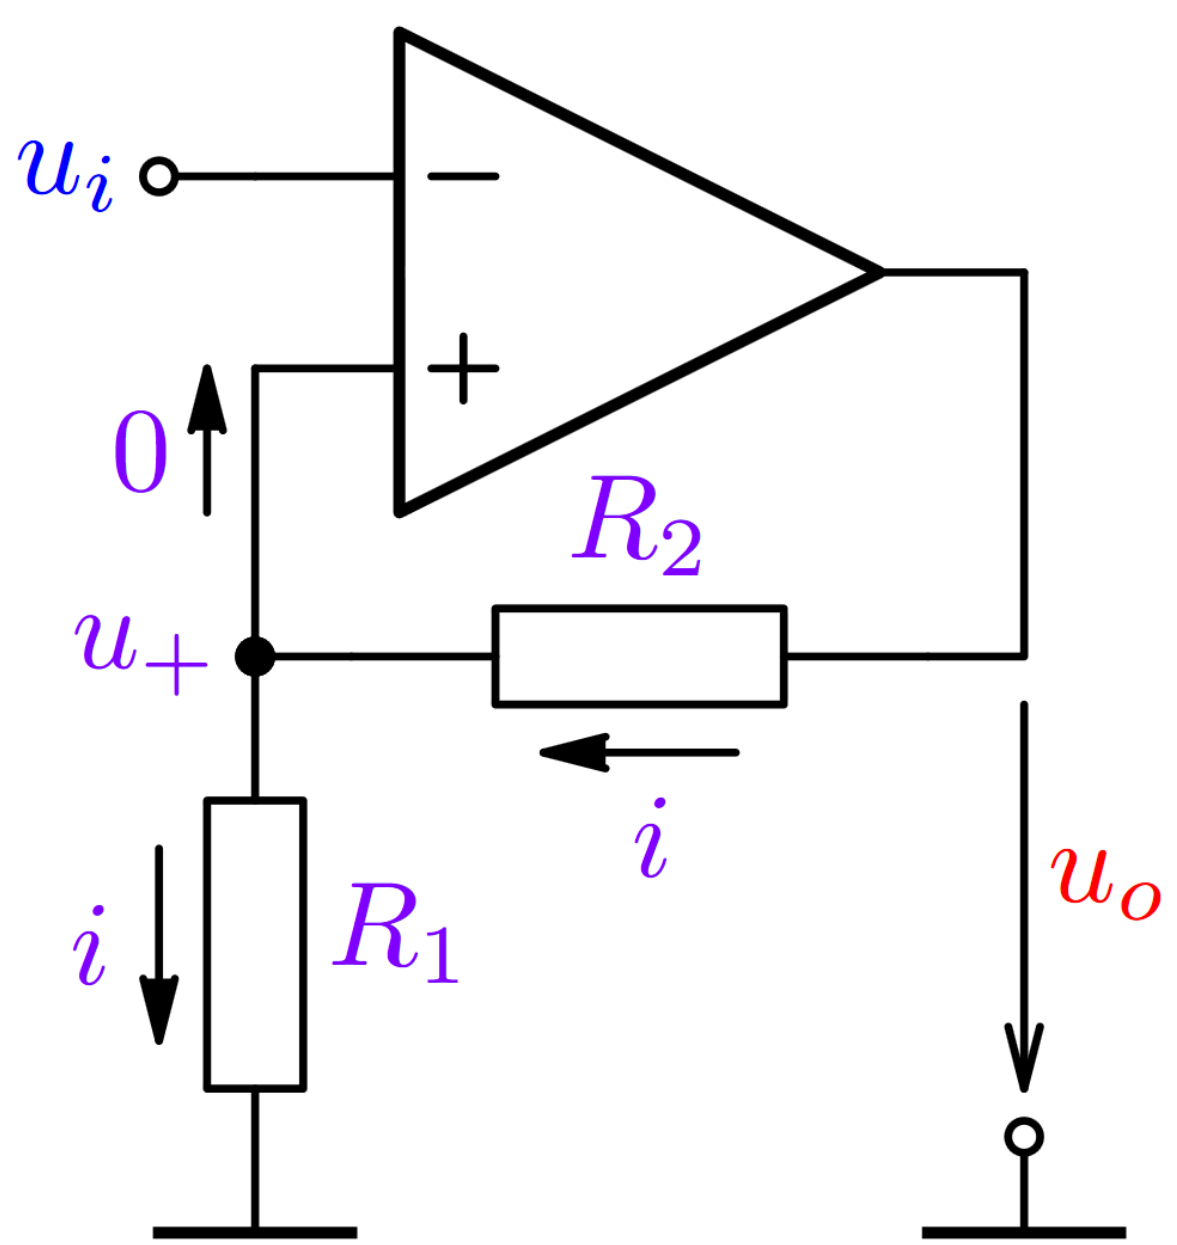
\includegraphics[width=\textwidth]{komparator-invert.PNG}
    \end{subfigure}
    \begin{subfigure}{.65\textwidth}
        \centering
        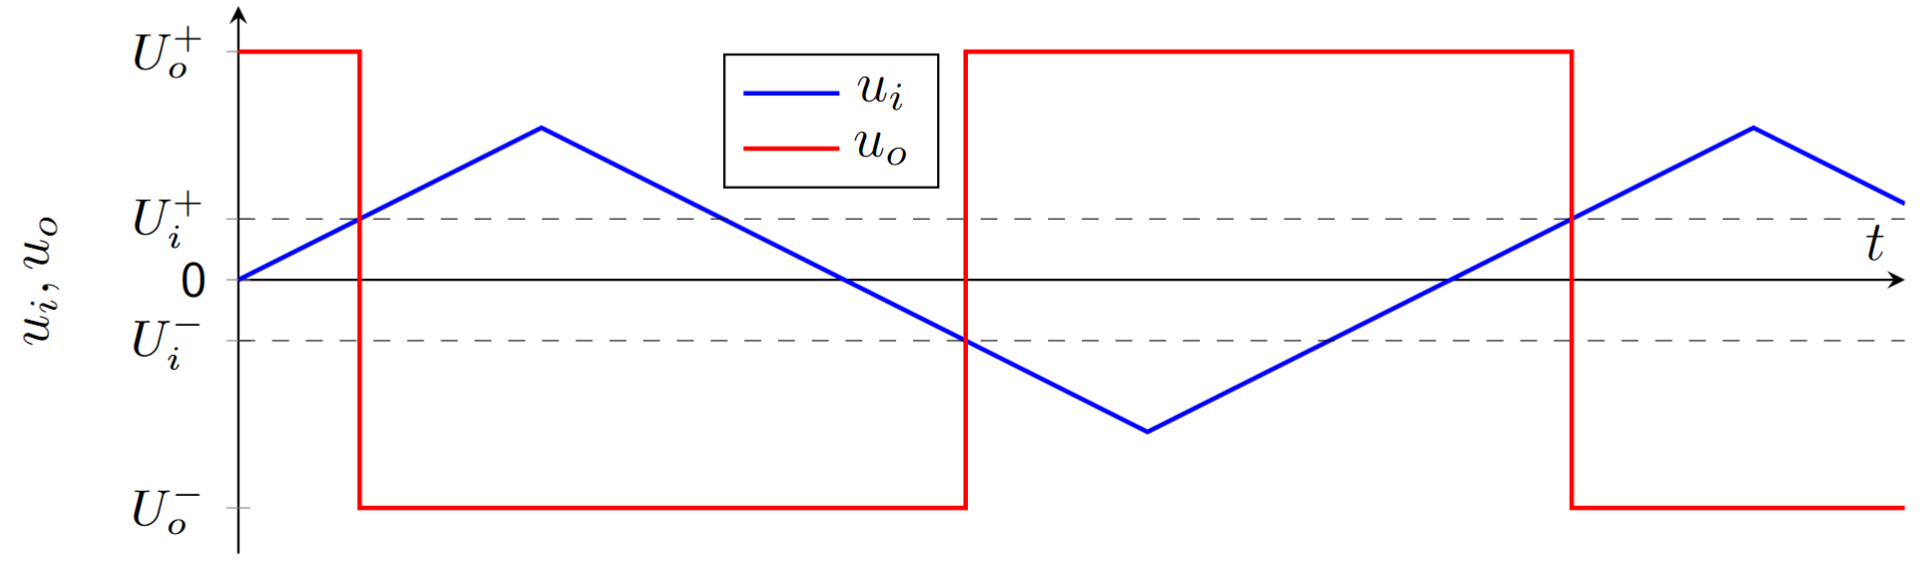
\includegraphics[width=\textwidth]{komparator-invert-graf.PNG}
    \end{subfigure}
    \caption{Schéma a~průběhy invertujícího komaparátoru s~hysterezí}
    \label{fig:invert:komp}
\end{figure}

Z toho nám vycházejí překlápěcí úrovně:\\
\begin{align*}
    U_i^+ &= U_o^+\frac{R_1}{R_1 + R_2},\\
    U_i^- &= U_o^-\frac{R_1}{R_1 + R_2}.\\
\end{align*}





\subsection*{Neinvertující komparátor s~hysterezí}
Všimněte si, že Neinvertující komparátor na obr. \ref{fig:neinvert:komp} skoro vypadá jako invertující zesilovač, ale vstupy (+) a~(-) jsou prohozené.

Operační zesilovač porovnává napětí $u_+$ vůči zemi. Pokud bude $u_+ > 0$, tak $u_o = U_o^+$ (na výstupu bude kladné napájecí napětí). Pokud $u_+ < 0$, tak $u_o = U_o^-$ (na výstupu bude záporné napájecí napětí).

Pokud bude na výstupu kladné napětí, tak sám operák si do svého vstupu přidává jistý proud. Čiže pokud se na vstupu komparátoru objeví dotatečné napětí na překlopení, operák si na vstup $u_+$ ještě přidá, aby se v~tomto překlopeném stavu zafixoval. Pokud bychom chtěli komparátor překlopit dolů s~zápornému napájecímu napětí, musíme na vstup komparátoru dát ještě o~něco víc záporný signál, abychom přebili to, co si tam pouští momentálně nahoru překlopený OZ.

\begin{figure}[h!]
    \centering
    \begin{subfigure}{.3\textwidth}
        \centering
        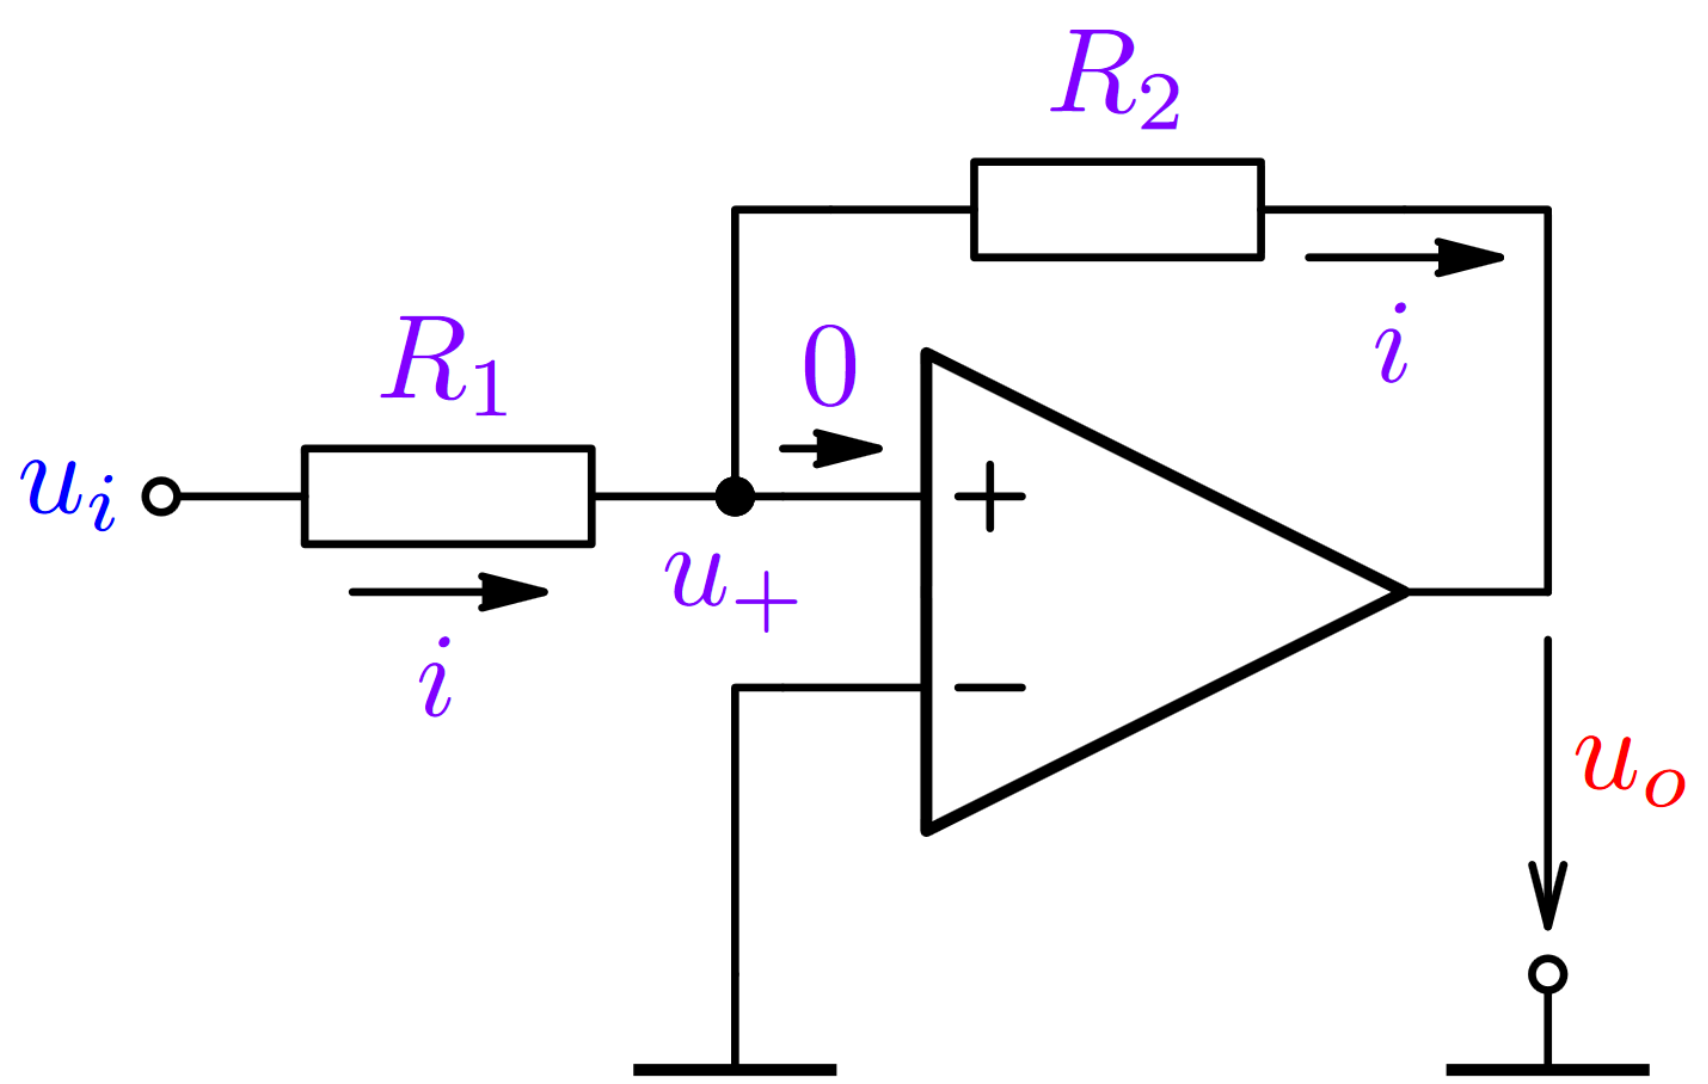
\includegraphics[width=\textwidth]{komparator-noninvert.PNG}
    \end{subfigure}
    \begin{subfigure}{.65\textwidth}
        \centering
        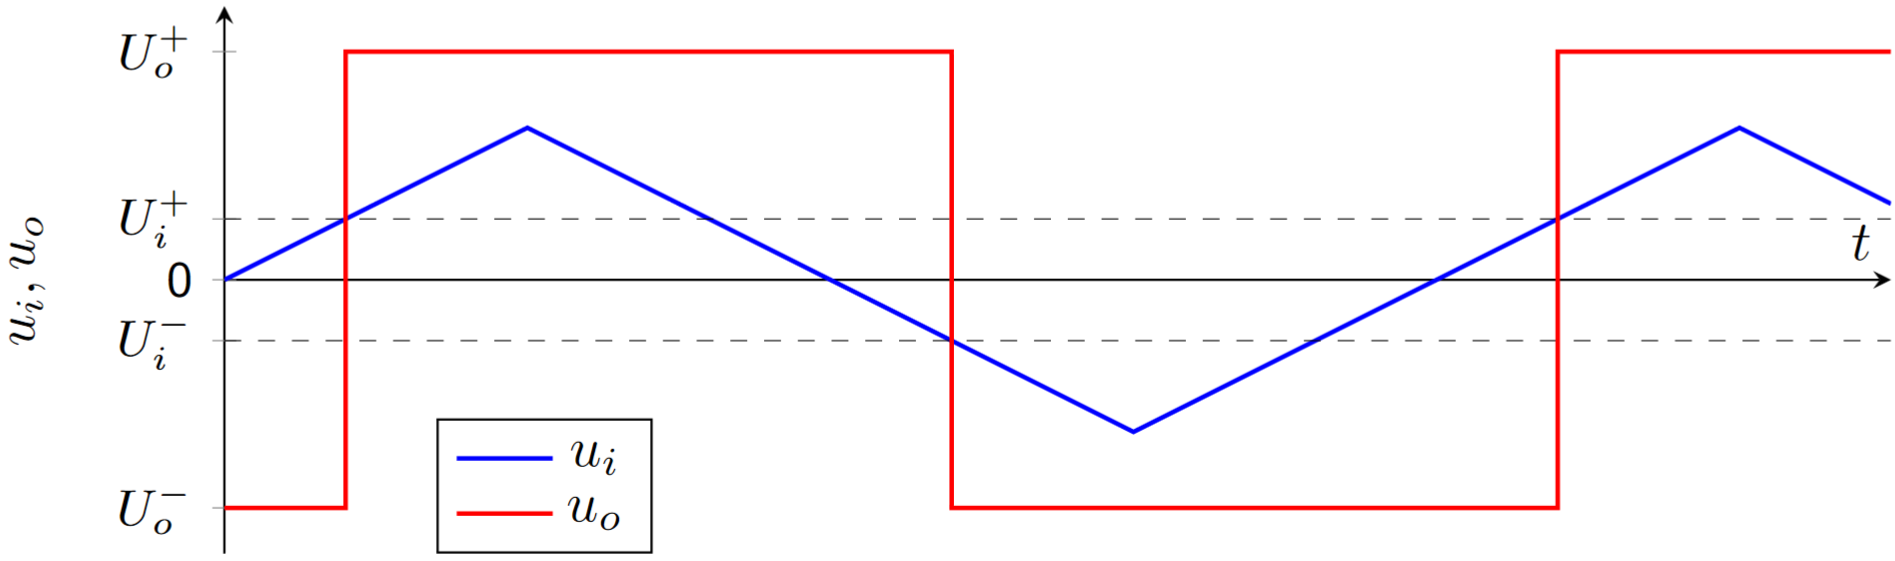
\includegraphics[width=\textwidth]{komparator-noninvert-graf.PNG}
    \end{subfigure}
    \caption{Schéma a~průběhy neinvertujícího komaparátoru s~hysterezí}
    \label{fig:neinvert:komp}
\end{figure}

\textbf{Analogie ze života}\\
Představte si, že jste v~hospodě a~nějaký vnitřní ukazatel vám zabliká, pokud se akorát tak dostanete na hladinu alkoholu, po které vám bude ráno blbě. Hystereze v~tomto případě znamená, že do sebe ještě kopnete další tři panáky, abyste si pošéfovali, že jste tuto hladinu překročili dostatečně. Pokud se ale budete chtít vrátit zpět pod hladinku např. pitím vody, budete muset přepít ještě ty tři panáky. Stejně jako signál do komparátoru musí přebít to, co si tam OZ sám pouští na uzel $u_+$ skrze $R_2$.
















%17
\section{Nakreslete principiální zapojení obvodu S\&H (Sample and Hold) s~OZ a~popište jeho funkci, výhody/ nevýhody a~použití.}\href[pdfnewwindow=true]{http://hippo.feld.cvut.cz/vyuka/soubory/ElektronickeObvody.pdf#section.11.15}{\textit{Odkaz na odpovídající kapitolu v Hospodkových skriptách}}

\textbf{Motivace}: velice často využívaný obvod při A/D převodu. Pokud je spínač $S$ sepnutý, napětí na kondenzátoru $C$ odpovídá vstupnímu signálu. V~momentě rozepnutí spínače zůstane uložena na kondenzátoru poslední hodnota napětí. Díky tomu můžeme \uv{zmrazit} napětí v~daném čase, uložit a~dále s~ním pracovat - např. změřit.

Operační zesilovač je zde využit jako sledovač napětí viz schéma \ref{sch:sledovac}. Jak říká mantra - do vstupu OZ nic neteče. A~tedy kondenzátor ve sch. \ref{sch:sah} se nebude nijak vybíjet.\footnote{V praxi do vstupu OZ proud skutečně teče, ale jedná se řádově \tmu A~až fA.}

\begin{schema}
    \centering
    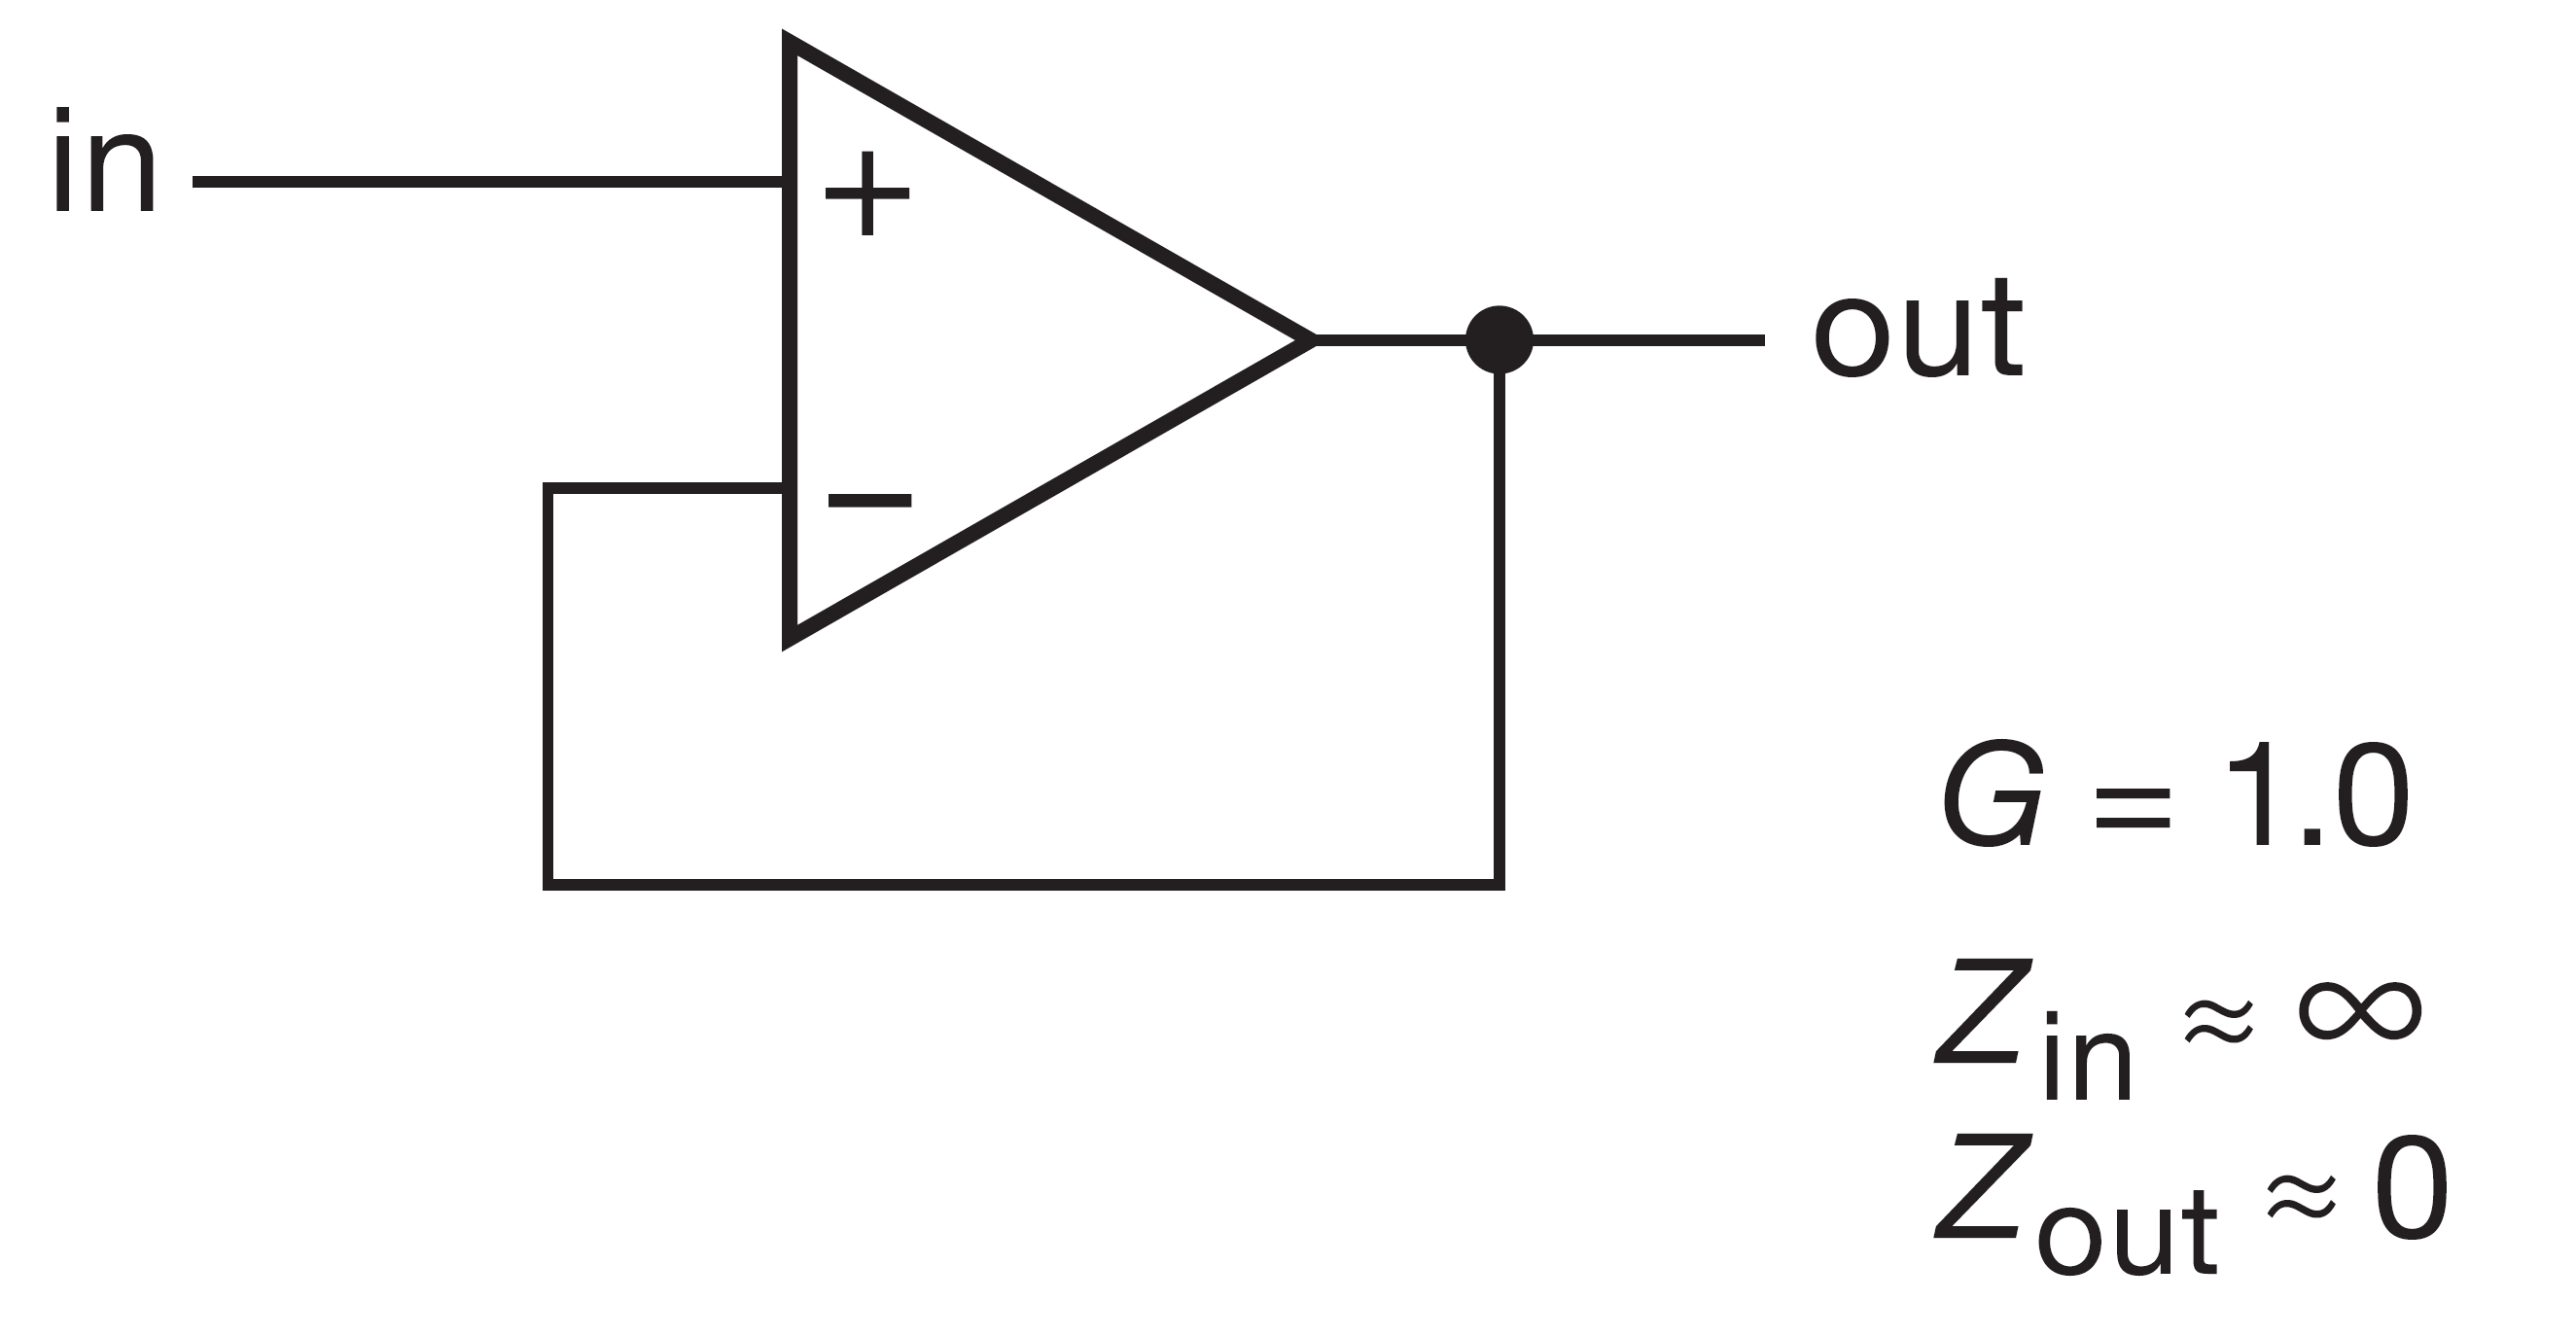
\includegraphics[width=.5\textwidth]{voltage-follower.PNG}
    \caption{Operační zesilovač zapojený jako sledovač napětí}
    \label{sch:sledovac}
\end{schema}

\begin{schema}
    \centering
    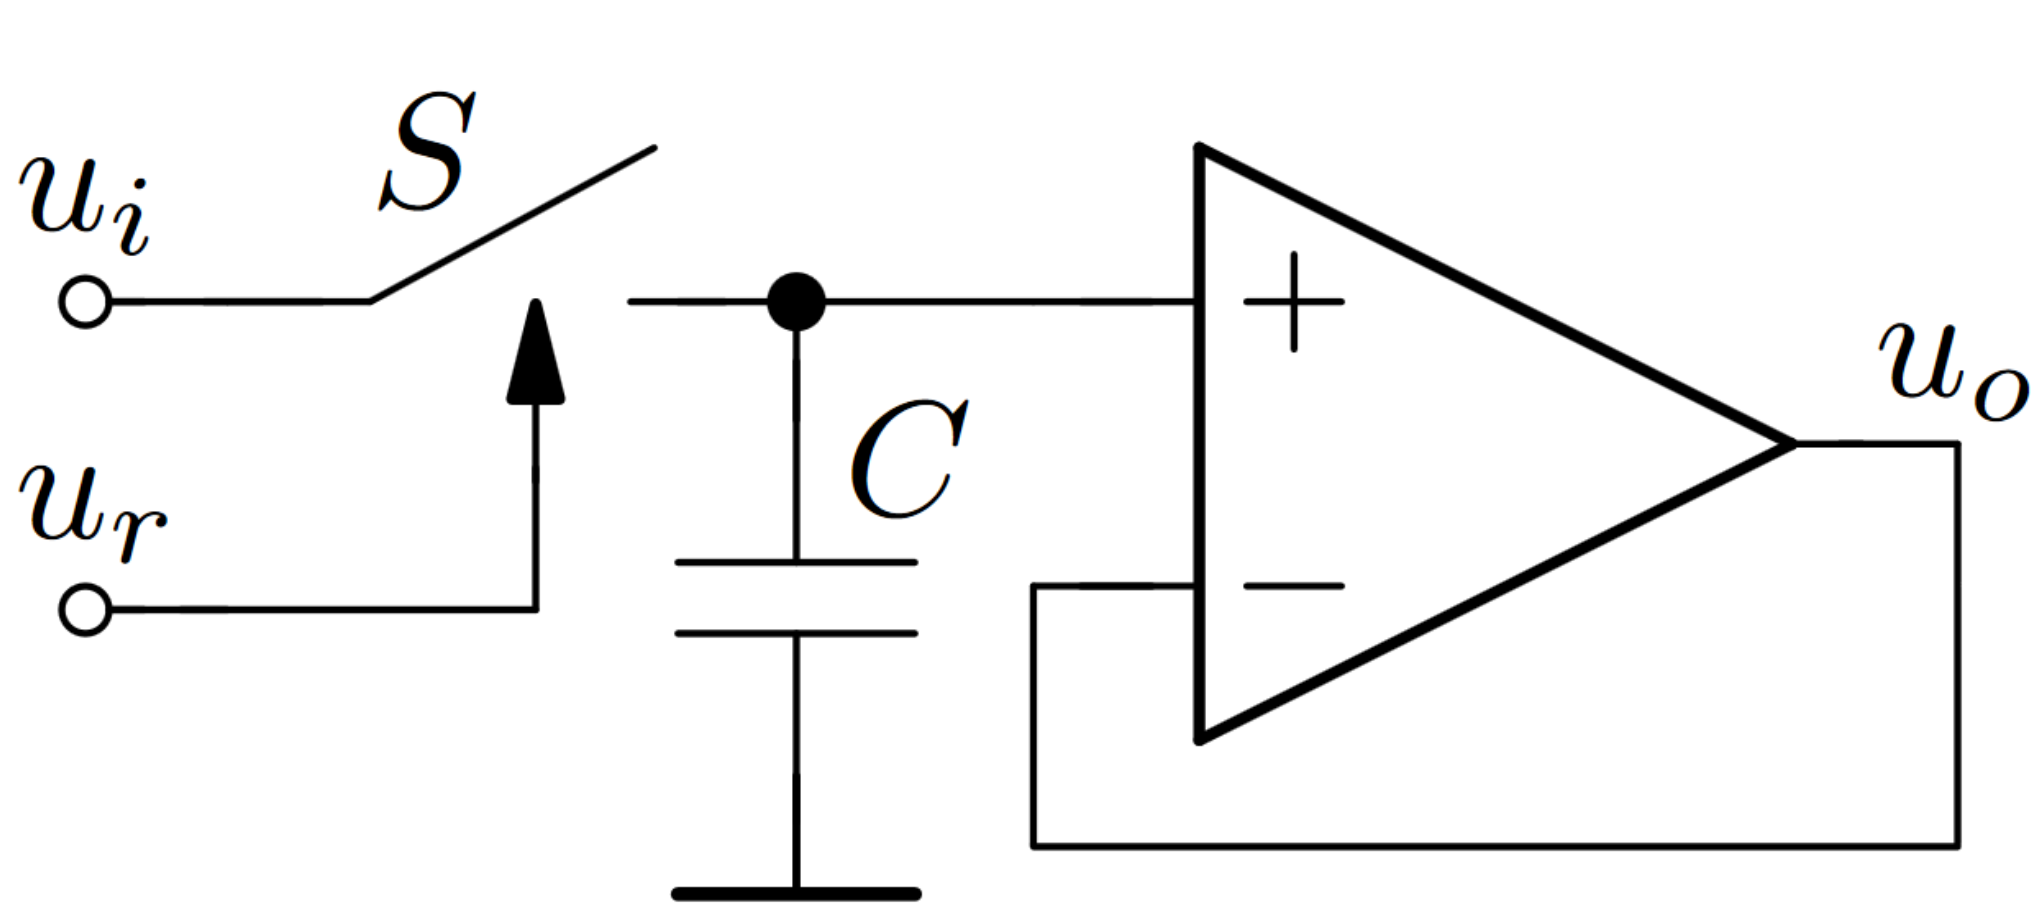
\includegraphics[width=.5\textwidth]{sample_hold.PNG}
    \caption{Operační zesilovač zapojený jako Sample and Hold}
    \label{sch:sah}
\end{schema}

V praxi se přidává ještě jeden sledovač napětí mezi spínač a~kondenzátor, který řídí napětí na kondenzátoru. Díky tomu nezatěžujeme měřený signál, který by jinak musel nabíjek kondík. Ještě víc v~praxi se použije čip, kde je to všechno pohromadě.
\\
\hrule%-----------------------------------------












\newpage
%18
\section{Nakreslete principiální zapojení můstkového oscilátoru. Jaké typy článků (modulových charakteristik) jsou zapojeny v~záporné nebo kladné ZV? Co musí být dodrženo, aby výstupní kmity byly harmonické?}
\begin{schema}[h!]
    \centering
    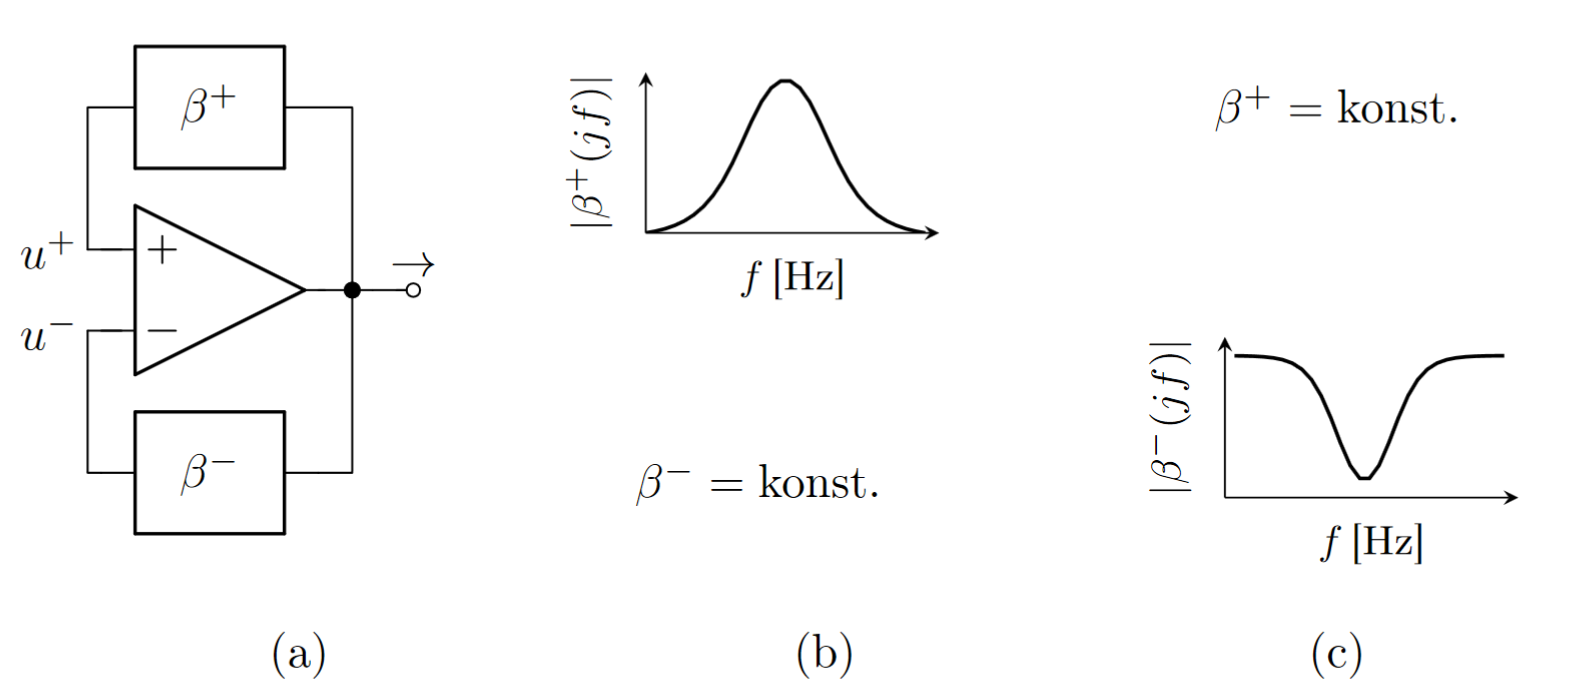
\includegraphics[width=.9\textwidth]{mustkovy-oscilator.PNG}
    \caption{Principiální blokové schéma můstkového oscilátoru (a) s~kmitočtově závislým členem v~kladné (b) nebo záporné (c) zpětné vazbě}
    \label{sch:mustkovy:oscilator}
\end{schema}

Ve zpětné vazbě je zapojena buď pásmová propust (b) nebo pásmová zádrž (c)

\begin{graf}[h!]
    \centering
    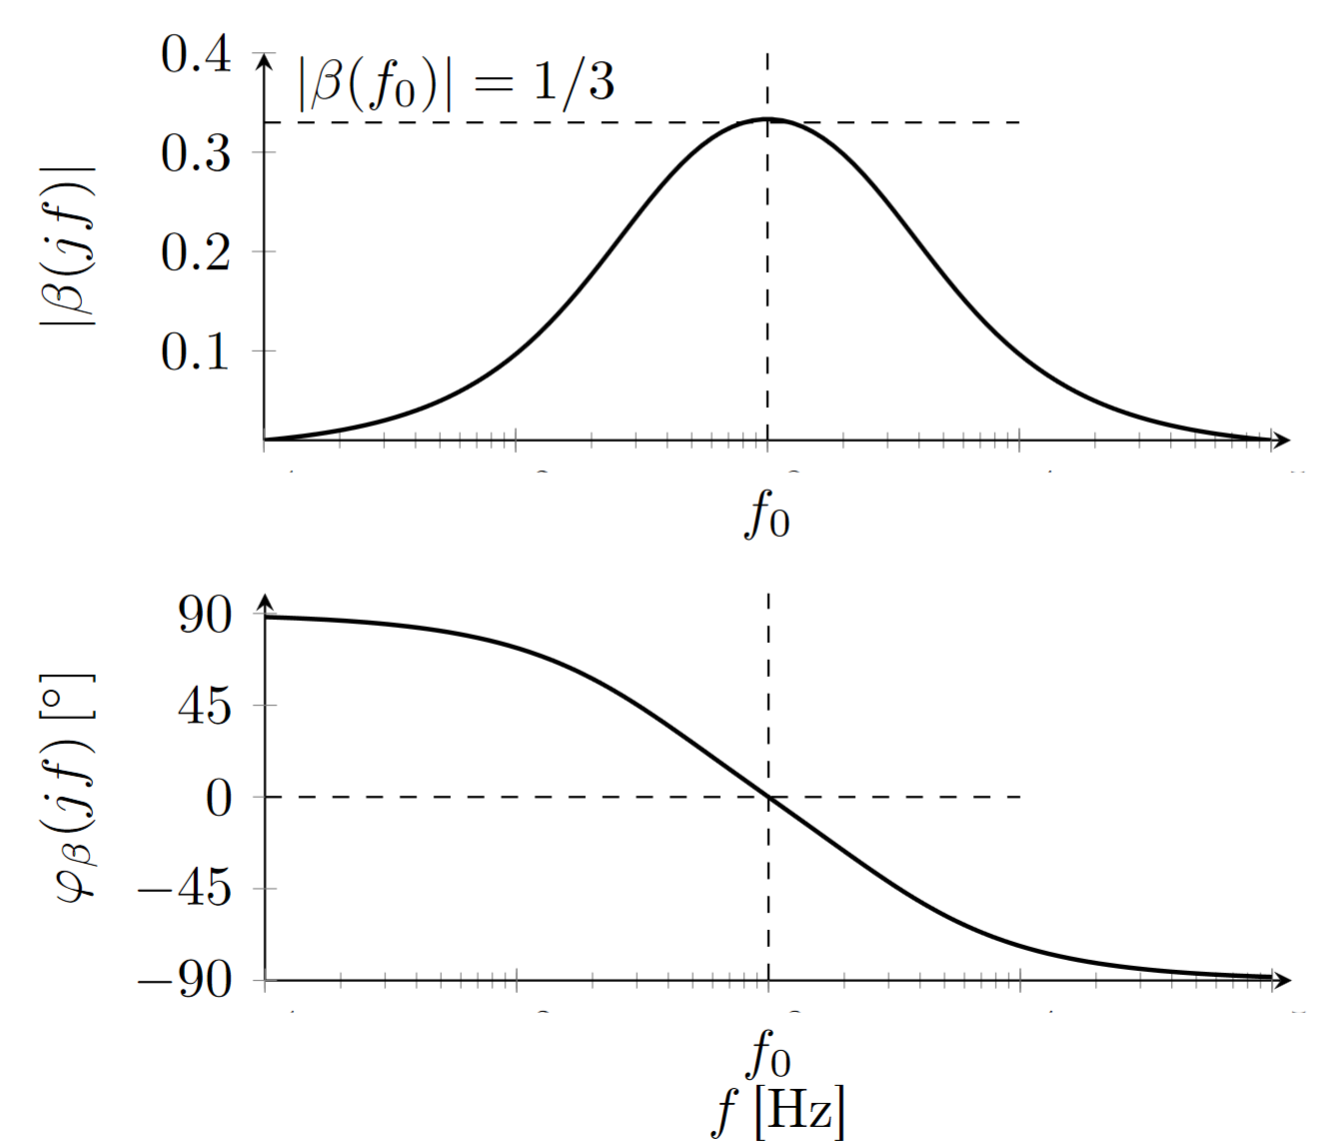
\includegraphics[width = .5\textwidth]{modulova-charakteristika-zv-clanku-oscilator.PNG}
    \caption{Modulová a~fázová charakteristika zpětnovazebního článku}
    \label{graf:osc:modul:charstka}
\end{graf}







%19
\section{Nakreslete zapojení astabilního klopného obvodu s~komparátorem (OZ). Popište princip jeho činnosti a~nakreslete časové průběhy důležitých veličin.}
\textbf{Motivace} příjemný a~jednoduchý obvod na generování obdélníkového signálu. S~trochou poladění lze využít i~jako napětím řízený oscilátor (využití v~syntetizátorech).

\begin{figure}[h!]
    \centering
    \begin{subfigure}{.4\textwidth}
        \centering
        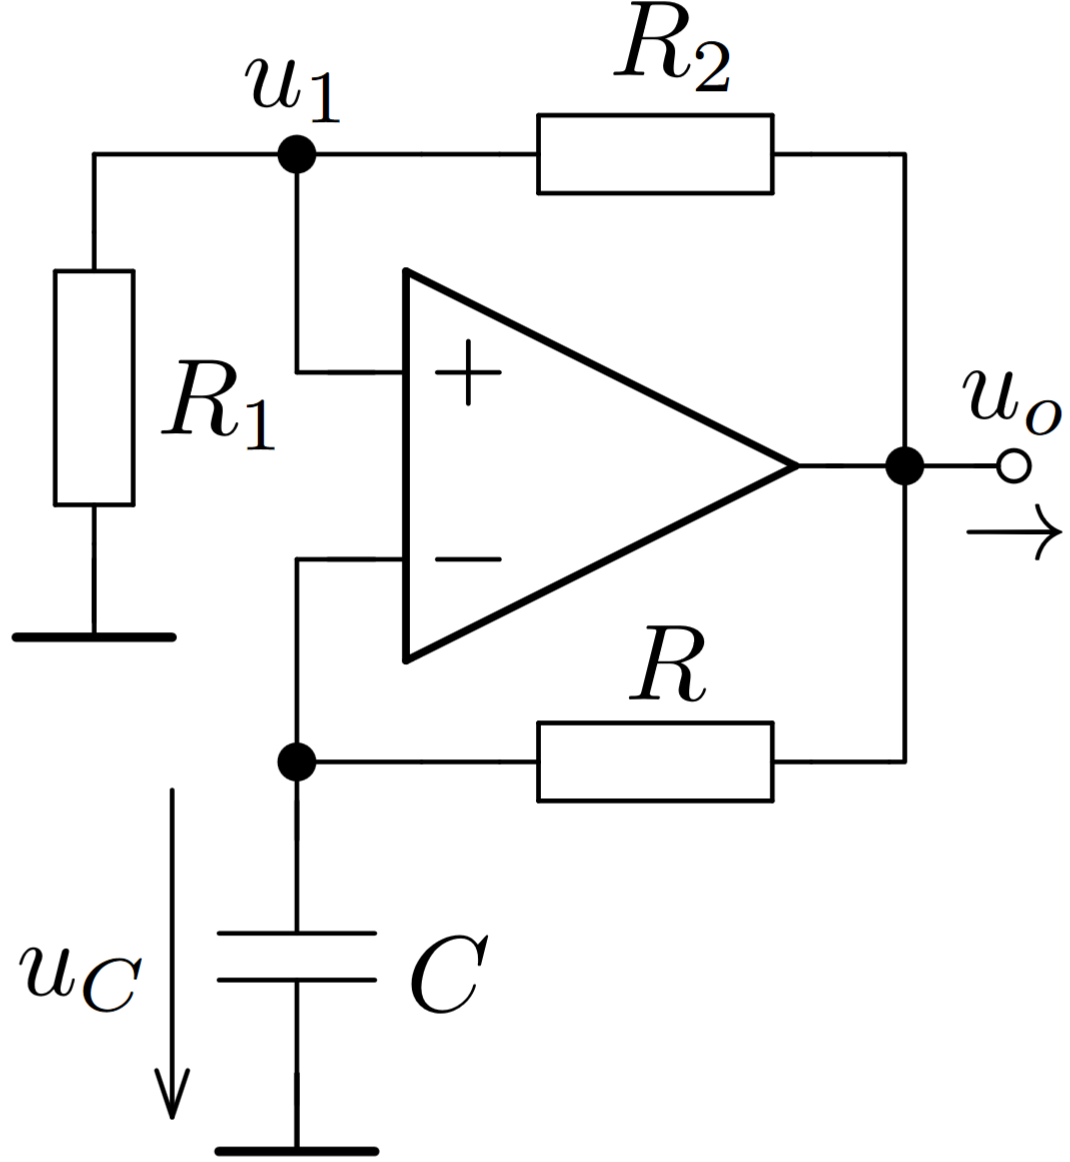
\includegraphics[width=.8\textwidth]{astab_klop.PNG}
        \caption{Zapojení s~operačním zesilovačem zapojeným jako invertující komparátor}
        \label{sch:astab:kl}
    \end{subfigure}
    \hspace{2em}% Space between image A~and B
    \begin{subfigure}{.4\textwidth}
        \centering
        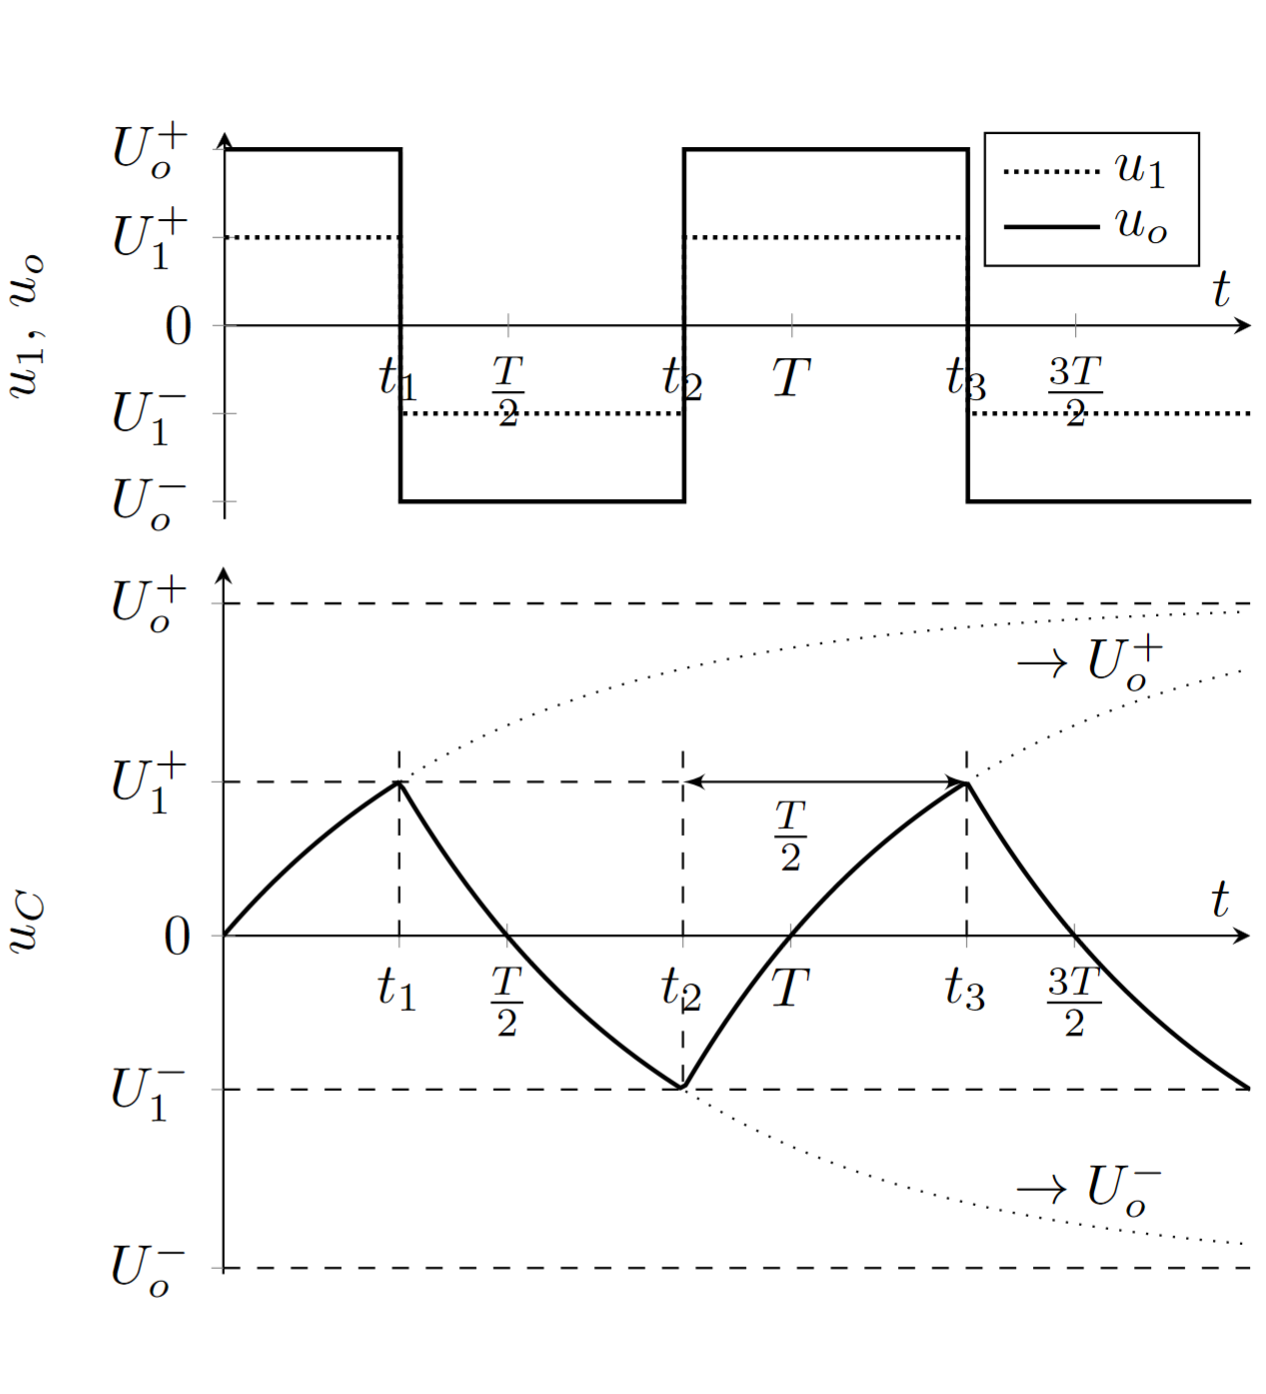
\includegraphics[width =.8\textwidth]{astab_klop-prubehy.PNG}
        \caption{Průběhy napětí na výstupu OZ a~na kondenzátoru}
        \label{graf:astab:kl}
    \end{subfigure}
    \caption{Astabilní klopný obvod}
\end{figure}



\textbf{A jak to teda funguje?} OZ jde vždy do saturace - tedy na výstupu je buď kladné napájecí napětí $U_o^+$ nebo záporné napájecí napětí $U_o^-$. Kladné napájecí napětí se na výstup dostane, pokud je na neinvertujícím (+) vstupu vyšší napětí než na invertujícím (-) vstupu: 

\begin{center}
    $U_o^+$ pro $u_+ > u_-$ nebo $U_o^-$ pro $u_+ < u_-$.
\end{center}

Než začneme, všiměme si děliče napětí tvořeného rezistory $R_1$ a~$R_2$. Výstupní napětí tohoto děliče $u_1 = U_o \frac{R_1}{R_1 + R_2}$ nám bude udávat komparační úroveň pro napětí na kondenzátoru.

Začneme s~výstupem, na němž je kladné napájecí napěí a~vybitým kondenzátorem.

\begin{enumerate}
    \item na $u_o$ je kladné napájecí napětí, na neinvertujícím (+) vstupu je výstupní napětí z~děliče $R_1, R_2$.
    \item Kondenzátor se začne skrze rezistor $R$ nabíjet a~jeho rostoucí napětí je vidět na spodním průběhu v~grafu \ref{graf:astab:kl}.
    \item V~momentě, kdy se napětí na kondenzátoru dostane na stejnou hodnotu, jako je napětí na děliči nahoře, obvod se překlopí. To proto, že na invertujícím vstupu je vyšší napětí jak na neinvertujícím a~tedy výstup operáku jde dolů na hodnotu záporného napájecího napětí.
    \item Na výstupu je záporné napájecí napětí a~díky děliči vedoucí na neinvertující vstup se záporné napětí objeví i~tam.
    \item Kondenzátor se začne vybíjet skrze $R$, jak je dále vidět v~dolním průběhu ve grafu \ref{graf:astab:kl}.
    \item V~momentě, kdy se kondenzátor vybije tak moc do záporna, že napětí na něm spadne pod výstup děliče, najednou máme na invertujícím vstupu menší naptětí jak na neinvertujícím a~operák se překlopí a~na výstupu OZ se objeví kladné napájecí napětí.
\end{enumerate}
Toto je jedna perioda kmitu, nyní se kondenzítor začne nabíjet a~budeme čekat, než napětí na něm přeleze hodnotu napětí z~děliče.






%20
\section{Nakreslete zapojení generátoru funkcí {trojúhelníkového a~obdélníkového průběhu}. Popište princip jeho činnosti a~nakreslete časové průběhy důležitých veličin.}

\textbf{Motivace}: další užitečné schéma. A~nejen to, dokonce je tvořen z~bloků, které jsme již probírali. Vše se krásně spojuje dohromady!

\textbf{Popis bloků }- činnost krok za krokem bude následovat níže\\
V levé části je zapojení integrátoru s~OZ (viz kapitola \ref{chap:integrator}). Proud protékající skrze rezistor $R$ musí protékat také skrze kondík $C$. Výstup levého OZ se bude korigovat tak, aby tato podmínka byla zajištěna. Pouze tak dosáhne OZ stejného napětí na svých vstupech - v~našem případě 0~V. Při konstantním proudu skrze kondenzátor bude napětí na něm lineárně stoupat/klesat. Zde se rodí trojúhelníkový průběh.

Pozor! Pokud bude téct rezistorem $R$ proud doprava, musí OZ tento proud také odčerpávat. To zajistí tím, že bude výstup tahat do záporna. Tedy je to invertující integrátor.

Operační zesilovač vpravo se chová jako neinvertující komparátor (viz kapitola \ref{chap:komp}). V~momentě, kdy napětí na výstupu levého OZ překročí komparační úroveň, hodí se na výstup OZ odpovídající napětí.
\begin{schema}[h!]
    \centering
    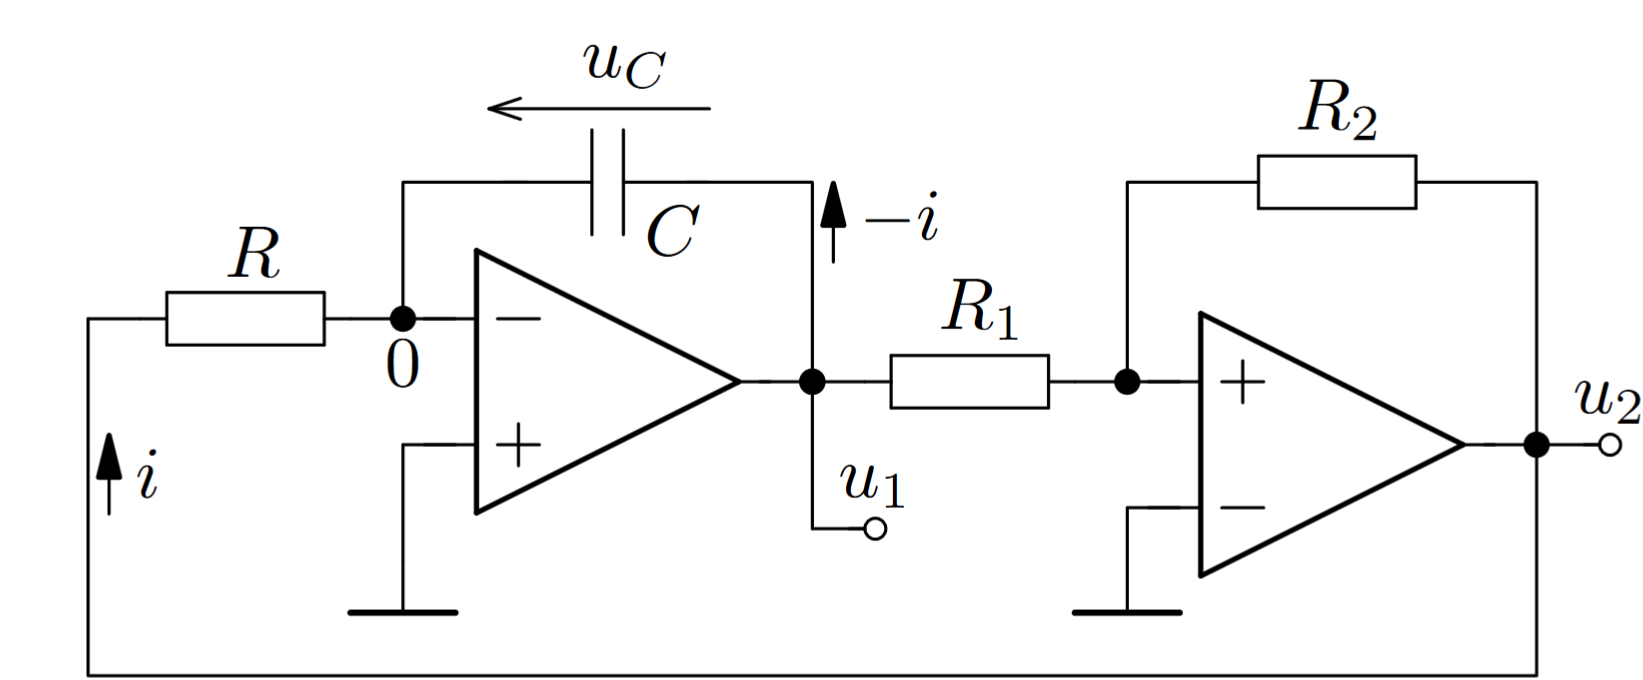
\includegraphics[width=.7\textwidth]{gen_funct.PNG}
    \caption{Generátor funkcí s~operačním zesilovačem}
    \label{sch:gen:fci}
\end{schema}

\textbf{A jak to tedy funguje?} Dejme tomu, že na výstupu komparátoru (pravý OZ) bude kladné napájecí napětí:
\begin{enumerate}
    \item Kladné napětí se objeví i~před rezistorem $R$ a~proud poteče doprava. Aby mohl téct proud dále skrz kondenzátor, musí jít výstup levého OZ do záporna (jak je vidět v~grafu \ref{graf:astab:kl})
    \item Díky hysterezi zavedené rezistory $R_1$ a~$R_2$ musí jít výstup levého OZ ještě o~něco víc do záporna, aby se vykompenzovalo to, že výstup komparátoru skrze $R_2$ tahá svůj neinvertující (+) vstup nahoru. (Analogie z~hospody zmíněná dříve.)
    \item V~momentě, kdy bude napětí dost záporné se komparátor překlopí a~na výstup hodí záporné napájecí napětí. Toto napětí se objeví i~na rezistoru $R$ a~začné téct proud doleva. Tento proud začne zvyšovat napětí na kondenzátoru a~výstup levého OZ se začne zvyšovat.
    \item Zvyšovat do té doby, než se dostane na komparační úroveň pravého komparátoru. V~ten moment se výstup komparátoru překlopí a~vše začne odznova.
\end{enumerate}

\begin{graf}[h!]
    \centering
    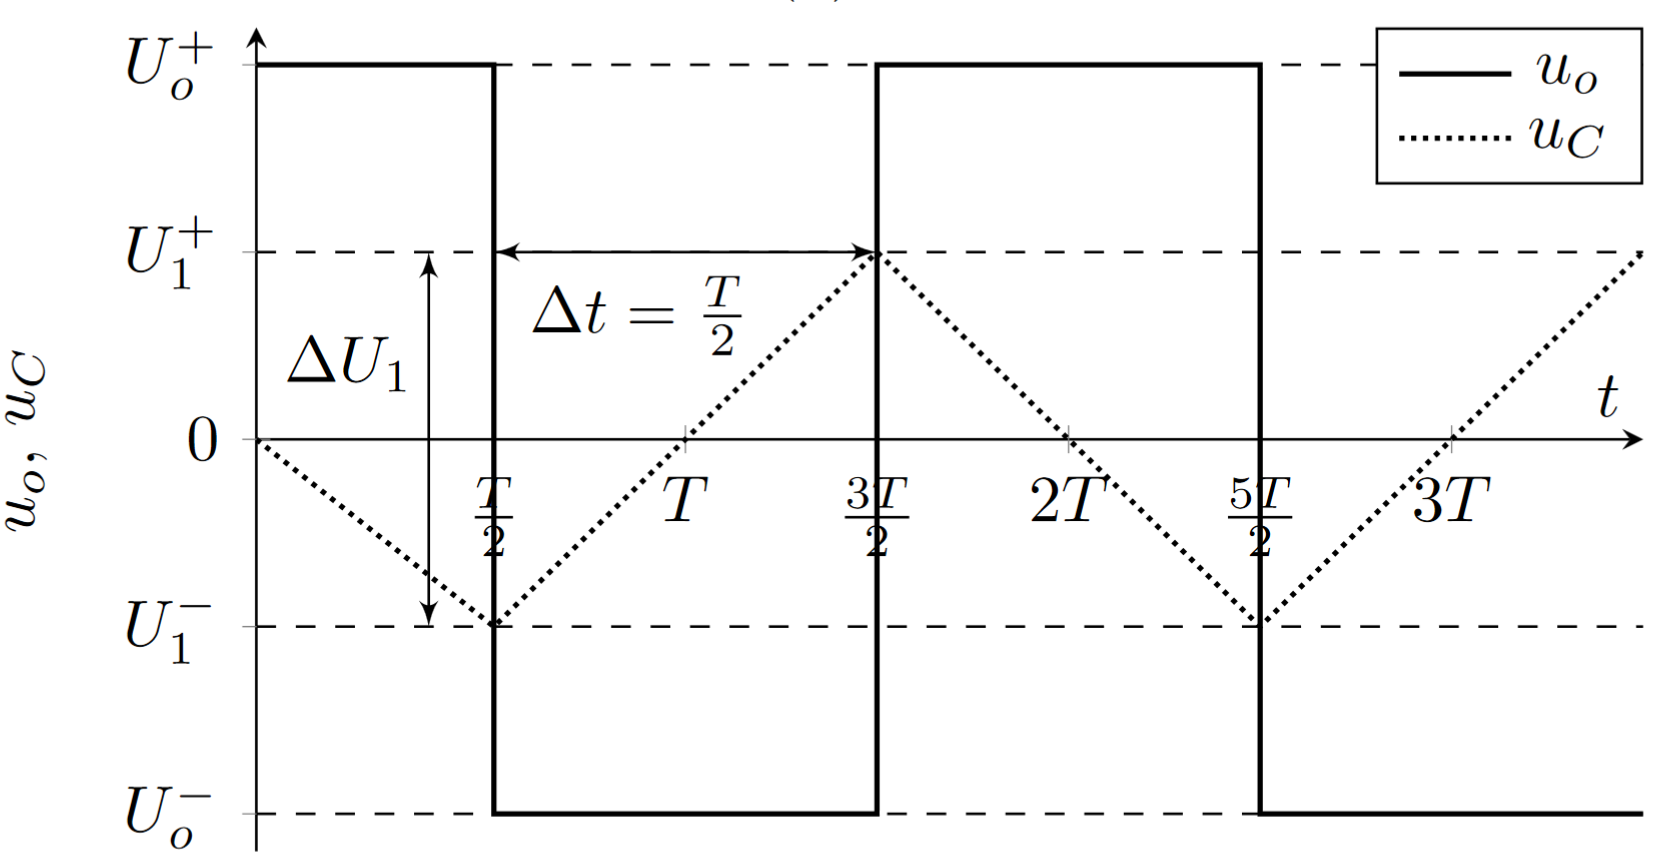
\includegraphics[width = .75\textwidth]{gen_funct-graf.PNG}
    \caption{Průběhy na výstupech operačních zesilovačů}
    \label{graf:gen:fci}
\end{graf}









%21
\section{Nakreslete blokové schéma fázového závěsu, popište princip jeho činnosti a~vysvětlete pojmy pásmo zachycení a~pásmo zadržení. Dále nakreslete blokové schéma kmitočtové syntézy s~fázovým závěsem a~odvoďte vztah pro kmitočet výstupního signálu.}
\textbf{Motivace}: násobení frekvencí. Mluvil o~tom Záhlava, tak to asi bude docela v~praxi využitelné.

\begin{schema}[h!]
    \centering
    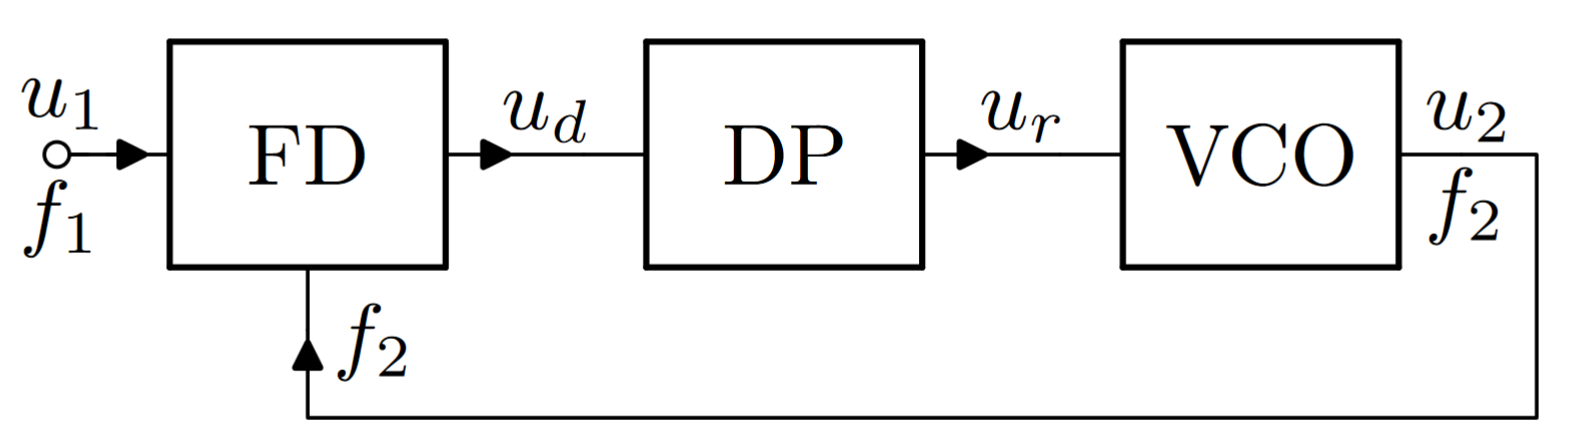
\includegraphics[width=.6\textwidth]{fazovy_zaves.PNG}
    \caption{Blokové schéma fázového závěsu}
    \label{sch:faz:zaves}
\end{schema}

Fázový závěs je tvořen třemi bloky:
\begin{itemize}
    \item \textbf{Fázový detektor}, který porovnává fázi vstupního signálu a~zpětnovazebního signálu
    \item \textbf{Dolní propust} - prostě filtru
    \item \textbf{Napětím řízený oscilátor} - oscilátor, jehož frekvence se nastavuje napětím.
\end{itemize}

Napětí $u_d$ je dáno rozdílem fází vstupního a~zpětnovazebního signálu. Tím se mění frekvence VCO tak, aby byla shodná se vstupním signálem.

Hodně cool věc je, že můžeme jednoduše dělit frekvenci ve zpětné vazbě. Díky tomu ošálíme fázový detektor a~ten bude oscilátoru přikazovat, aby dělal násobně vyšší frekvenci, aby byla ta vydělená shodná s~frekvencí vstupního signálu.

\begin{graf}[h!]
    \centering
    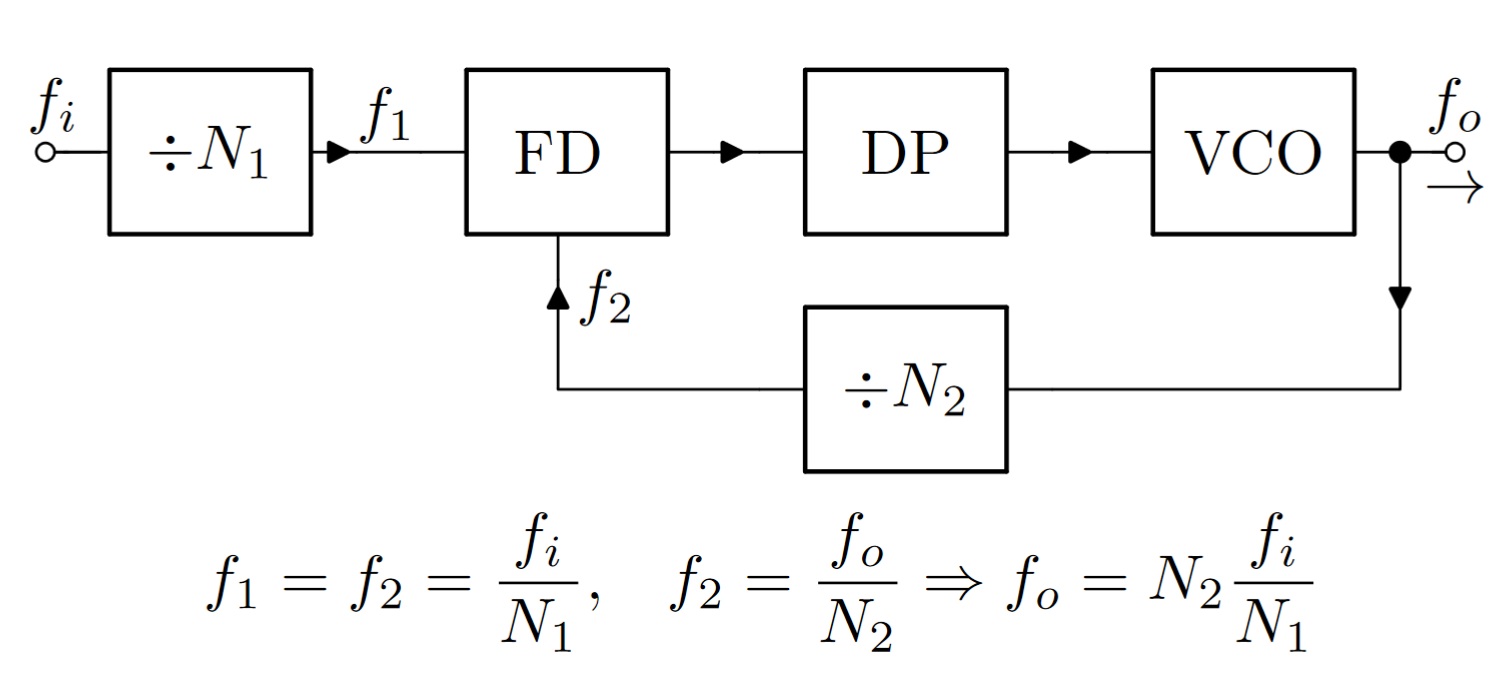
\includegraphics[width = .6\textwidth]{fazovy_zaves-deleni.PNG}
\end{graf}
Cool, co?

\subsection*{Pásmo zadržení}
Tomu nerozumím, ale hospodka má dva pěkný grafíky, tak třeba pomůžou a~něco z~nich vykoukáte:
\begin{graf}[h!]
    \centering
    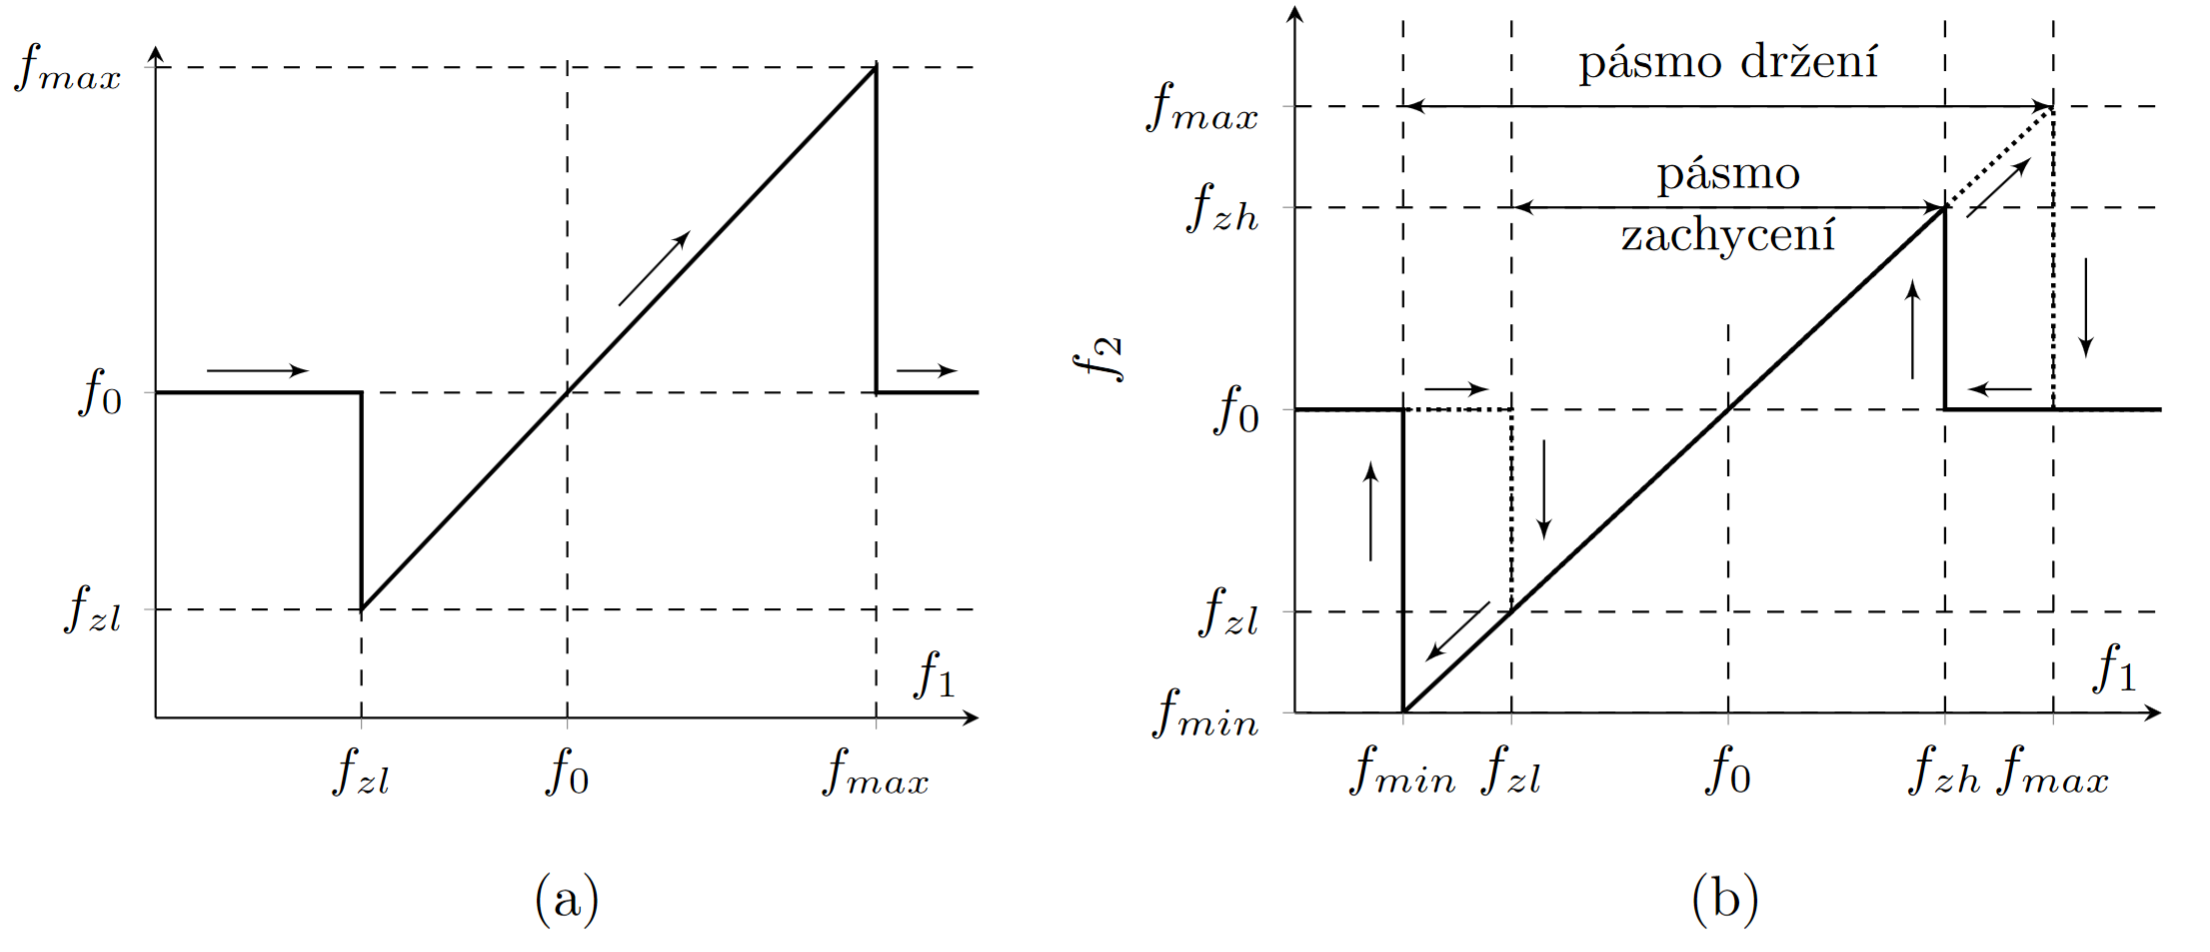
\includegraphics[width=\textwidth]{pasmo_zadrzeni.PNG}
    \caption{Závislost výstupního kmitočtu $f_2$ na vstupním kmitočtu $f_1$ při přelaďování $f_1$ zdola (a) a~shora (b)}
    \label{graf:pasmo:zadrzeni}
\end{graf}

Snad to nebude ve zkoušce...
 \\






\hrule%-----------------------------------------
%22
\section{Nakreslete základní zapojení s~bipolárním/unipolárním tranzistorem jako spínačem pro buzení uzemněné/neuzemněné LED, resp. odporové/indukční zátěže. Určete vztah pro výpočet a~volbu uvedených komponent pro známý proud zátěží $I_\text{z}$ v~ustáleném stavu a~dané úrovně řídícího napětí}
\textbf{Motivace}: můžeme si ukazovat stovky typů zesilovačů, ale stejně je ve výsledku tranzistor nejvíce využíván jako spínač. 

Spínání se dělí na \textit{low-side}, kde tranzistorem dovolujeme, aby odtekl proud do země a~na \textit{high-side}, kde pomocí tranzistoru přivádíme napájecí napětí do zátěže.

\begin{schema}[h!]
    \centering
    \includegraphics[width=.9\textwidth]{tranzistory-spinace2.pdf}
    \caption{Základní zapojení tranzistorů jako spínačů ke spínání odporové a~induktivní zátěže}
\end{schema}
Je důležité si uvědomit, že pokud přivedeme napětí na bázi NPN (šipka ven) resp. gate N-kanálového tranzistoru, tak se sepne. 

ALE! U~PNP a~P-kanálových tranzistorů je to naopak. Pokud přivedeme napětí VCC skrze rezistor na bázi, tak se tranzistor uzavře a~nebude vodit. To proto, že nebude žádný úbytek napětí mezi emitorem (to se šipkou dovnitř) a~bází (oba budou připojeny na napájecí napětí). Abychom sepli tranzistor, musíme hodit CTRL vstup na zem. Obdobně pro P-kanálový tranzistor (úplně vpravo). Tento spínač má v~sobě tedy ještě zabudovanou negaci a~spíná při přivedení 0~V.

Proud, který je bipolární tranzistor ochoten pustit z~kolektoru do emitoru je $\beta$-násobek proudu do báze.
\begin{equation*}
    I_\text{C} = \beta I_\text{B}, ~~~I_\text{B} = \frac{V_\text{CTRL} - V_\text{BE}}{R_\text{B}} = \frac{U_\text{CTRL} - 0.7~\text{V}}{R_\text{B}}
\end{equation*}
Tento proud, který je tranzistor ochoten pustit musí být větší, než proud, který cheme, aby tekl zátěží. Aby byl proud limitován pouze rezistorem v~sérii se zátěží a~nebyl limitován tranzistorem.

U unipolárního tranzistoru musíme dávat pozor, aby proud, který je tranzistor ochoten pustit:
\begin{equation*}
    I_\text{D} = \frac{1}{2}k_p \frac{W}{L} (U_\text{GS} - U_\text{T})^2
\end{equation*}
byl větší, než proud, který požadujeme, aby tekl zátěží.

Rezistory u~Gatu MOSFETů jsou pulldown/pullup rezistory, které zajistí, že se na Gatu nenaindukuje náboj, který by otevřel přechod (to se děje velice často a~pokud tam nedáte pulldown/pullup, tak si poserete život).

Pokud jde o~spínání induktivní zátěže, tak je nutné přidat diodu v~závěrném směru. Pokud se rychle změní proud cívkou, naindukuje se na ní napětí v~opačném směru. Tato špička může prorazit tranzistor a~je potřeba paralelní dioda, která tuto špičku pohltí.

\begin{schema}
    \centering
    \includegraphics[width=.7\textwidth]{tranzistory-spinace_driver.PNG}
    \caption{High-side spínání pomocí omezeného rozsahu napětí řídící logiky}
\end{schema}

%23
\section{Nakreslete zapojení jednostupňového zesilovače s~BJT NPN/PNP v~zapojení SE/SB/SC a~podle náhradního linearizovaného schématu odvoďte vztah pro jeho vstupní odpor $R_i$ a~napěťové zesílení $A_u$.}
\textbf{Motivace}: zesilovače aaaaaA!

\subsection*{Společný Emitor}
\href[pdfnewwindow=true]{http://hippo.feld.cvut.cz/vyuka/soubory/ElektronickeObvody.pdf#subsection.14.5.1}{\textit{Odkaz na odpovídající kapitolu v Hospodkových skriptách}}

\begin{figure}[h!]
    \centering
    \includegraphics[height=5cm]{NPN_SE.PNG}
    \caption{Schéma a~náhradní lin. obvod pro zesilovač se společným emitorem\\\centering$u_{be} = u_i,~~i_c=g_mu_{be},~~u_o=-i_c(R_C||R_z)$}
    \label{fig:zes:se}
\end{figure}
\begin{align}
    A_u &\equiv \frac{u_o}{u_i} = \frac{-i_cR_C}{u_{be}} = \frac{R_C}{u_{be}} = \underline{\underline{-g_mR_C}}\\
    R_i &\equiv \frac{u_i}{i_i} = \underline{\underline{r_\pi}}
\end{align}

\subsection*{Společná Báze}
\href[pdfnewwindow=true]{http://hippo.feld.cvut.cz/vyuka/soubory/ElektronickeObvody.pdf#subsection.14.5.3}{\textit{Odkaz na odpovídající kapitolu v Hospodkových skriptách}}
\begin{figure}[h!]
    \centering
    \includegraphics[height=5cm]{NPN_SB.PNG}
    \caption{Schéma a~náhradní lin. obvod pro zesilovač se společnou bází\\\centering$u_{be} = -u_i,~~i_c=-g_mu_i,~~ u_o = -i_c(R_C||R_z)$}
    \label{fig:zes:sb}
\end{figure}
\begin{align}
    A_u &\equiv \frac{u_o}{u_i} = \frac{R_C}{u_{be}} = \underline{\underline{g_mR_c}}\\
    R_i &\equiv \frac{u_i}{i_i} = r_e = \underline{\underline{\frac{r_\pi}{\beta +1}}}
\end{align}

\subsection*{Společný Kolektor (SC)}
\href[pdfnewwindow=true]{http://hippo.feld.cvut.cz/vyuka/soubory/ElektronickeObvody.pdf#subsection.14.5.5}{\textit{Odkaz na odpovídající kapitolu v Hospodkových skriptách}}
\begin{figure}[h!]
    \centering
    \includegraphics[height=5cm]{NPN_SC.PNG}
    \caption{Schéma a~náhradní lin. obvod pro zesilovač se společným kolektorem\\\centering$u_i = u_{be}+u_o,~~i_i = i_b$}
    \label{fig:zes:sc}
\end{figure}
\begin{align}
    A_u &\equiv \frac{u_o}{u_i} = \frac{R_z}{r_e+R_z} \approx \underline{\underline{1}}\\
    R_i &\equiv \frac{u_i}{i_i} = \underline{\underline{\beta R_z}}\\
\end{align}
Napěťové zesílení $1$, ale proudové zesílení vysoké. Jedná se o~tzv. \textit{napěťový sledovač}. Vstupní odpor (odpor, co vidí signál, když jde do báze) je veliký.




%24
\section{Nakreslete zapojení jednostupňového zesilovače s~MOSFET s~indukovaným kanálem typu N/P v~zapojení SS/SG/SD a~podle náhradního linearizovaného schématu odvoďte vztah pro jeho vstupní odpor a~napěťové zesílení.}

\subsection*{Společný Source}
\href[pdfnewwindow=true]{http://hippo.feld.cvut.cz/vyuka/soubory/ElektronickeObvody.pdf#subsection.14.5.2}{\textit{Odkaz na odpovídající kapitolu v Hospodkových skriptách}}

\begin{figure}[h!]
    \centering
    \includegraphics[height=5cm]{NMOS-SS.PNG}
    \caption{Schéma a~náhradní lin. obvod pro zesilovač se společným sourcem\\\centering$u_{gs} = u_i,~~i_d = g_mu_{gs},~~u_o = -i_d(R_C||R_z)$. Jelikož se jedná o~MOSFET, tak do gatu nic neteče, tedy $i_i=0$}
    \label{fig:zes:ss}
\end{figure}
\begin{align}
    A_u &\equiv \frac{u_o}{u_i} = \frac{i_dR_D}{u_{gs}} = \frac{-g_m u_{gs}R_D}{u_{gs}} = \underline{\underline{-g_mR_D}}\\
    R_i &\equiv \frac{u_i}{i_i} = \underline{\underline{\infty}}\text{~~protože do gatu tranzistoru nic neteče.}
\end{align}

\subsection*{Společný Gate}
\href[pdfnewwindow=true]{http://hippo.feld.cvut.cz/vyuka/soubory/ElektronickeObvody.pdf#subsection.14.5.4}{\textit{Odkaz na odpovídající kapitolu v Hospodkových skriptách}}
\begin{figure}[h!]
    \centering
    \includegraphics[height=5cm]{NMOS-SG.PNG}
    \caption{Schéma a~náhradní lin. obvod pro zesilovač se společným gatem\\\centering$u_{gs} = -u_i,~~i_d=g_mu_{gs}=i_s = -i_i,~~ u_o=-i_d(R_C||R_z)$}
    \label{fig:zes:sg}
\end{figure}
\begin{align}
    A_u &\equiv \frac{u_o}{u_i} = \frac{i_dR_D}{-u_{gs}} = \frac{g_m u_{gs}R_D}{u_{gs}} = \underline{\underline{g_mR_D}}\\
    R_i &\equiv \frac{u_i}{i_i} = \underline{\underline{\frac{1}{g_m}}}
\end{align}

\subsection*{Společný Drain}
\href[pdfnewwindow=true]{http://hippo.feld.cvut.cz/vyuka/soubory/ElektronickeObvody.pdf#subsection.14.5.6}{\textit{Odkaz na odpovídající kapitolu v Hospodkových skriptách}}
\begin{figure}[h!]
    \centering
    \includegraphics[height=5cm]{NMOS-SD.PNG}
    \caption{Schéma a~náhradní lin. obvod pro zesilovač se společným drainem}
    \label{fig:zes:sd}
\end{figure}
\begin{align}
    A_u &\equiv \frac{u_o}{u_i} = \frac{R_z}{1/g_m + R_z} \approx \underline{\underline{1}}\\
    R_i &\equiv \frac{u_i}{i_i} = \underline{\underline{\infty}}\text{~~protože do gatu tranzistoru nic neteče.}
\end{align}
Další napěťový sledovač!

\end{document}
